\documentclass[8pt,aspectratio=1610]{beamer}
\usepackage[utf8]{inputenc}
\usepackage{booktabs}
\usepackage{array}
\usepackage{graphicx}
\usepackage{xcolor}
\usepackage{tikz}
\usetikzlibrary{positioning}
\usepackage{pgfplots}
\pgfplotsset{compat=1.18}
\usepackage{amsmath}
\usepackage{amssymb}
\usepackage{amsfonts}

\usetheme{metropolis}
\usecolortheme{wolverine}
\metroset{progressbar=frametitle,block=fill}
\setbeamertemplate{navigation symbols}{}

\title{Kernel Methods}
\subtitle{CMSC 173 - Machine Learning}
\author{Course Lecture}
\date{}

\begin{document}

\begin{frame}
\titlepage
\end{frame}

\begin{frame}{Outline}
\tableofcontents
\end{frame}

\begin{frame}{Review: Supervised Learning Framework}
\centering
\textbf{Supervised Learning: Learning from Labeled Examples}
\vspace{0.3cm}

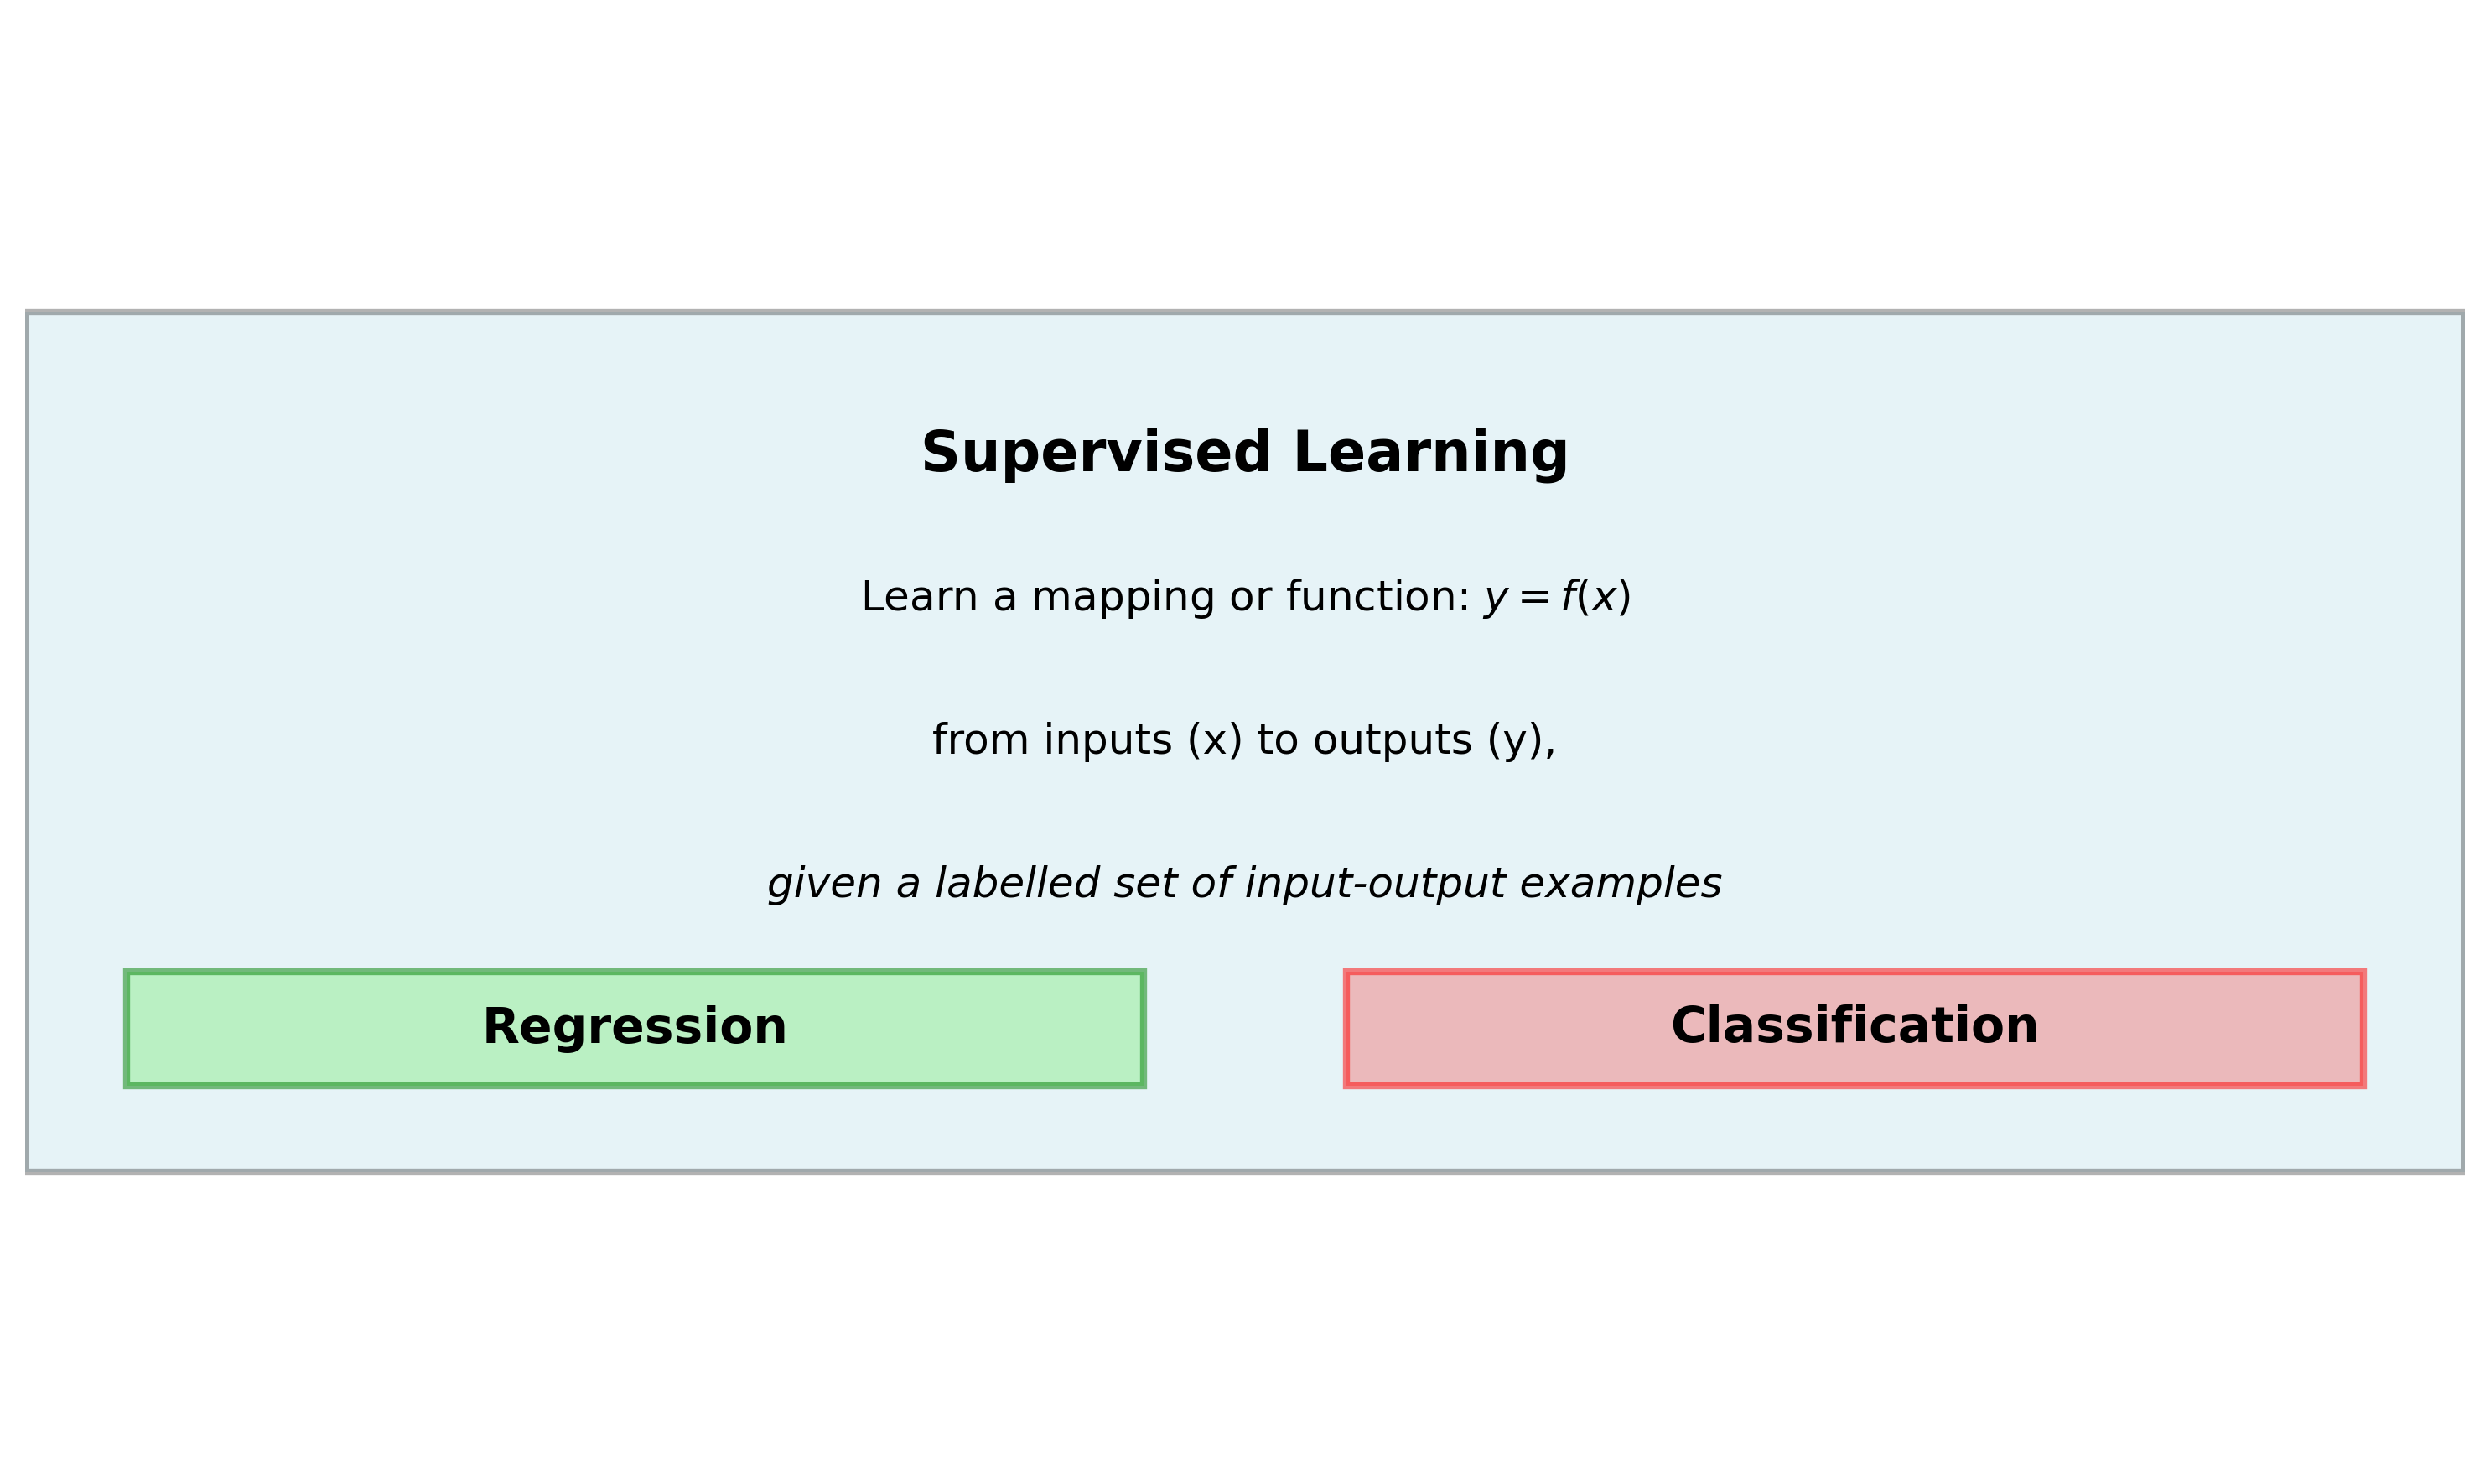
\includegraphics[width=0.75\textwidth]{../figures/supervised_learning_overview.png}

\vspace{0.3cm}
\begin{block}{Core Concept}
Given labeled training data $\{(x_1, y_1), (x_2, y_2), \ldots, (x_n, y_n)\}$, learn a function $f: \mathcal{X} \to \mathcal{Y}$ that maps inputs to outputs.
\end{block}

\begin{columns}[t]
\begin{column}{0.48\textwidth}
\begin{block}{Regression Tasks}
\begin{itemize}
\setlength{\itemsep}{1pt}
\item Continuous output values
\item Examples: price prediction, temperature
\item Algorithms: Linear/Polynomial regression, SVR
\end{itemize}
\end{block}
\end{column}

\begin{column}{0.48\textwidth}
\begin{block}{Classification Tasks}
\begin{itemize}
\setlength{\itemsep}{1pt}
\item Discrete class labels
\item Examples: spam detection, image recognition
\item Algorithms: Logistic regression, SVM
\end{itemize}
\end{block}
\end{column}
\end{columns}
\end{frame}

\begin{frame}{Comparison of Supervised Learning Methods}
\centering
\scriptsize
\begin{tabular}{|l|c|c|}
\hline
\textbf{Method} & \textbf{Model} & \textbf{Loss Function} \\
\hline
\textbf{Linear Regression} & $y = w^T x + b$ & $\sum_{i=1}^N (y_i - w^T x_i - b)^2$ \\
& & \textcolor{red}{Sum-of-squares loss} \\
\hline
\textbf{Logistic Regression} & $P(y=1|x) = \sigma(w^T x + b)$ & $-\sum_{i=1}^N y_i \log(\sigma(w^T x_i + b))$ \\
& $\sigma(z) = \frac{1}{1+e^{-z}}$ & $+ (1-y_i)\log(1-\sigma(w^T x_i + b))$ \\
& & \textcolor{red}{Cross-entropy loss} \\
\hline
\textbf{Support Vector Machine} & $y = \text{sign}(w^T x + b)$ & $\frac{1}{2}\|w\|^2 + C\sum_i \max(0, 1-y_i(w^T x_i + b))$ \\
& & \textcolor{red}{Hinge loss + L2 regularization} \\
\hline
\end{tabular}

\vspace{0.3cm}

\begin{alertblock}{Today's Focus}
We'll explore how \textbf{Support Vector Machines} use the \textcolor{blue}{\textbf{kernel trick}} to solve non-linear problems while maintaining computational efficiency.
\end{alertblock}
\end{frame}

\section{Introduction \& Motivation}

\begin{frame}{What are Kernel Methods?}
\begin{columns}[t]
\begin{column}{0.48\textwidth}
\begin{block}{Definition}
\textbf{Kernel methods} are a class of algorithms that use kernel functions to operate in high-dimensional feature spaces without explicitly computing the coordinates in that space.
\end{block}

\vspace{0.3cm}
\textbf{Key Idea:}
\begin{itemize}
\setlength{\itemsep}{1pt}
\item Transform data to higher dimensions where it becomes linearly separable
\item Use \textcolor{blue}{\textbf{kernel trick}} to avoid explicit transformation
\item Compute inner products efficiently in feature space
\end{itemize}

\vspace{0.3cm}
\begin{alertblock}{Why Kernel Methods?}
Many real-world problems are \textcolor{red}{\textbf{not linearly separable}} in their original feature space.
\end{alertblock}
\end{column}

\begin{column}{0.48\textwidth}
\textbf{Common Applications:}
\begin{itemize}
\setlength{\itemsep}{1pt}
\item \textcolor{green}{\textbf{Classification:}} Support Vector Machines
\item \textcolor{blue}{\textbf{Regression:}} Support Vector Regression
\item \textcolor{purple}{\textbf{Dimensionality Reduction:}} Kernel PCA
\item \textcolor{orange}{\textbf{Clustering:}} Kernel K-means
\end{itemize}

\vspace{0.3cm}
\textbf{Advantages:}
\begin{itemize}
\setlength{\itemsep}{1pt}
\item Handle non-linear relationships
\item Computational efficiency via kernel trick
\item Strong theoretical foundations
\item Flexible and powerful
\end{itemize}

\vspace{0.3cm}
\textbf{Examples:}
\begin{itemize}
\setlength{\itemsep}{1pt}
\item Image classification
\item Text analysis
\item Bioinformatics
\item Time series analysis
\end{itemize}
\end{column}
\end{columns}
\end{frame}

\begin{frame}{Linear vs Non-linear Separability}
\centering
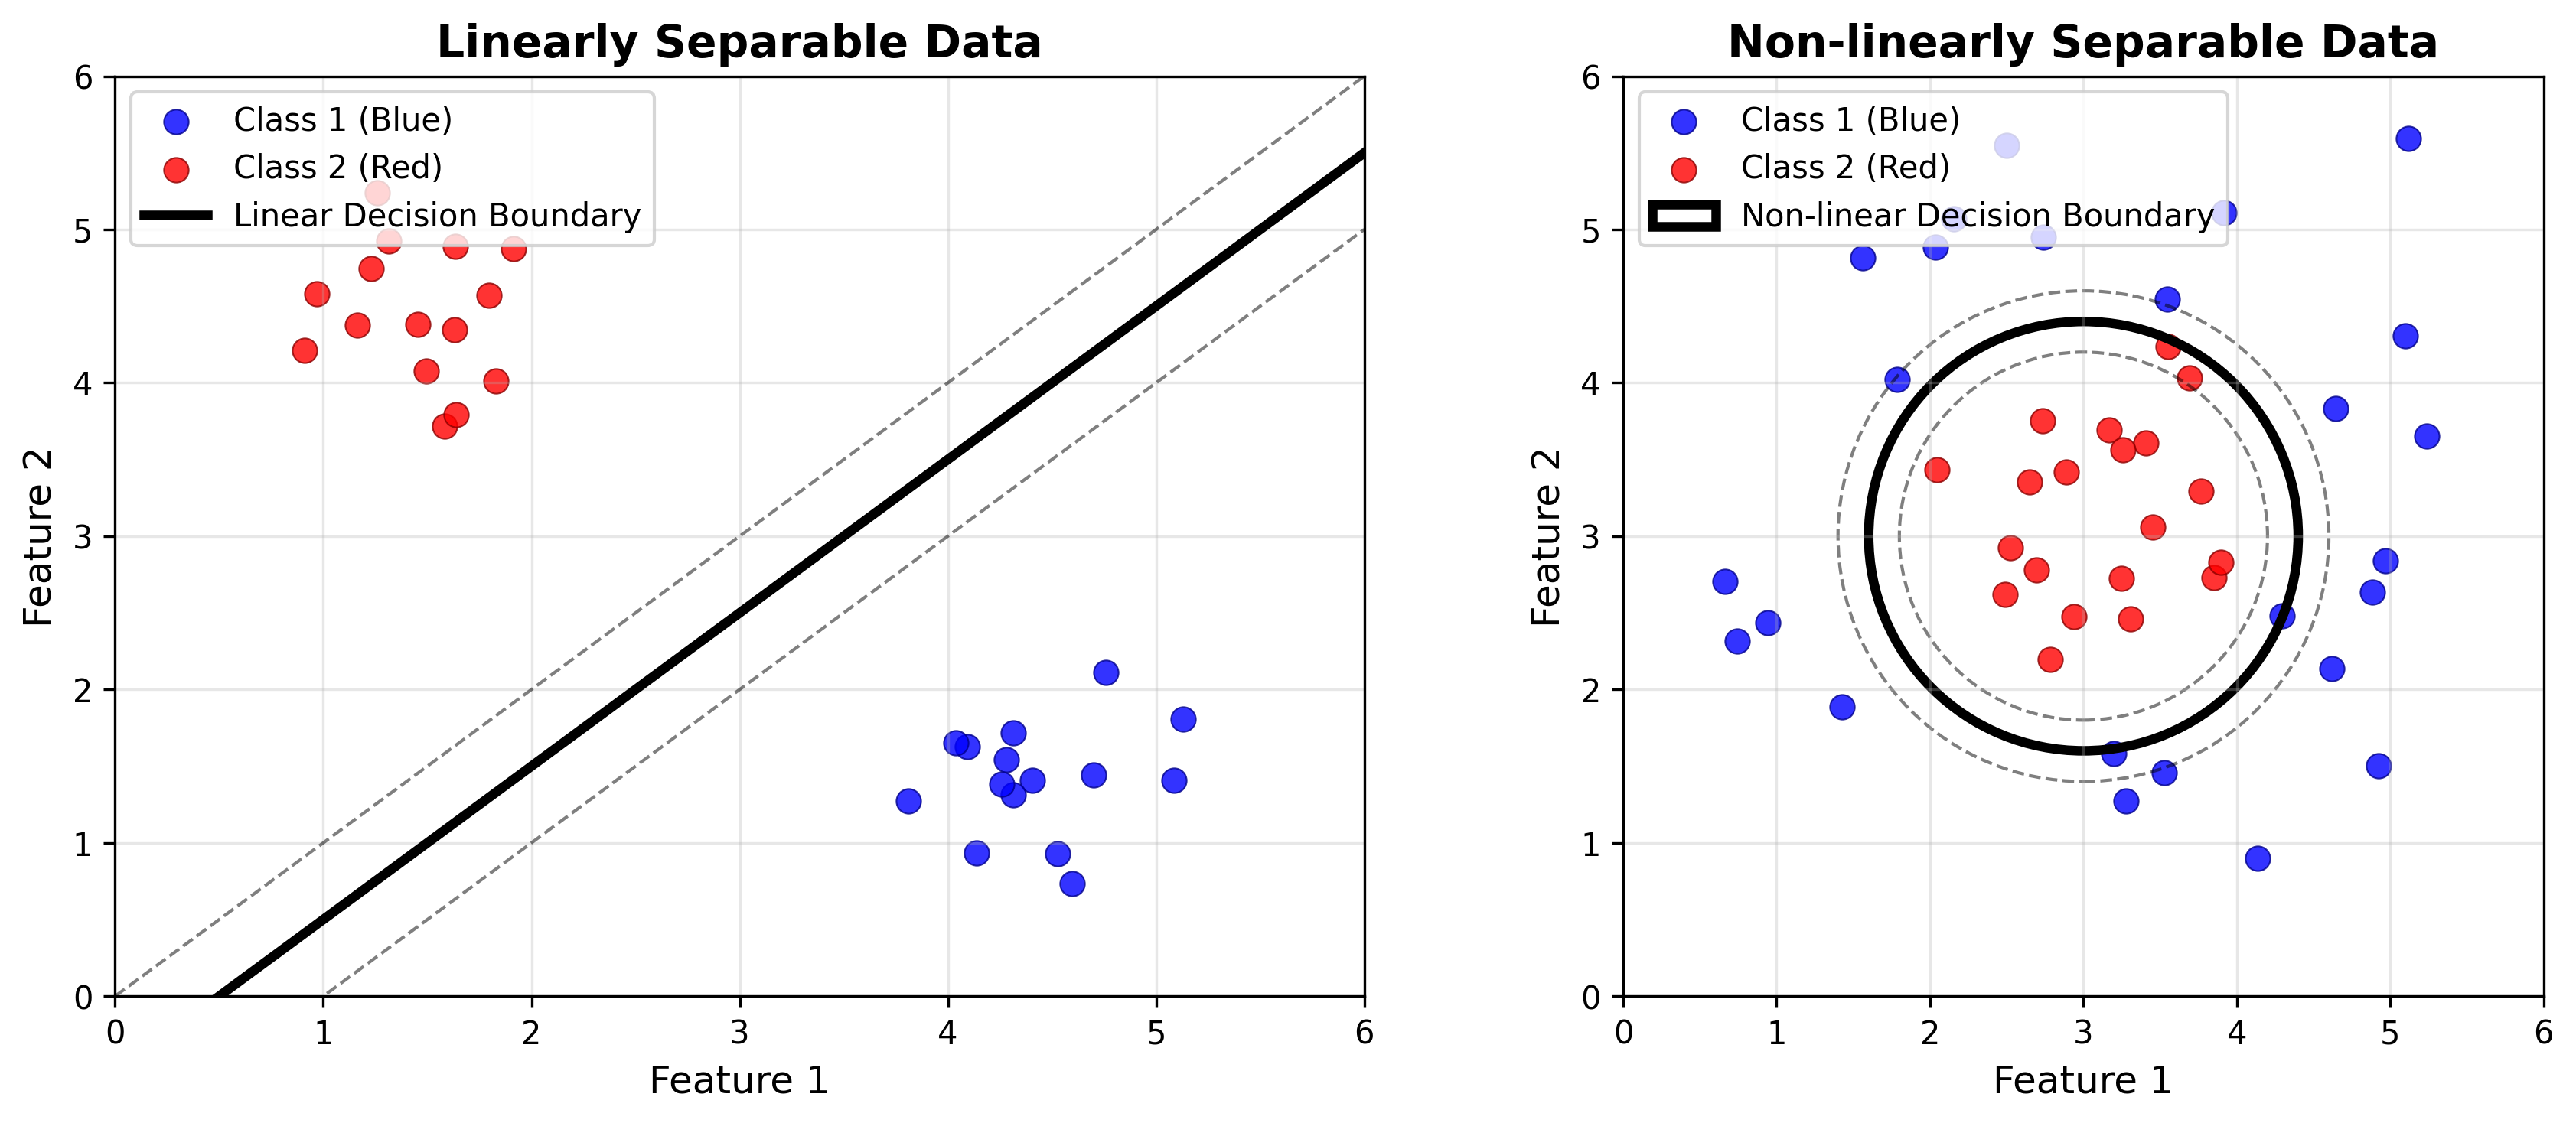
\includegraphics[width=0.8\textwidth]{../figures/linear_vs_nonlinear_data.png}

\vspace{0.2cm}
\begin{columns}[t]
\begin{column}{0.48\textwidth}
\begin{block}{Linearly Separable Data}
\textbf{Characteristics:}
\begin{itemize}
\setlength{\itemsep}{1pt}
\item Classes form distinct clusters
\item Linear boundary separates perfectly
\item Decision rule: $w^T x + b = 0$
\end{itemize}
\end{block}

\textbf{Advantages:}
\begin{itemize}
\setlength{\itemsep}{1pt}
\item Simple and interpretable
\item Fast training and prediction
\item Good generalization
\end{itemize}
\end{column}

\begin{column}{0.48\textwidth}
\begin{block}{Non-linearly Separable Data}
\textbf{Characteristics:}
\begin{itemize}
\setlength{\itemsep}{1pt}
\item Complex data patterns (e.g., concentric circles)
\item No linear boundary can separate
\item Requires non-linear decision boundary
\end{itemize}
\end{block}

\textbf{Solution: Kernel Methods}
\begin{itemize}
\setlength{\itemsep}{1pt}
\item Transform to higher dimensions
\item Apply linear methods in new space
\item Kernel trick for efficiency
\end{itemize}
\end{column}
\end{columns}
\end{frame}

\section{Historical Context: From Perceptron to SVM}

\begin{frame}{Rosenblatt's Perceptron (1957)}
\begin{columns}[t]
\begin{column}{0.48\textwidth}
\begin{block}{The Perceptron Algorithm}
\textbf{Frank Rosenblatt} introduced the first learning algorithm for binary classification in 1957.
\end{block}

\vspace{0.3cm}
\textbf{Perceptron Model:}
\begin{align}
f(x) &= \text{sign}(w^T x + b) \\
\text{Output} &= \begin{cases}
+1 & \text{if } w^T x + b \geq 0 \\
-1 & \text{if } w^T x + b < 0
\end{cases}
\end{align}

\vspace{0.3cm}
\textbf{Learning Rule:}
\begin{align}
w^{(t+1)} &= w^{(t)} + \eta \cdot y_i \cdot x_i \\
b^{(t+1)} &= b^{(t)} + \eta \cdot y_i
\end{align}
\textit{Update only when misclassified}

\vspace{0.3cm}
\begin{alertblock}{Perceptron Convergence Theorem}
If data is linearly separable, the perceptron algorithm will converge to a solution in finite steps.
\end{alertblock}
\end{column}

\begin{column}{0.48\textwidth}
\textbf{Historical Impact:}
\vspace{0.2cm}

\begin{itemize}
\setlength{\itemsep}{2pt}
\item \textbf{1957:} Perceptron introduced
\item \textbf{1969:} Limitations exposed (XOR problem)
\item \textbf{1980s-1990s:} SVM development
\item \textbf{Key insight:} Maximum margin principle
\end{itemize}

\vspace{0.3cm}
\textbf{Motivation for SVMs:}
\begin{itemize}
\setlength{\itemsep}{1pt}
\item Address perceptron limitations
\item Better generalization bounds
\item Handle non-linearly separable data
\end{itemize}
\end{column}
\end{columns}
\end{frame}

\begin{frame}{Perceptron vs SVM: A Visual Comparison}
\centering
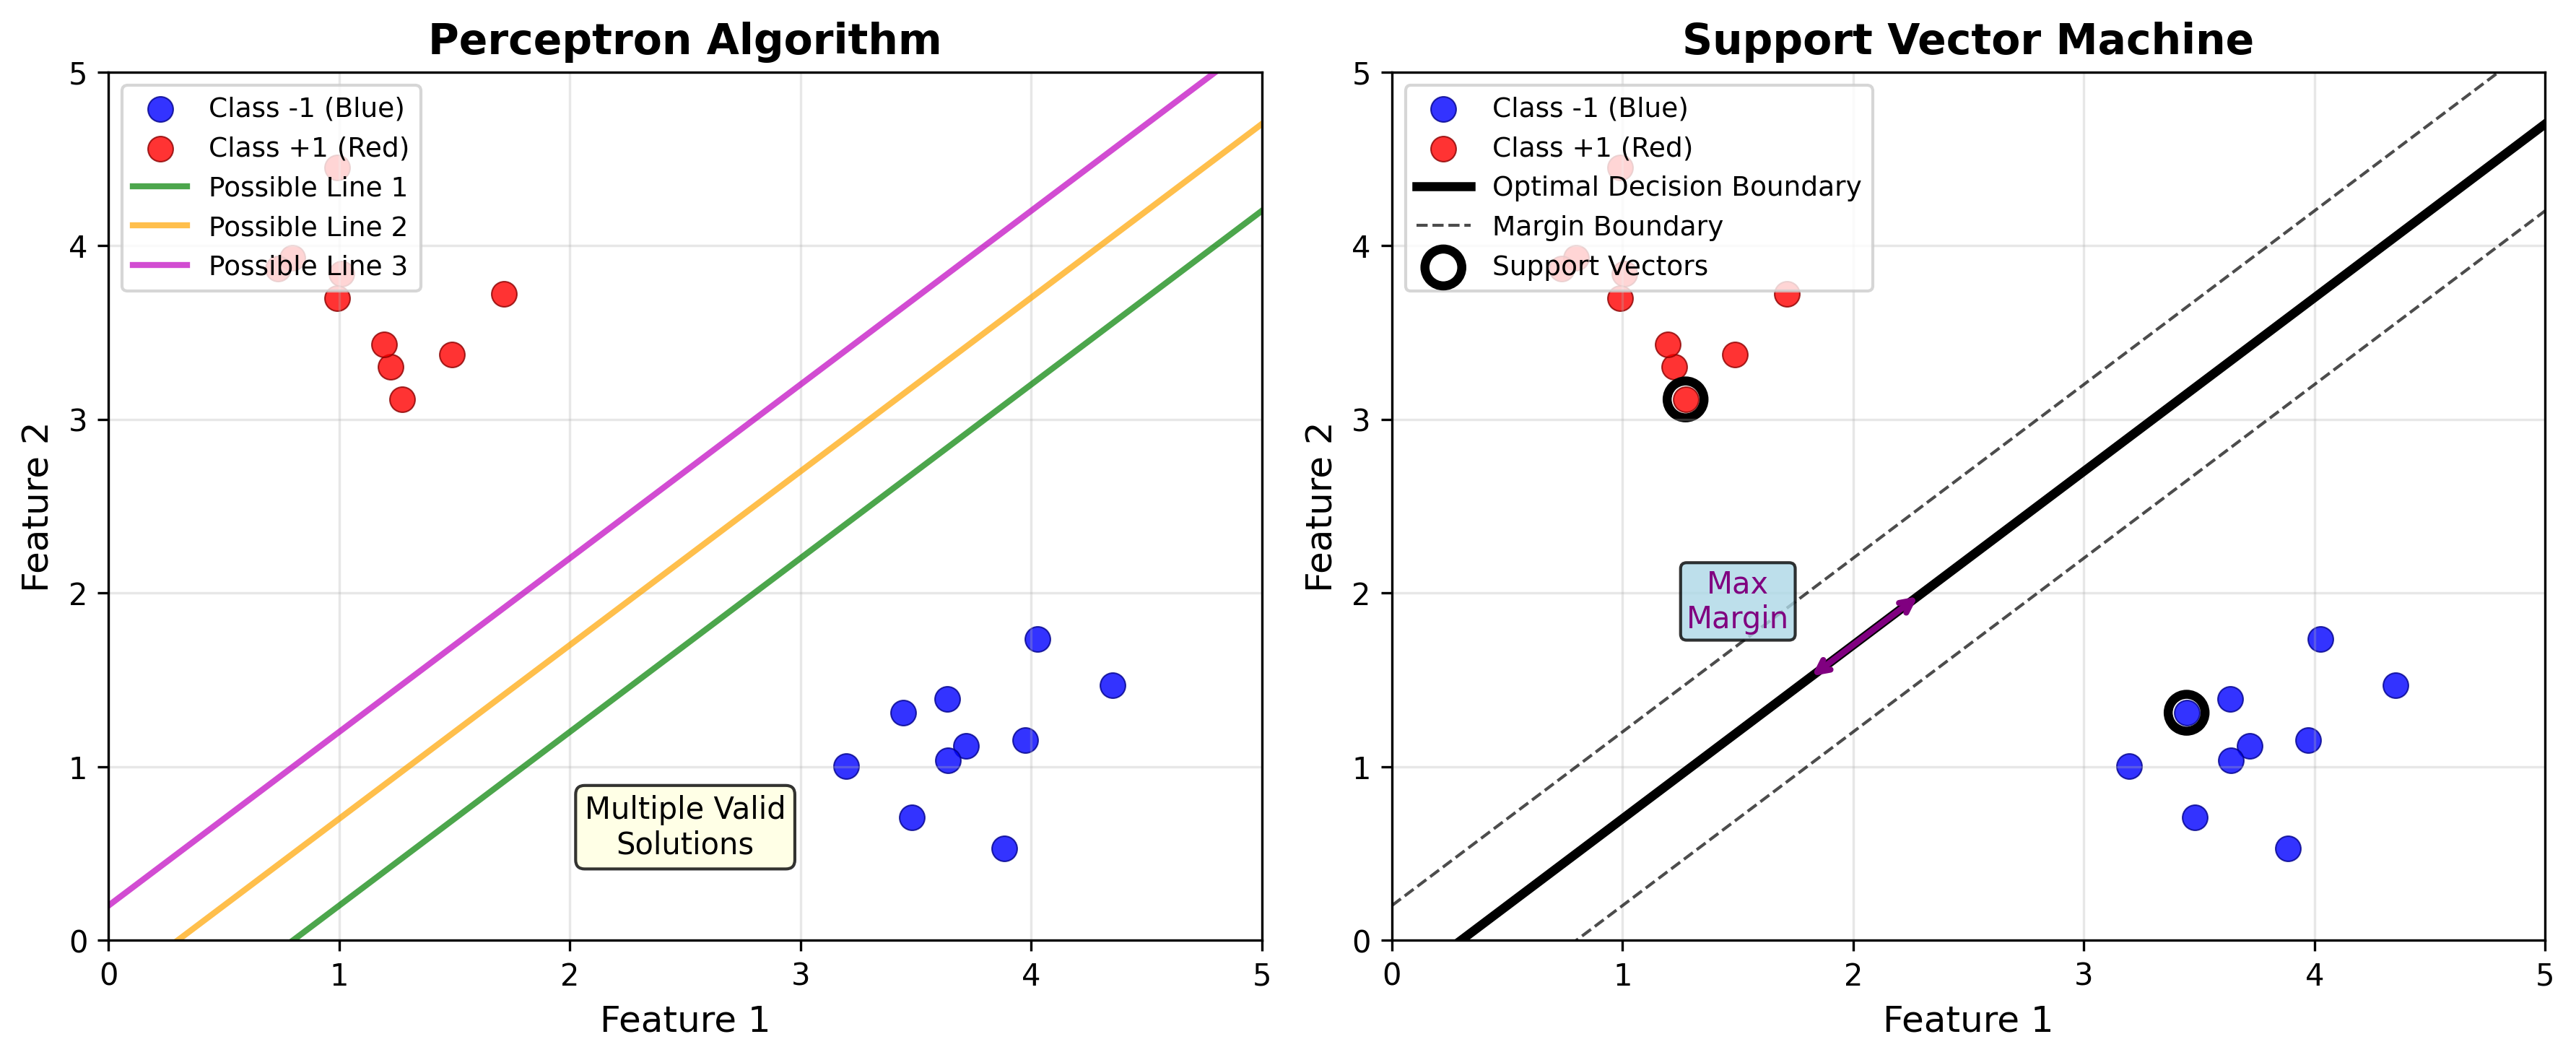
\includegraphics[width=0.85\textwidth]{../figures/perceptron_vs_svm.png}

\vspace{0.3cm}
\begin{columns}[t]
\begin{column}{0.48\textwidth}
\begin{block}{Perceptron Approach}
\begin{itemize}
\setlength{\itemsep}{1pt}
\item \textbf{Goal:} Find any separating hyperplane
\item \textbf{Method:} Iterative weight updates
\item \textbf{Result:} Multiple valid solutions
\item \textbf{Issue:} No optimality criterion
\end{itemize}
\end{block}
\end{column}

\begin{column}{0.48\textwidth}
\begin{block}{SVM Approach}
\begin{itemize}
\setlength{\itemsep}{1pt}
\item \textbf{Goal:} Find optimal separating hyperplane
\item \textbf{Method:} Maximize margin width
\item \textbf{Result:} Unique optimal solution
\item \textbf{Benefit:} Better generalization
\end{itemize}
\end{block}
\end{column}
\end{columns}

\begin{alertblock}{Key Insight}
SVMs choose the hyperplane that maximizes the distance to the nearest data points (\textbf{support vectors}), leading to better generalization performance.
\end{alertblock}
\end{frame}

\begin{frame}{From Linear to Non-linear: Evolution of Ideas}
\begin{columns}[t]
\begin{column}{0.48\textwidth}
\textbf{Timeline of Development:}
\vspace{0.2cm}

\begin{itemize}
\setlength{\itemsep}{2pt}
\item \textbf{1957:} Rosenblatt's Perceptron
\item \textbf{1969:} Minsky \& Papert limitations
\item \textbf{1979:} Least squares SVM ideas
\item \textbf{1992:} Boser, Guyon, Vapnik kernel trick
\item \textbf{1995:} Cortes \& Vapnik soft margin
\item \textbf{1996:} Schölkopf kernel methods
\end{itemize}

\vspace{0.3cm}
\begin{block}{Minsky \& Papert (1969)}
Showed that perceptrons cannot solve non-linearly separable problems like XOR, leading to the "AI winter."
\end{block}

\vspace{0.3cm}
\begin{alertblock}{The Kernel Revolution}
The kernel trick (1992) revived interest by enabling non-linear classification while maintaining computational efficiency.
\end{alertblock}
\end{column}

\begin{column}{0.48\textwidth}
\textbf{The XOR Problem:}
\vspace{0.2cm}

\centering
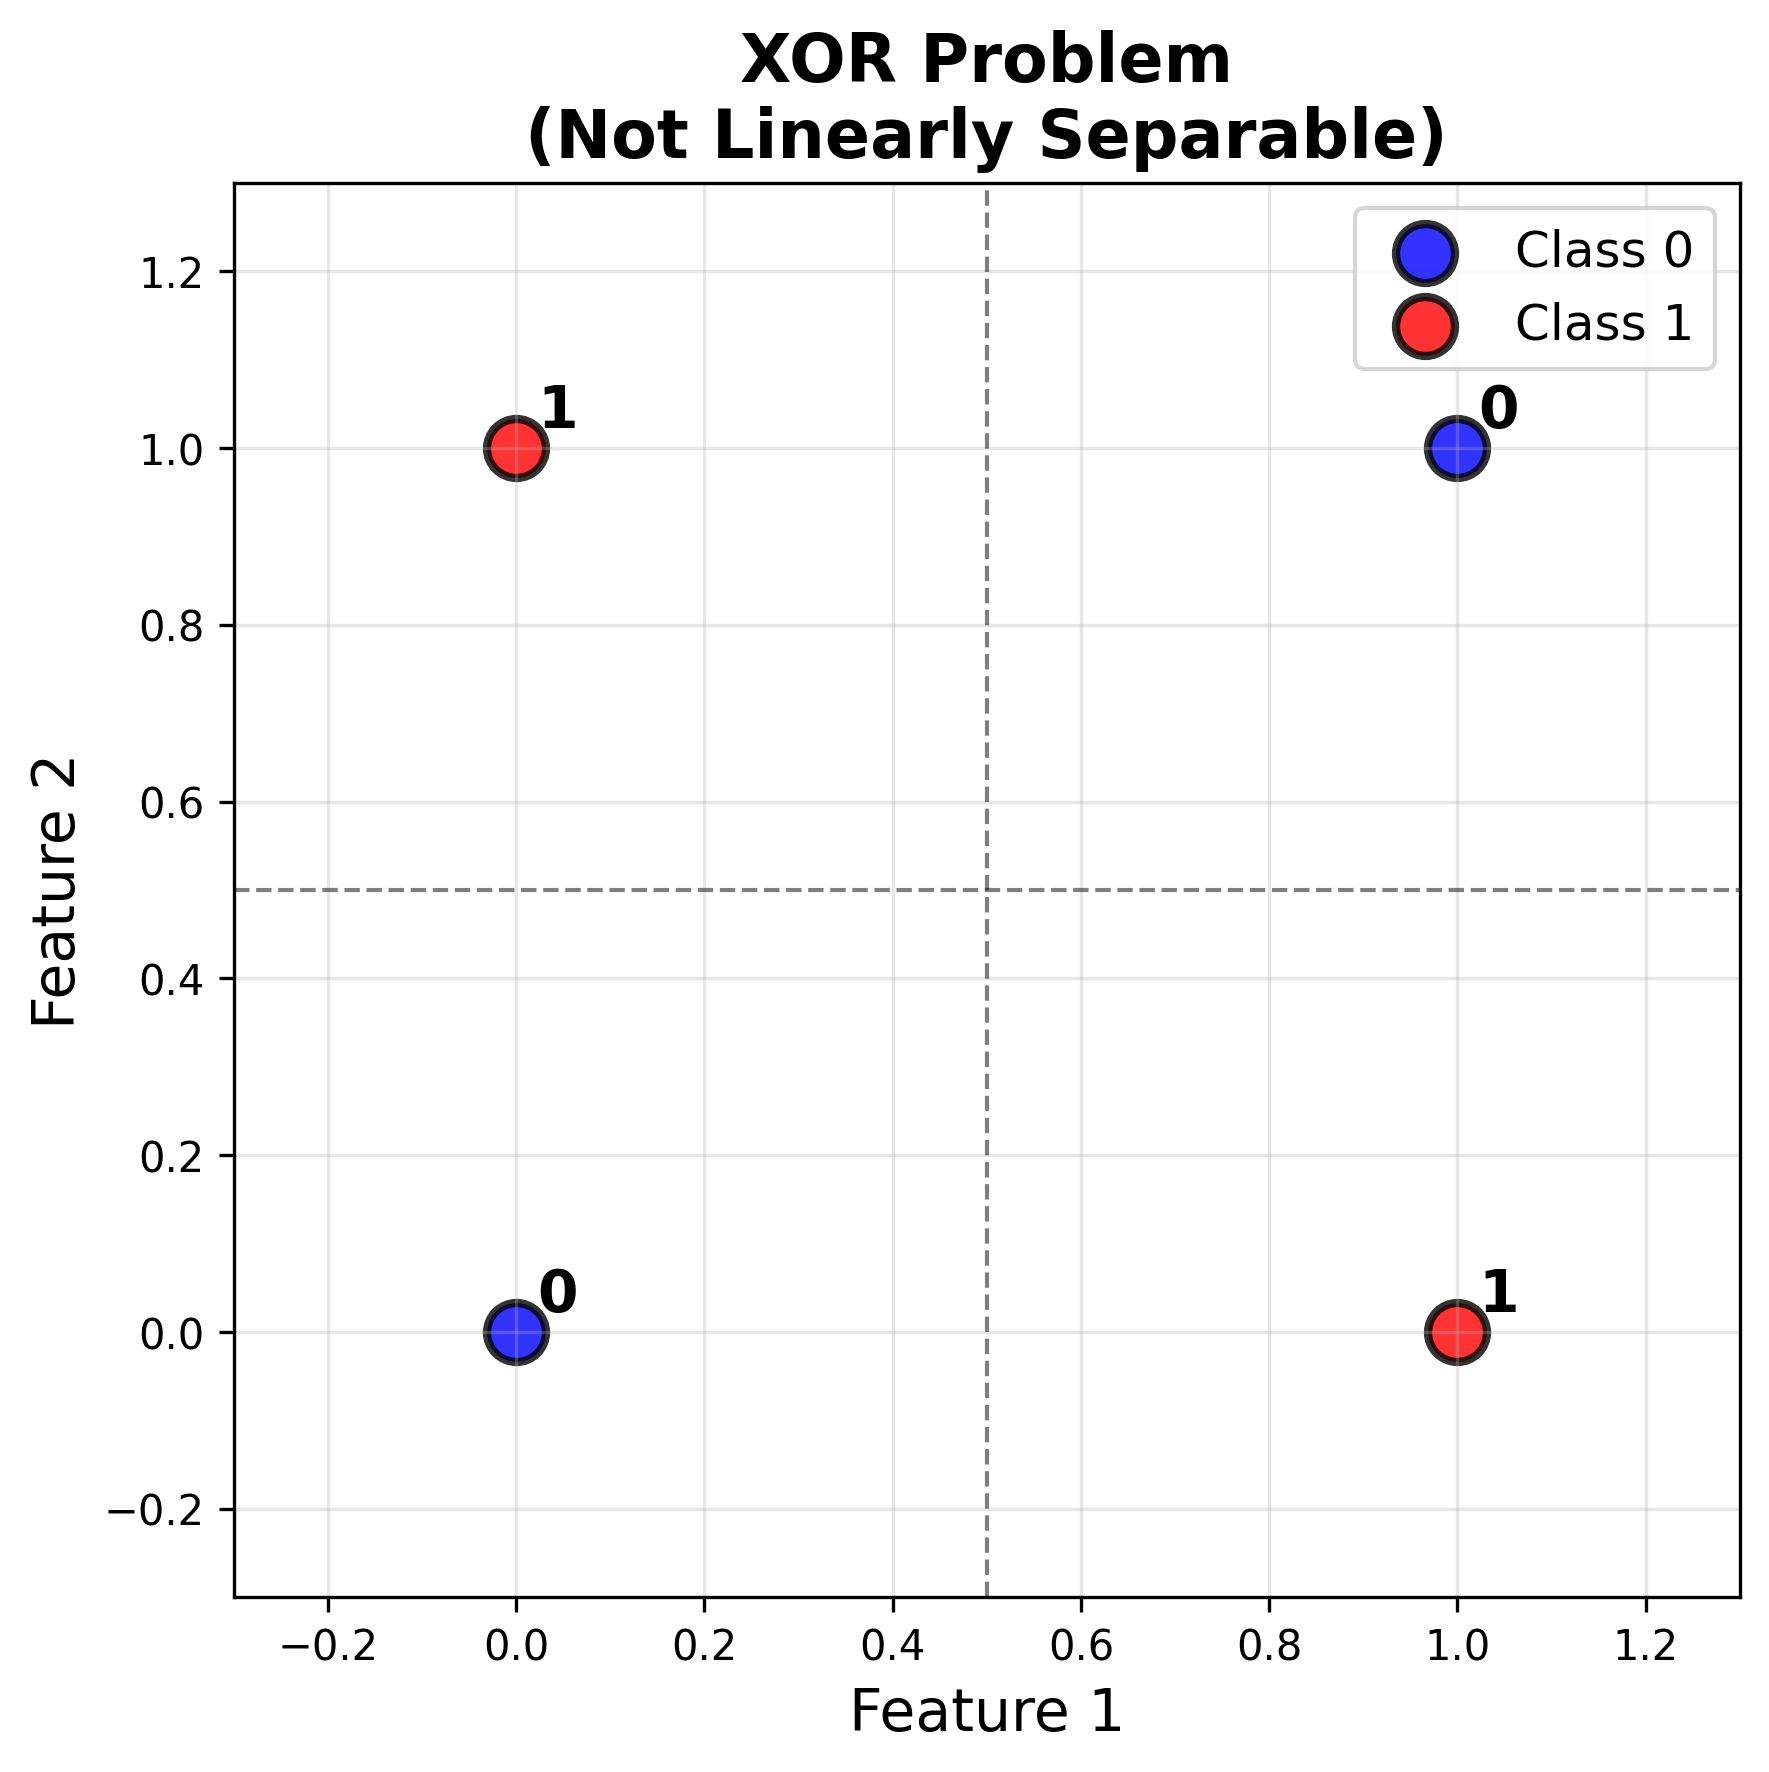
\includegraphics[width=0.8\textwidth]{../figures/xor_problem.png}

\vspace{0.2cm}
\begin{block}{Problem Statement}
\begin{itemize}
\setlength{\itemsep}{1pt}
\item Input: $(0,0) \to 0$, $(0,1) \to 1$
\item Input: $(1,0) \to 1$, $(1,1) \to 0$
\item \textcolor{red}{No linear separator exists}
\end{itemize}
\end{block}

\vspace{0.2cm}
\textbf{Kernel Solution:}
Transform to 3D space:
$$\phi(x_1, x_2) = (x_1, x_2, x_1 x_2)$$

\textcolor{green}{\textbf{Result:}} Linearly separable in 3D!
\end{column}
\end{columns}
\end{frame}

\section{Support Vector Machines}

\begin{frame}{Support Vector Machines: Overview}
\begin{columns}[t]
\begin{column}{0.48\textwidth}
\begin{block}{Core Concept}
\textbf{SVM} finds the optimal hyperplane that separates classes with the \textcolor{blue}{\textbf{maximum margin}}.
\end{block}

\vspace{0.3cm}
\textbf{Key Components:}
\begin{itemize}
\setlength{\itemsep}{1pt}
\item \textbf{Decision boundary:} Hyperplane separating classes
\item \textbf{Margin:} Distance between boundary and closest points
\item \textbf{Support vectors:} Points defining the margin
\end{itemize}

\vspace{0.3cm}
\textbf{Mathematical Formulation:}
\begin{align}
\text{Hyperplane: } &\quad w^T x + b = 0 \\
\text{Margin: } &\quad \frac{2}{\|w\|}
\end{align}

\begin{alertblock}{Goal}
\textcolor{red}{\textbf{Maximize margin}} while correctly classifying all training points.
\end{alertblock}
\end{column}

\begin{column}{0.48\textwidth}
\begin{center}
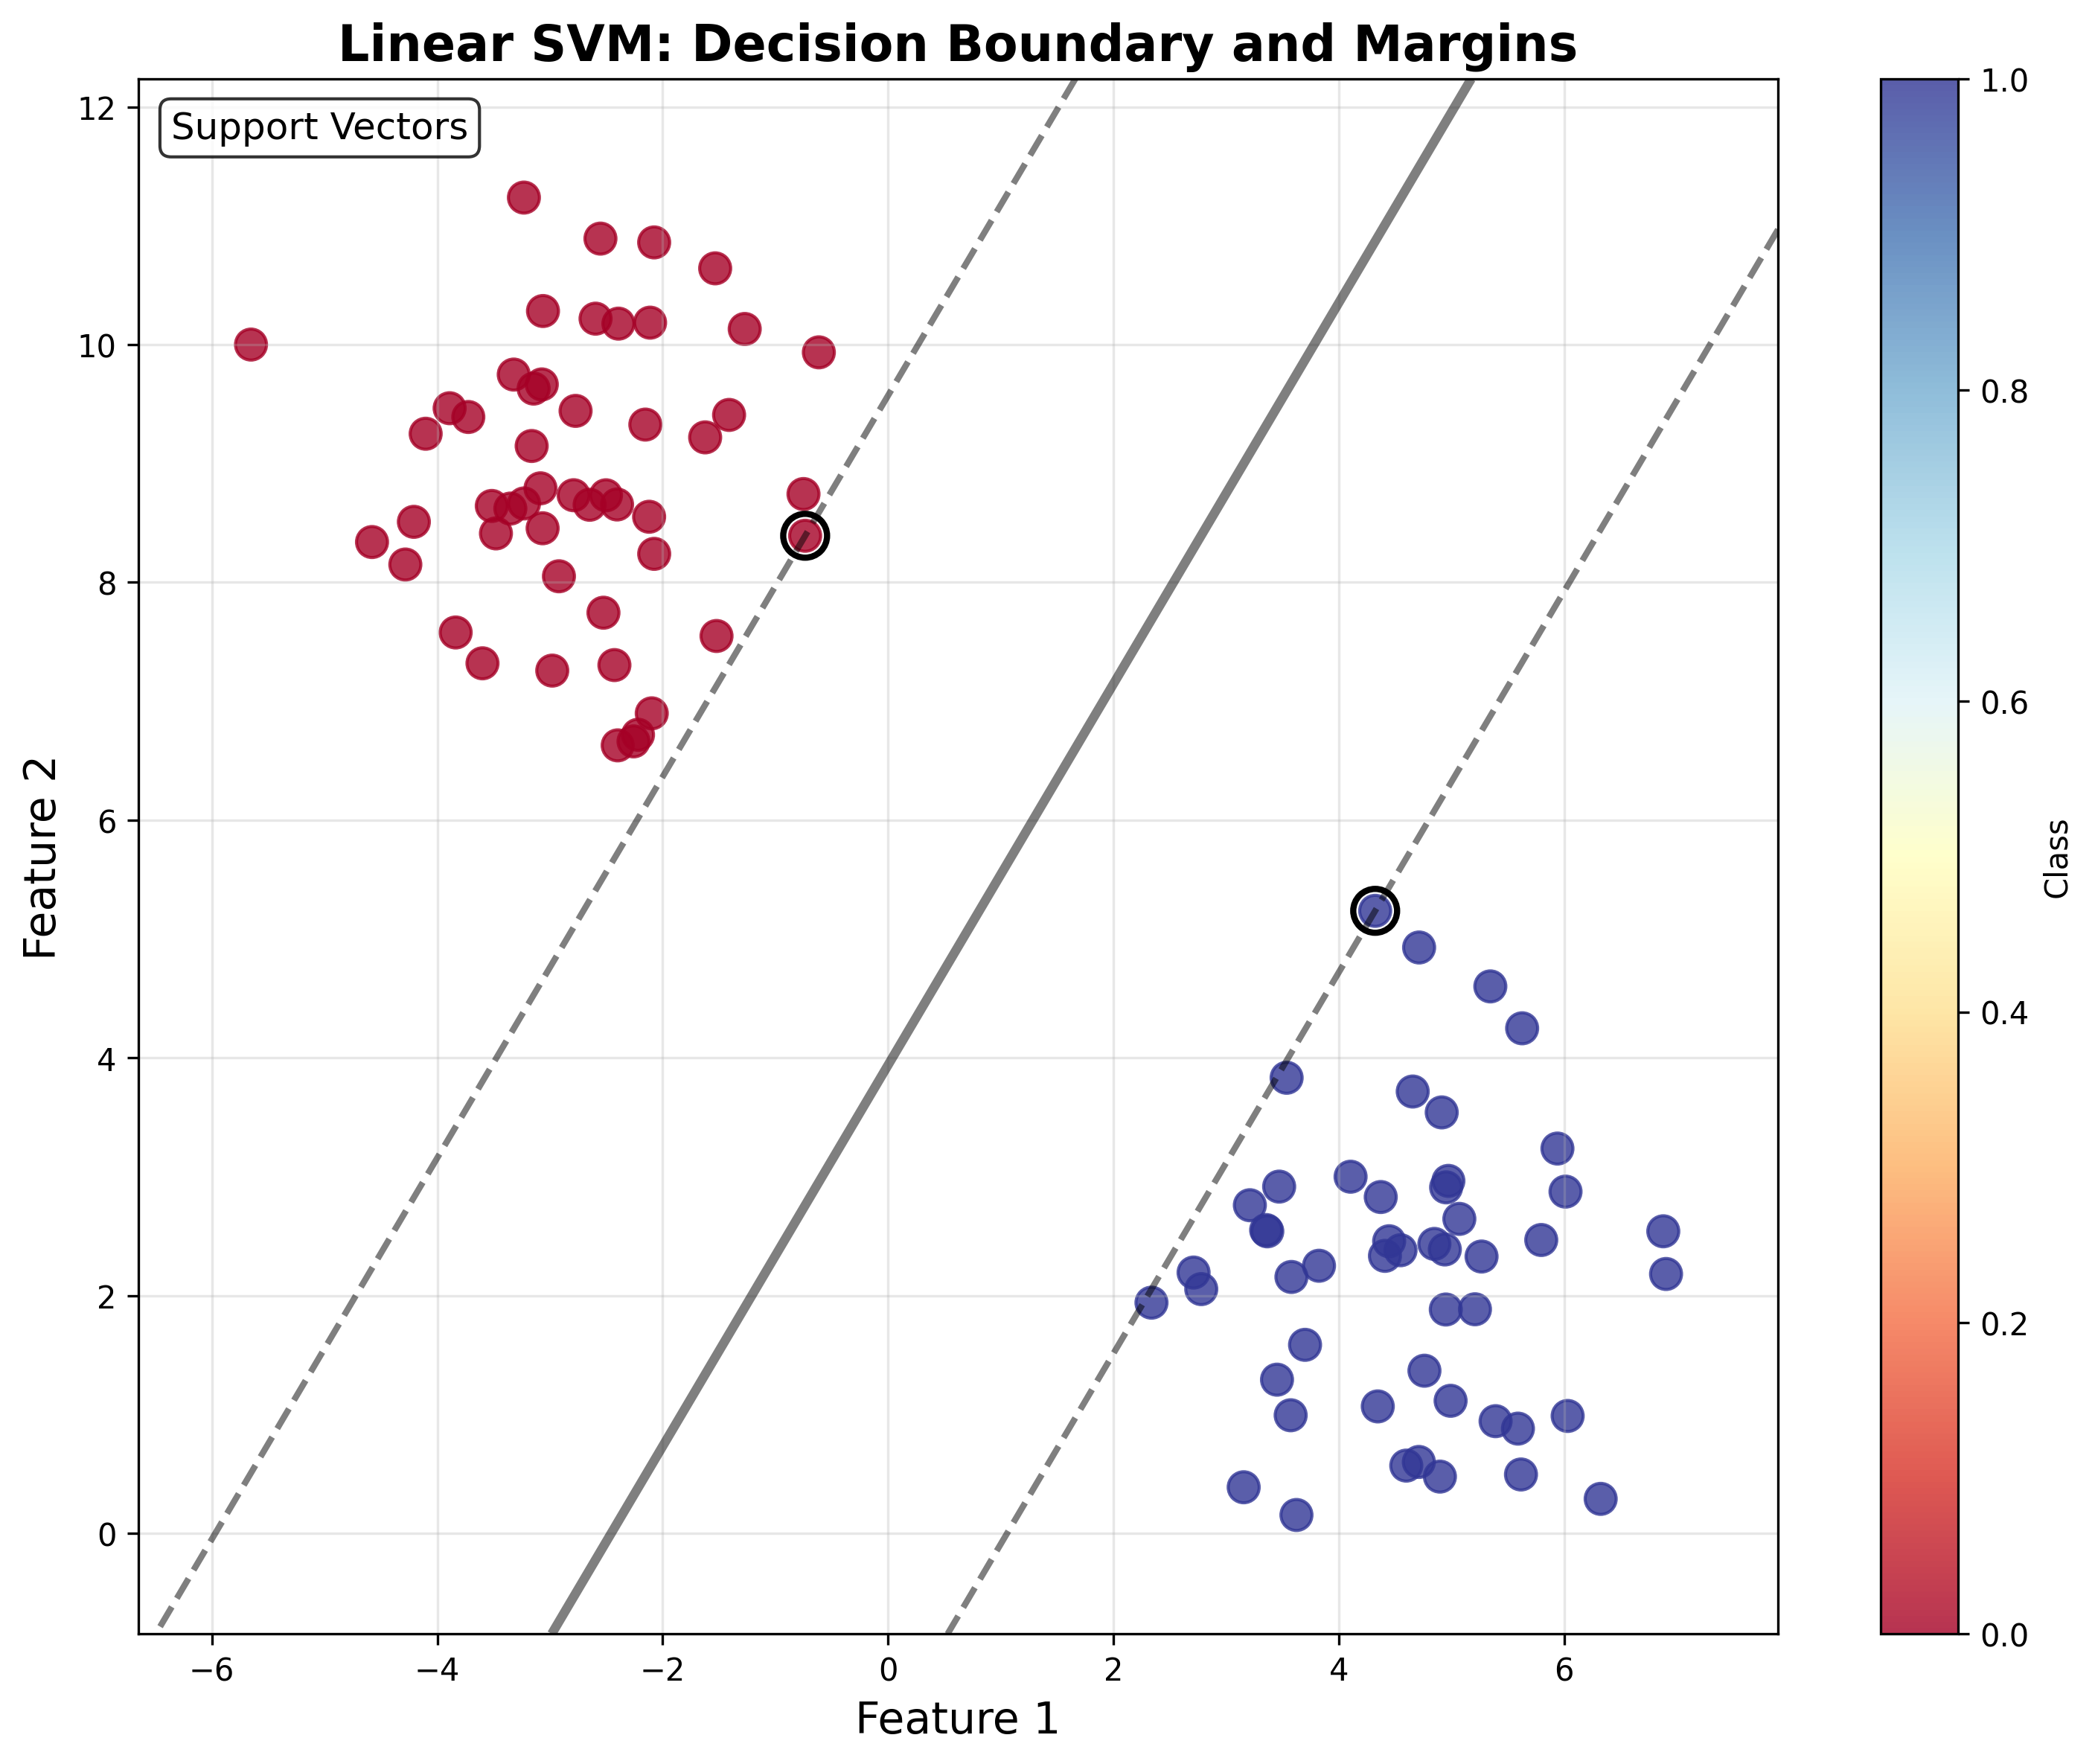
\includegraphics[width=\textwidth]{../figures/linear_svm_margins.png}
\end{center}

\vspace{0.2cm}
\textbf{Why Maximum Margin?}
\begin{itemize}
\setlength{\itemsep}{1pt}
\item \textcolor{green}{\textbf{Generalization:}} Better performance on unseen data
\item \textcolor{blue}{\textbf{Robustness:}} Less sensitive to noise
\item \textcolor{purple}{\textbf{Uniqueness:}} Single optimal solution
\end{itemize}
\end{column}
\end{columns}
\end{frame}

\section{Large-Margin Classifiers}

\begin{frame}{Geometric Interpretation of Margin}
\begin{columns}[t]
\begin{column}{0.48\textwidth}
\textbf{Margin Definition:}
\vspace{0.2cm}

For a hyperplane $w^T x + b = 0$:
\begin{align}
\text{Distance from point } x_i \text{ to hyperplane:} \\
d_i = \frac{|w^T x_i + b|}{\|w\|}
\end{align}

\vspace{0.3cm}
\textbf{Margin Width:}
\begin{align}
\text{Margin} = \min_{i} d_i = \frac{1}{\|w\|}
\end{align}

\vspace{0.3cm}
\begin{block}{Canonical Form}
Scale $w$ and $b$ so that for the closest points:
$$w^T x_i + b = \pm 1$$
Then margin becomes $\frac{2}{\|w\|}$.
\end{block}
\end{column}

\begin{column}{0.48\textwidth}
\textbf{Visual Interpretation:}
\vspace{0.2cm}

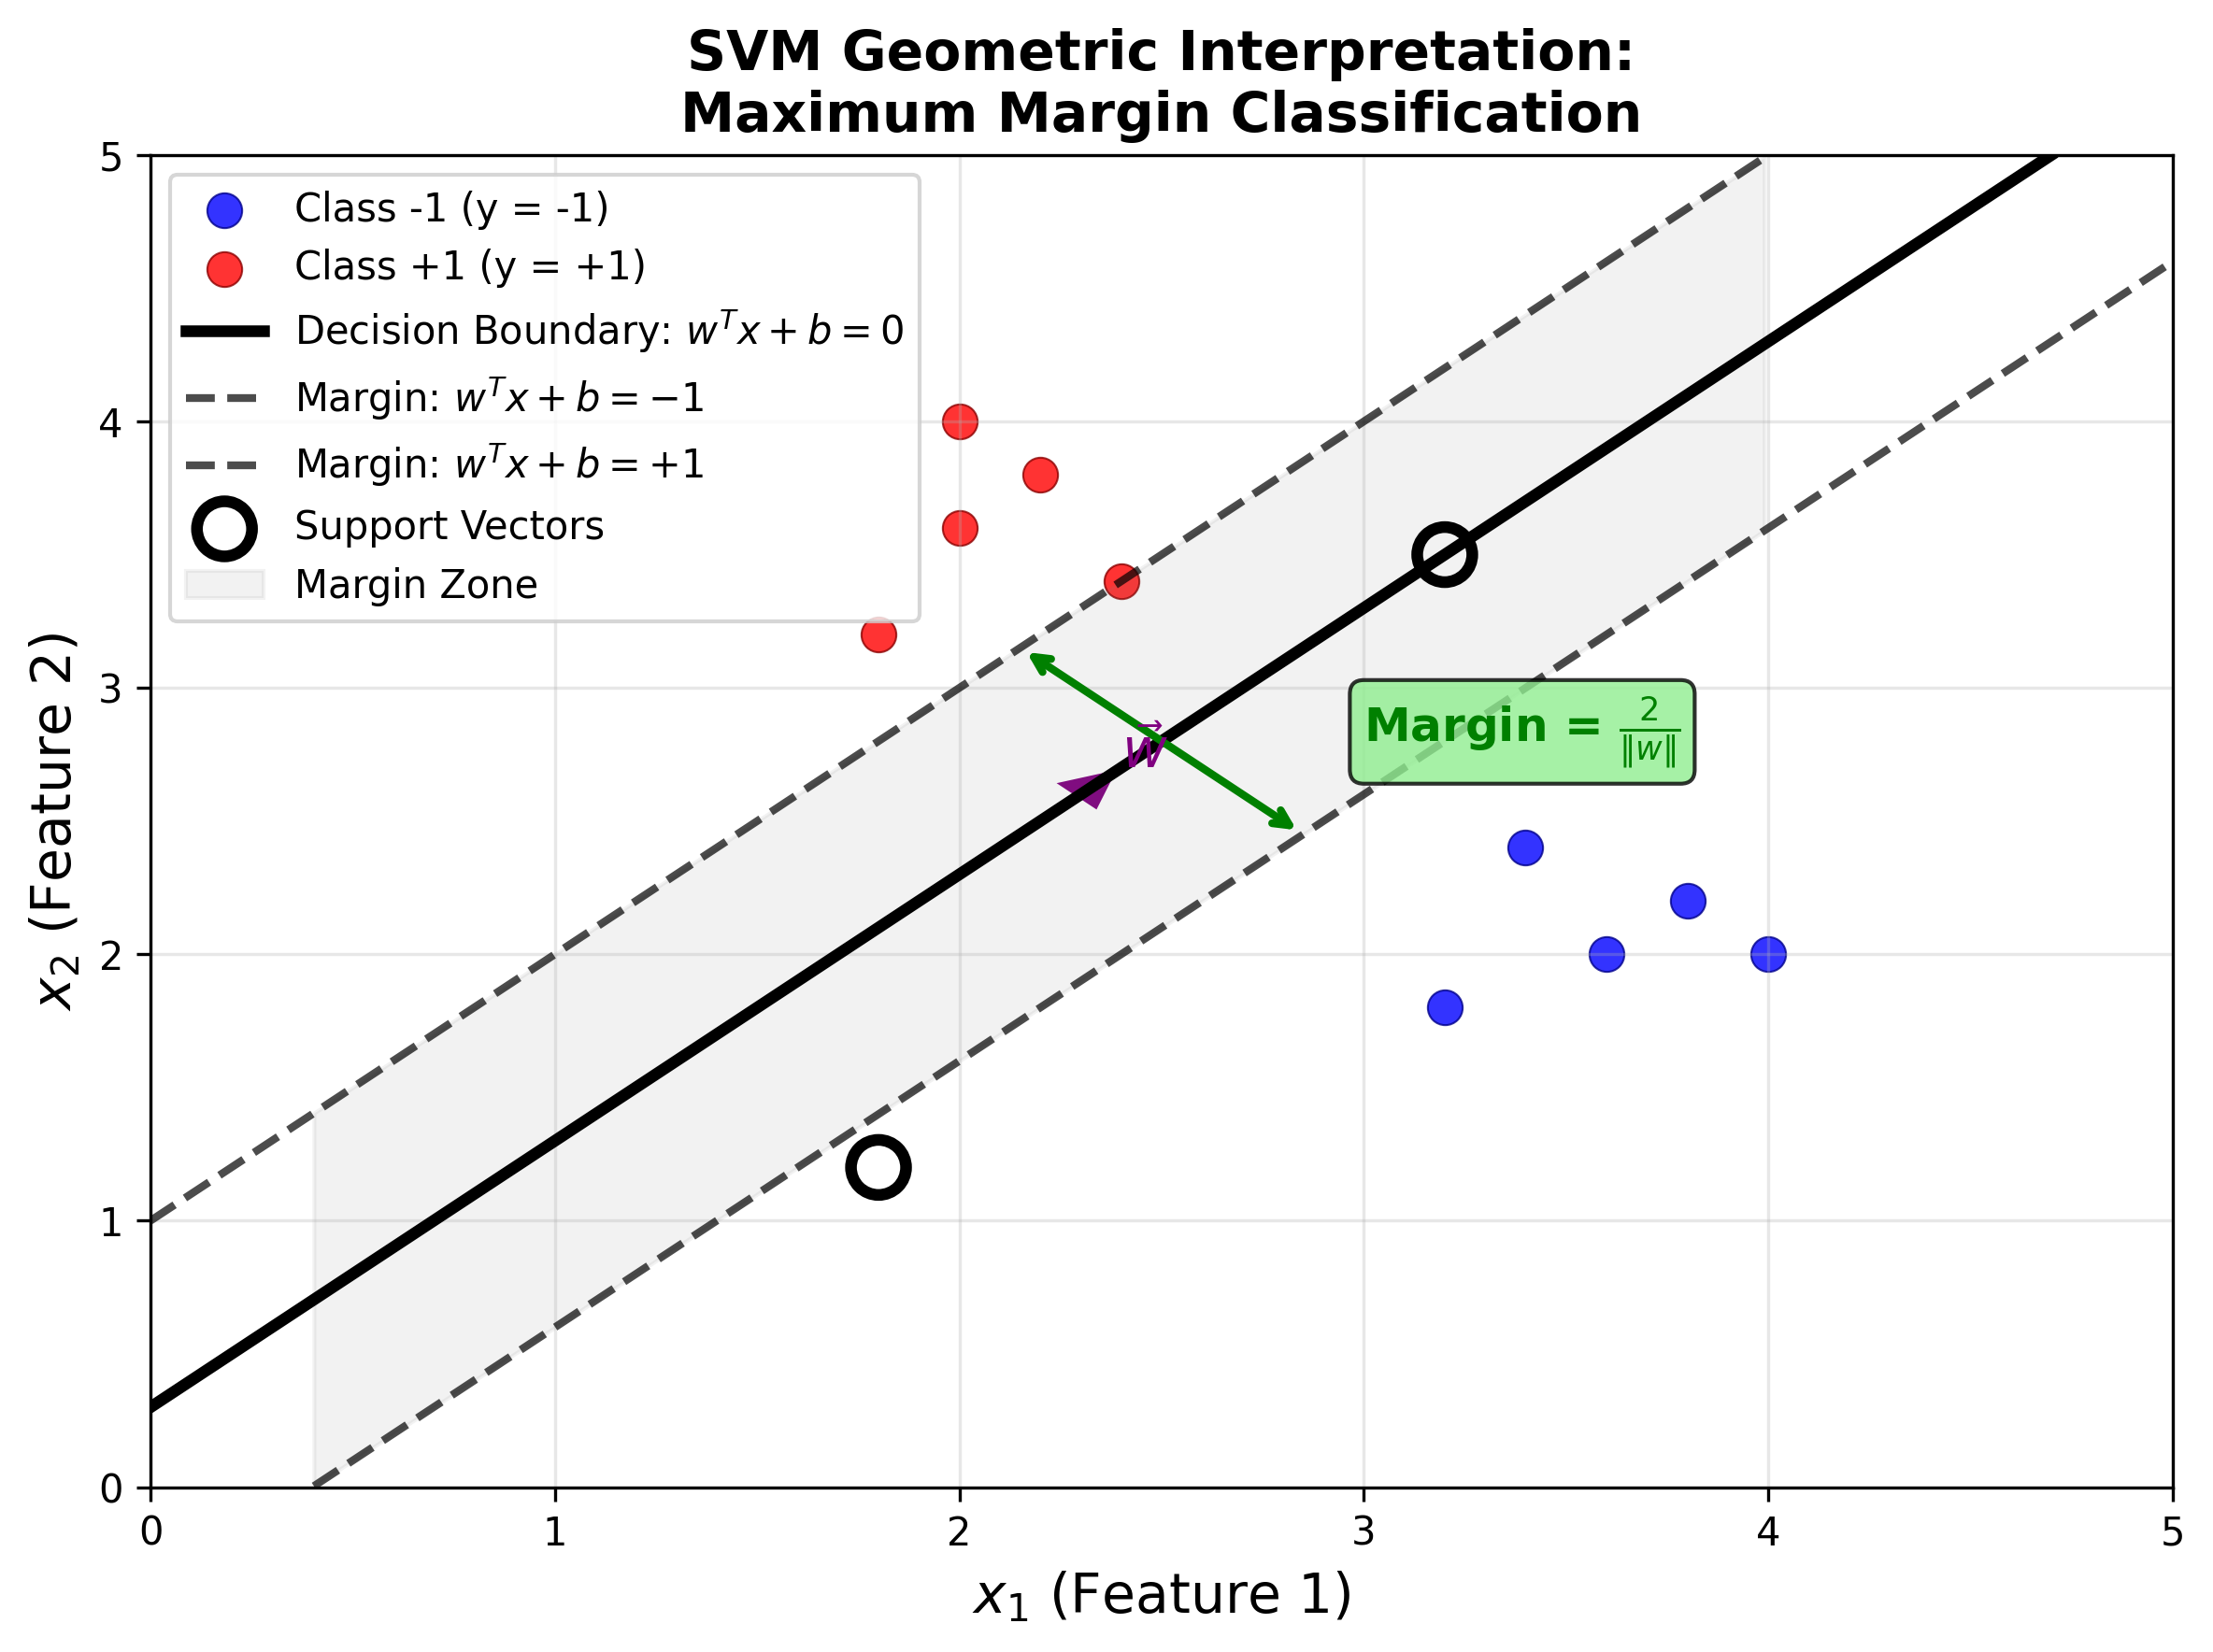
\includegraphics[width=0.95\textwidth]{../figures/svm_geometry.png}

\vspace{0.2cm}
\begin{block}{Key Elements}
\begin{itemize}
\setlength{\itemsep}{1pt}
\item \textcolor{blue}{\textbf{Decision boundary:}} $w^T x + b = 0$
\item \textcolor{red}{\textbf{Margin boundaries:}} $w^T x + b = \pm 1$
\item \textcolor{black}{\textbf{Support vectors:}} Closest points
\item \textcolor{green}{\textbf{Margin width:}} $\frac{2}{\|w\|}$
\end{itemize}
\end{block}
\end{column}
\end{columns}
\end{frame}

\section{Quadratic Optimization Problem}

\begin{frame}{SVM Optimization: Primal Problem}
\begin{columns}[t]
\begin{column}{0.48\textwidth}
\textbf{Hard Margin SVM:}
\vspace{0.2cm}

\begin{block}{Primal Problem}
\begin{align}
\min_{w,b} \quad &\frac{1}{2}\|w\|^2 \\
\text{subject to} \quad &y_i(w^T x_i + b) \geq 1, \quad i = 1,\ldots,n
\end{align}
\end{block}

\vspace{0.3cm}
\textbf{Interpretation:}
\begin{itemize}
\setlength{\itemsep}{1pt}
\item \textcolor{blue}{\textbf{Objective:}} Minimize $\|w\|^2$ $\Rightarrow$ Maximize margin $\frac{2}{\|w\|}$
\item \textcolor{red}{\textbf{Constraints:}} All points correctly classified with margin $\geq 1$
\end{itemize}

\vspace{0.3cm}
\textbf{Problem Type:}
\begin{itemize}
\setlength{\itemsep}{1pt}
\item Quadratic objective function
\item Linear constraints
\item Convex optimization problem
\item Unique global optimum
\end{itemize}
\end{column}

\begin{column}{0.48\textwidth}
\textbf{Soft Margin SVM:}
\vspace{0.2cm}

\begin{block}{Primal Problem with Slack Variables}
\begin{align}
\min_{w,b,\xi} \quad &\frac{1}{2}\|w\|^2 + C\sum_{i=1}^{n}\xi_i \\
\text{subject to} \quad &y_i(w^T x_i + b) \geq 1 - \xi_i \\
&\xi_i \geq 0, \quad i = 1,\ldots,n
\end{align}
\end{block}

\vspace{0.3cm}
\textbf{Slack Variables $\xi_i$:}
\begin{itemize}
\setlength{\itemsep}{1pt}
\item $\xi_i = 0$: Point correctly classified with margin $\geq 1$
\item $0 < \xi_i < 1$: Point correctly classified but within margin
\item $\xi_i \geq 1$: Point misclassified
\end{itemize}

\vspace{0.3cm}
\textbf{Regularization Parameter $C$:}
\begin{itemize}
\setlength{\itemsep}{1pt}
\item Large $C$: Penalty for violations (hard margin)
\item Small $C$: Allow more violations (soft margin)
\item Controls bias-variance tradeoff
\end{itemize}
\end{column}
\end{columns}
\end{frame}

\begin{frame}{SVM Optimization: Dual Problem}
\begin{columns}[t]
\begin{column}{0.48\textwidth}
\textbf{Lagrangian Formulation:}
\vspace{0.2cm}

\begin{block}{Lagrangian}
\begin{align}
L = &\frac{1}{2}\|w\|^2 + C\sum_{i=1}^{n}\xi_i \\
&- \sum_{i=1}^{n}\alpha_i[y_i(w^T x_i + b) - 1 + \xi_i] \\
&- \sum_{i=1}^{n}\mu_i\xi_i
\end{align}
\end{block}

\vspace{0.3cm}
\textbf{KKT Conditions:}
\begin{align}
\frac{\partial L}{\partial w} &= 0 \Rightarrow w = \sum_{i=1}^{n}\alpha_i y_i x_i \\
\frac{\partial L}{\partial b} &= 0 \Rightarrow \sum_{i=1}^{n}\alpha_i y_i = 0 \\
\frac{\partial L}{\partial \xi_i} &= 0 \Rightarrow \alpha_i + \mu_i = C
\end{align}
\end{column}

\begin{column}{0.48\textwidth}
\textbf{Dual Problem:}
\vspace{0.2cm}

\begin{block}{Dual Formulation}
\begin{align}
\max_{\alpha} \quad &\sum_{i=1}^{n}\alpha_i - \frac{1}{2}\sum_{i,j=1}^{n}\alpha_i\alpha_j y_i y_j x_i^T x_j \\
\text{subject to} \quad &\sum_{i=1}^{n}\alpha_i y_i = 0 \\
&0 \leq \alpha_i \leq C, \quad i = 1,\ldots,n
\end{align}
\end{block}

\vspace{0.3cm}
\textbf{Key Insights:}
\begin{itemize}
\setlength{\itemsep}{1pt}
\item Only depends on \textcolor{blue}{\textbf{inner products}} $x_i^T x_j$
\item Sparse solution: many $\alpha_i = 0$
\item Support vectors: $\alpha_i > 0$
\end{itemize}

\vspace{0.3cm}
\begin{alertblock}{Kernel Trick Preview}
Replace $x_i^T x_j$ with $K(x_i, x_j)$ to work in higher dimensions!
\end{alertblock}
\end{column}
\end{columns}
\end{frame}

\begin{frame}{Hard vs Soft Margin SVMs}
\begin{center}
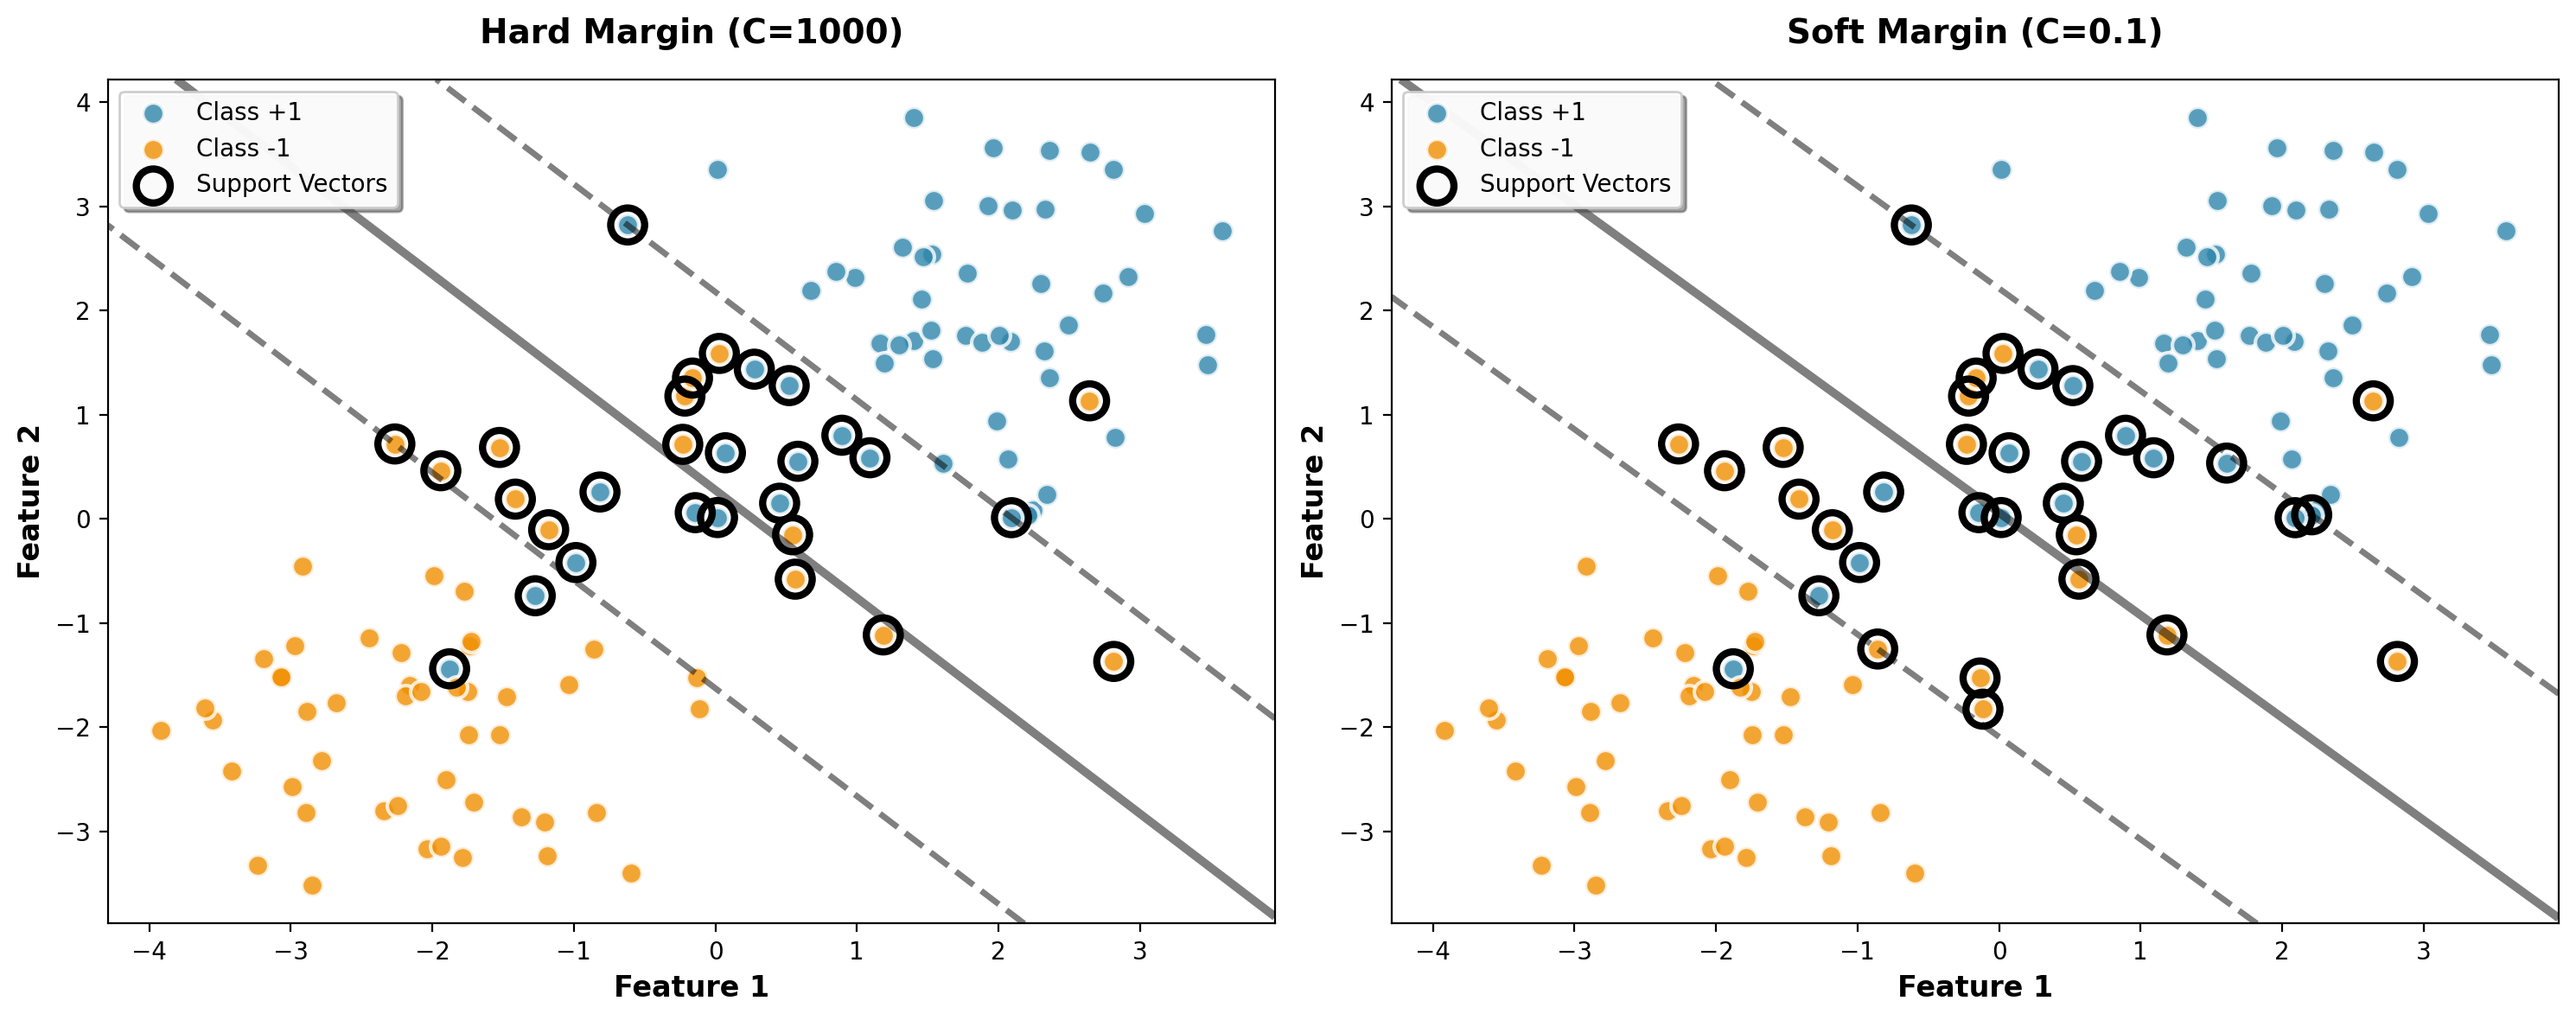
\includegraphics[width=0.9\textwidth]{../figures/hard_vs_soft_margin.png}
\end{center}

\begin{columns}[t]
\begin{column}{0.48\textwidth}
\begin{block}{Hard Margin (C = 1000)}
\begin{itemize}
\setlength{\itemsep}{1pt}
\item No training errors allowed
\item Requires linearly separable data
\item May overfit to training data
\item Complex decision boundary
\end{itemize}
\end{block}
\end{column}

\begin{column}{0.48\textwidth}
\begin{block}{Soft Margin (C = 0.1)}
\begin{itemize}
\setlength{\itemsep}{1pt}
\item Allows some training errors
\item Works with non-separable data
\item Better generalization
\item Smoother decision boundary
\end{itemize}
\end{block}
\end{column}
\end{columns}
\end{frame}

\section{Nonlinear SVM using Kernels}

\begin{frame}{The Kernel Trick}
\begin{columns}[t]
\begin{column}{0.48\textwidth}
\textbf{Feature Mapping:}
\vspace{0.2cm}

Transform input space $\mathcal{X}$ to feature space $\mathcal{H}$:
$$\phi: \mathcal{X} \rightarrow \mathcal{H}$$

\vspace{0.3cm}
\textbf{Example: Polynomial Features}
\begin{align}
x &= (x_1, x_2) \\
\phi(x) &= (1, x_1, x_2, x_1^2, x_2^2, \sqrt{2}x_1 x_2)
\end{align}

\vspace{0.3cm}
\begin{block}{Kernel Function}
Instead of computing $\phi(x_i)^T \phi(x_j)$ explicitly:
$$K(x_i, x_j) = \phi(x_i)^T \phi(x_j)$$
\end{block}

\vspace{0.3cm}
\begin{alertblock}{Key Insight}
We can compute inner products in high-dimensional space without explicitly mapping to that space!
\end{alertblock}
\end{column}

\begin{column}{0.48\textwidth}
\textbf{Computational Advantage:}
\vspace{0.2cm}

\textbf{Without Kernel Trick:}
\begin{itemize}
\setlength{\itemsep}{1pt}
\item Map: $\mathcal{O}(d')$ where $d'$ is feature space dimension
\item Inner product: $\mathcal{O}(d')$
\item Total: $\mathcal{O}(d')$ per pair
\end{itemize}

\vspace{0.3cm}
\textbf{With Kernel Trick:}
\begin{itemize}
\setlength{\itemsep}{1pt}
\item Direct kernel computation: $\mathcal{O}(d)$ where $d$ is input dimension
\item No explicit mapping needed
\item Total: $\mathcal{O}(d)$ per pair
\end{itemize}

\vspace{0.3cm}
\textbf{Example: Polynomial Kernel}
\begin{align}
K(x, x') &= (x^T x' + 1)^2 \\
&= 1 + 2x^T x' + (x^T x')^2
\end{align}

This implicitly computes inner product in a $(d+1)(d+2)/2$ dimensional space using only $\mathcal{O}(d)$ operations!
\end{column}
\end{columns}
\end{frame}

\begin{frame}{Kernel Trick Visualization}
\begin{center}
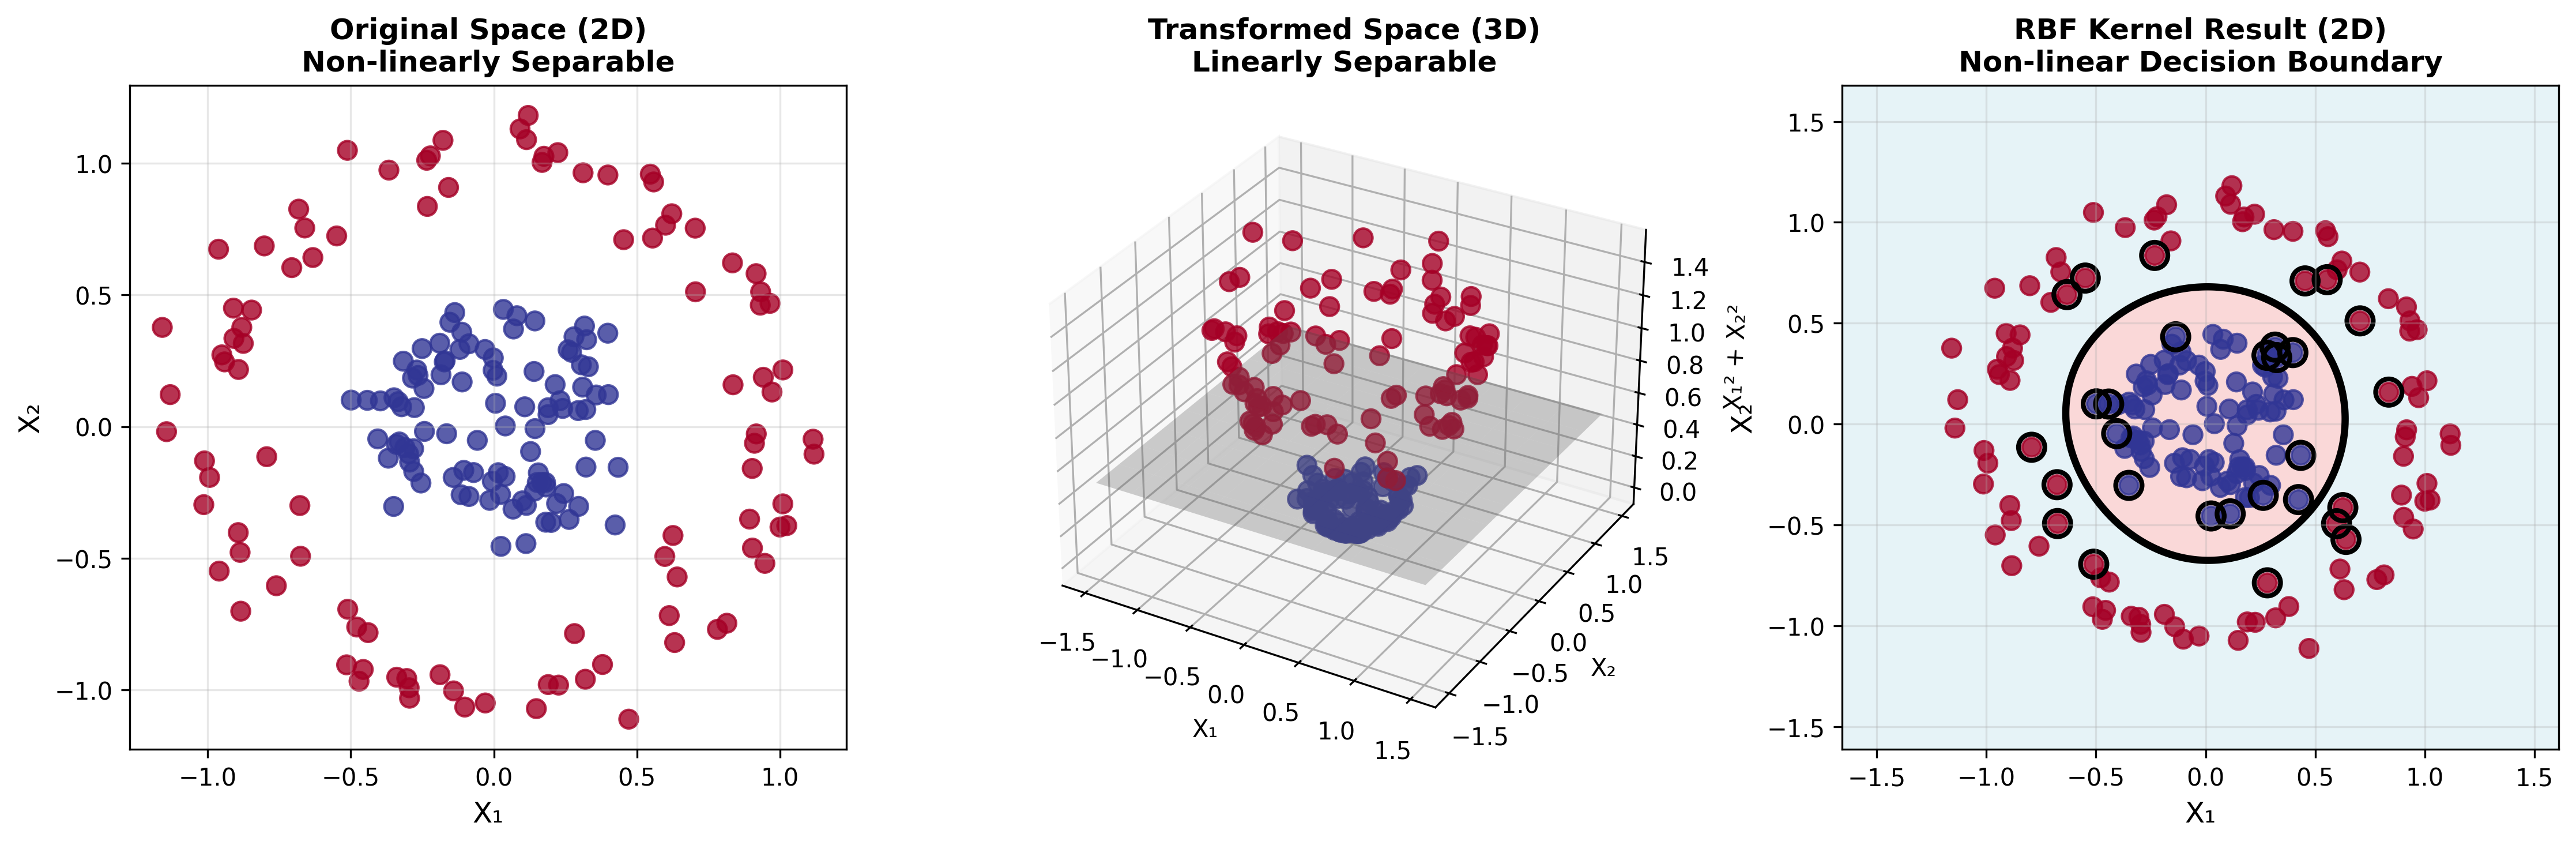
\includegraphics[width=\textwidth]{../figures/kernel_trick_transformation.png}
\end{center}

\begin{columns}[t]
\begin{column}{0.32\textwidth}
\begin{alertblock}{Original Space}
Non-linearly separable data in 2D cannot be separated by a straight line.
\end{alertblock}
\end{column}

\begin{column}{0.32\textwidth}
\begin{alertblock}{Transformed Space}
Data becomes linearly separable in 3D after polynomial transformation $\phi(x) = (x_1, x_2, x_1^2 + x_2^2)$.
\end{alertblock}
\end{column}

\begin{column}{0.32\textwidth}
\begin{alertblock}{Kernel Result}
RBF kernel achieves non-linear separation directly in original 2D space.
\end{alertblock}
\end{column}
\end{columns}
\end{frame}

\begin{frame}{Common Kernel Functions}
\begin{center}
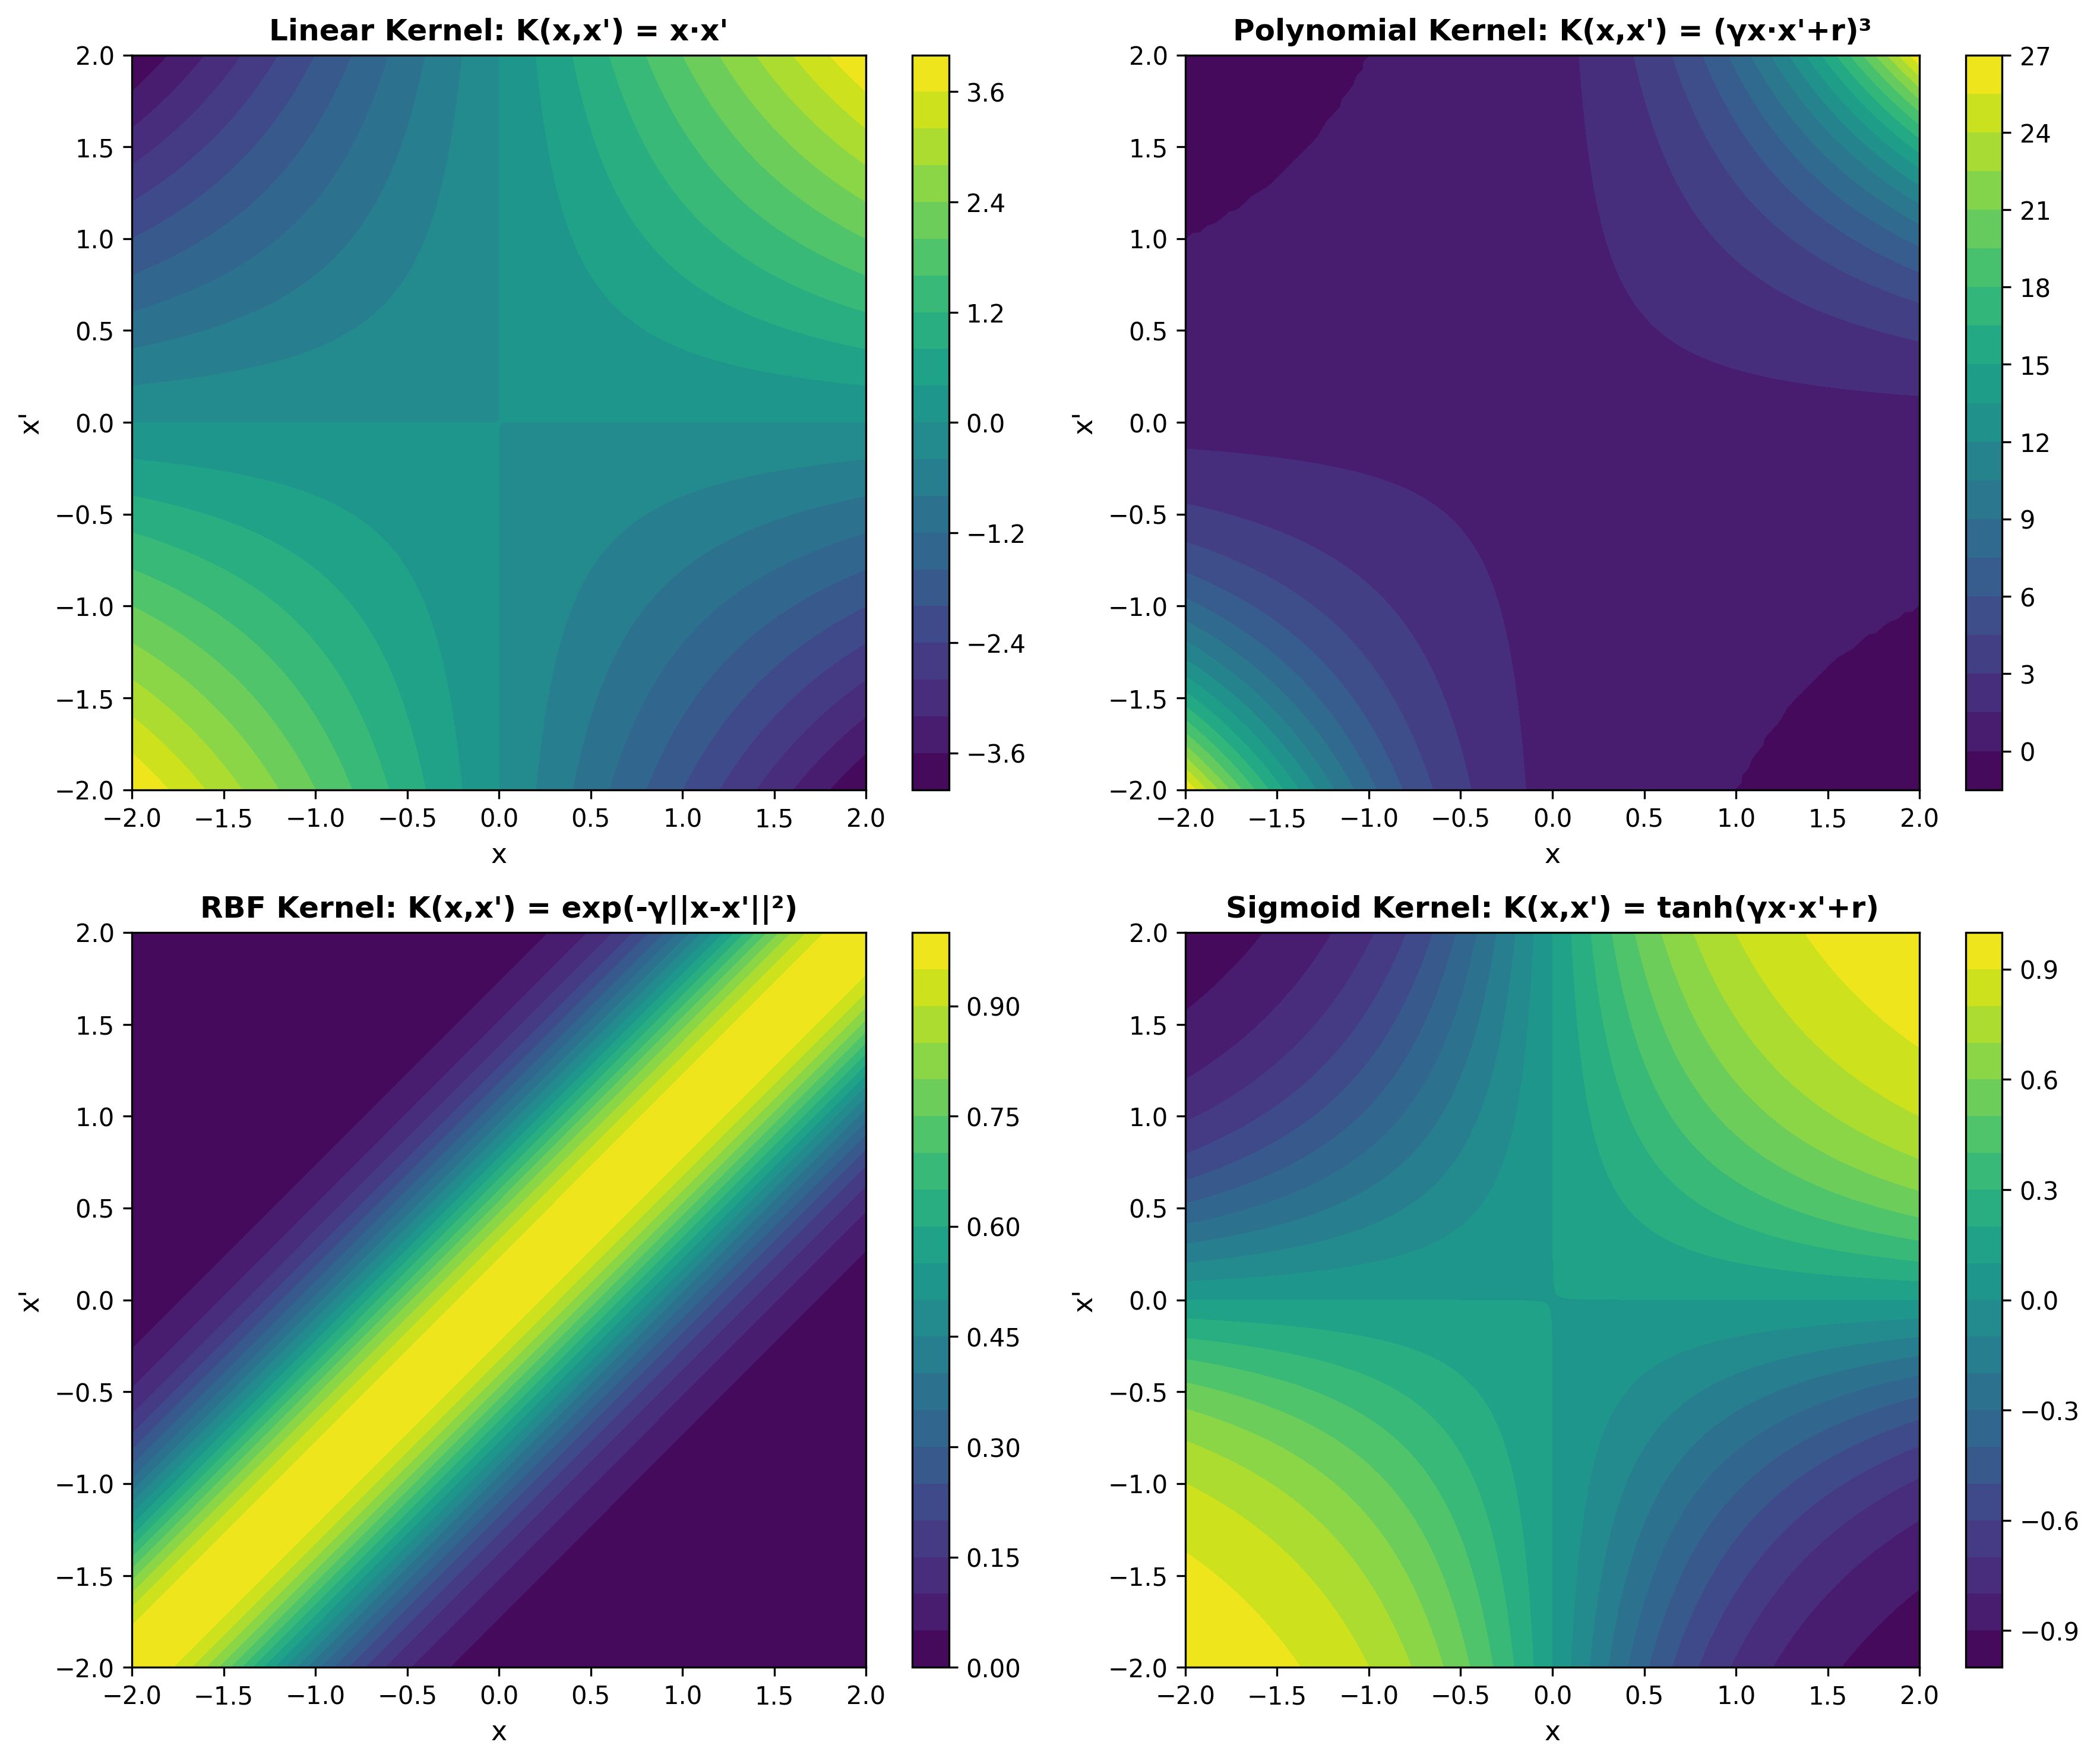
\includegraphics[width=0.9\textwidth]{../figures/kernel_functions.png}
\end{center}

\begin{columns}[t]
\begin{column}{0.48\textwidth}
\begin{block}{Linear Kernel}
$$K(x, x') = x^T x'$$
\begin{itemize}
\setlength{\itemsep}{1pt}
\item Equivalent to no transformation
\item Fastest computation
\item Good baseline
\end{itemize}
\end{block}

\begin{block}{Polynomial Kernel}
$$K(x, x') = (\gamma x^T x' + r)^d$$
\begin{itemize}
\setlength{\itemsep}{1pt}
\item Captures interactions up to degree $d$
\item Parameters: $\gamma, r, d$
\item Can model complex boundaries
\end{itemize}
\end{block}
\end{column}

\begin{column}{0.48\textwidth}
\begin{block}{RBF (Gaussian) Kernel}
$$K(x, x') = \exp\left(-\gamma \|x - x'\|^2\right)$$
\begin{itemize}
\setlength{\itemsep}{1pt}
\item Most popular kernel
\item Infinite-dimensional feature space
\item Smooth, localized similarity
\end{itemize}
\end{block}

\begin{block}{Sigmoid Kernel}
$$K(x, x') = \tanh(\gamma x^T x' + r)$$
\begin{itemize}
\setlength{\itemsep}{1pt}
\item Neural network inspired
\item Not always positive definite
\item Less commonly used
\end{itemize}
\end{block}
\end{column}
\end{columns}
\end{frame}

\begin{frame}{Comparing Different Kernels}
\begin{center}
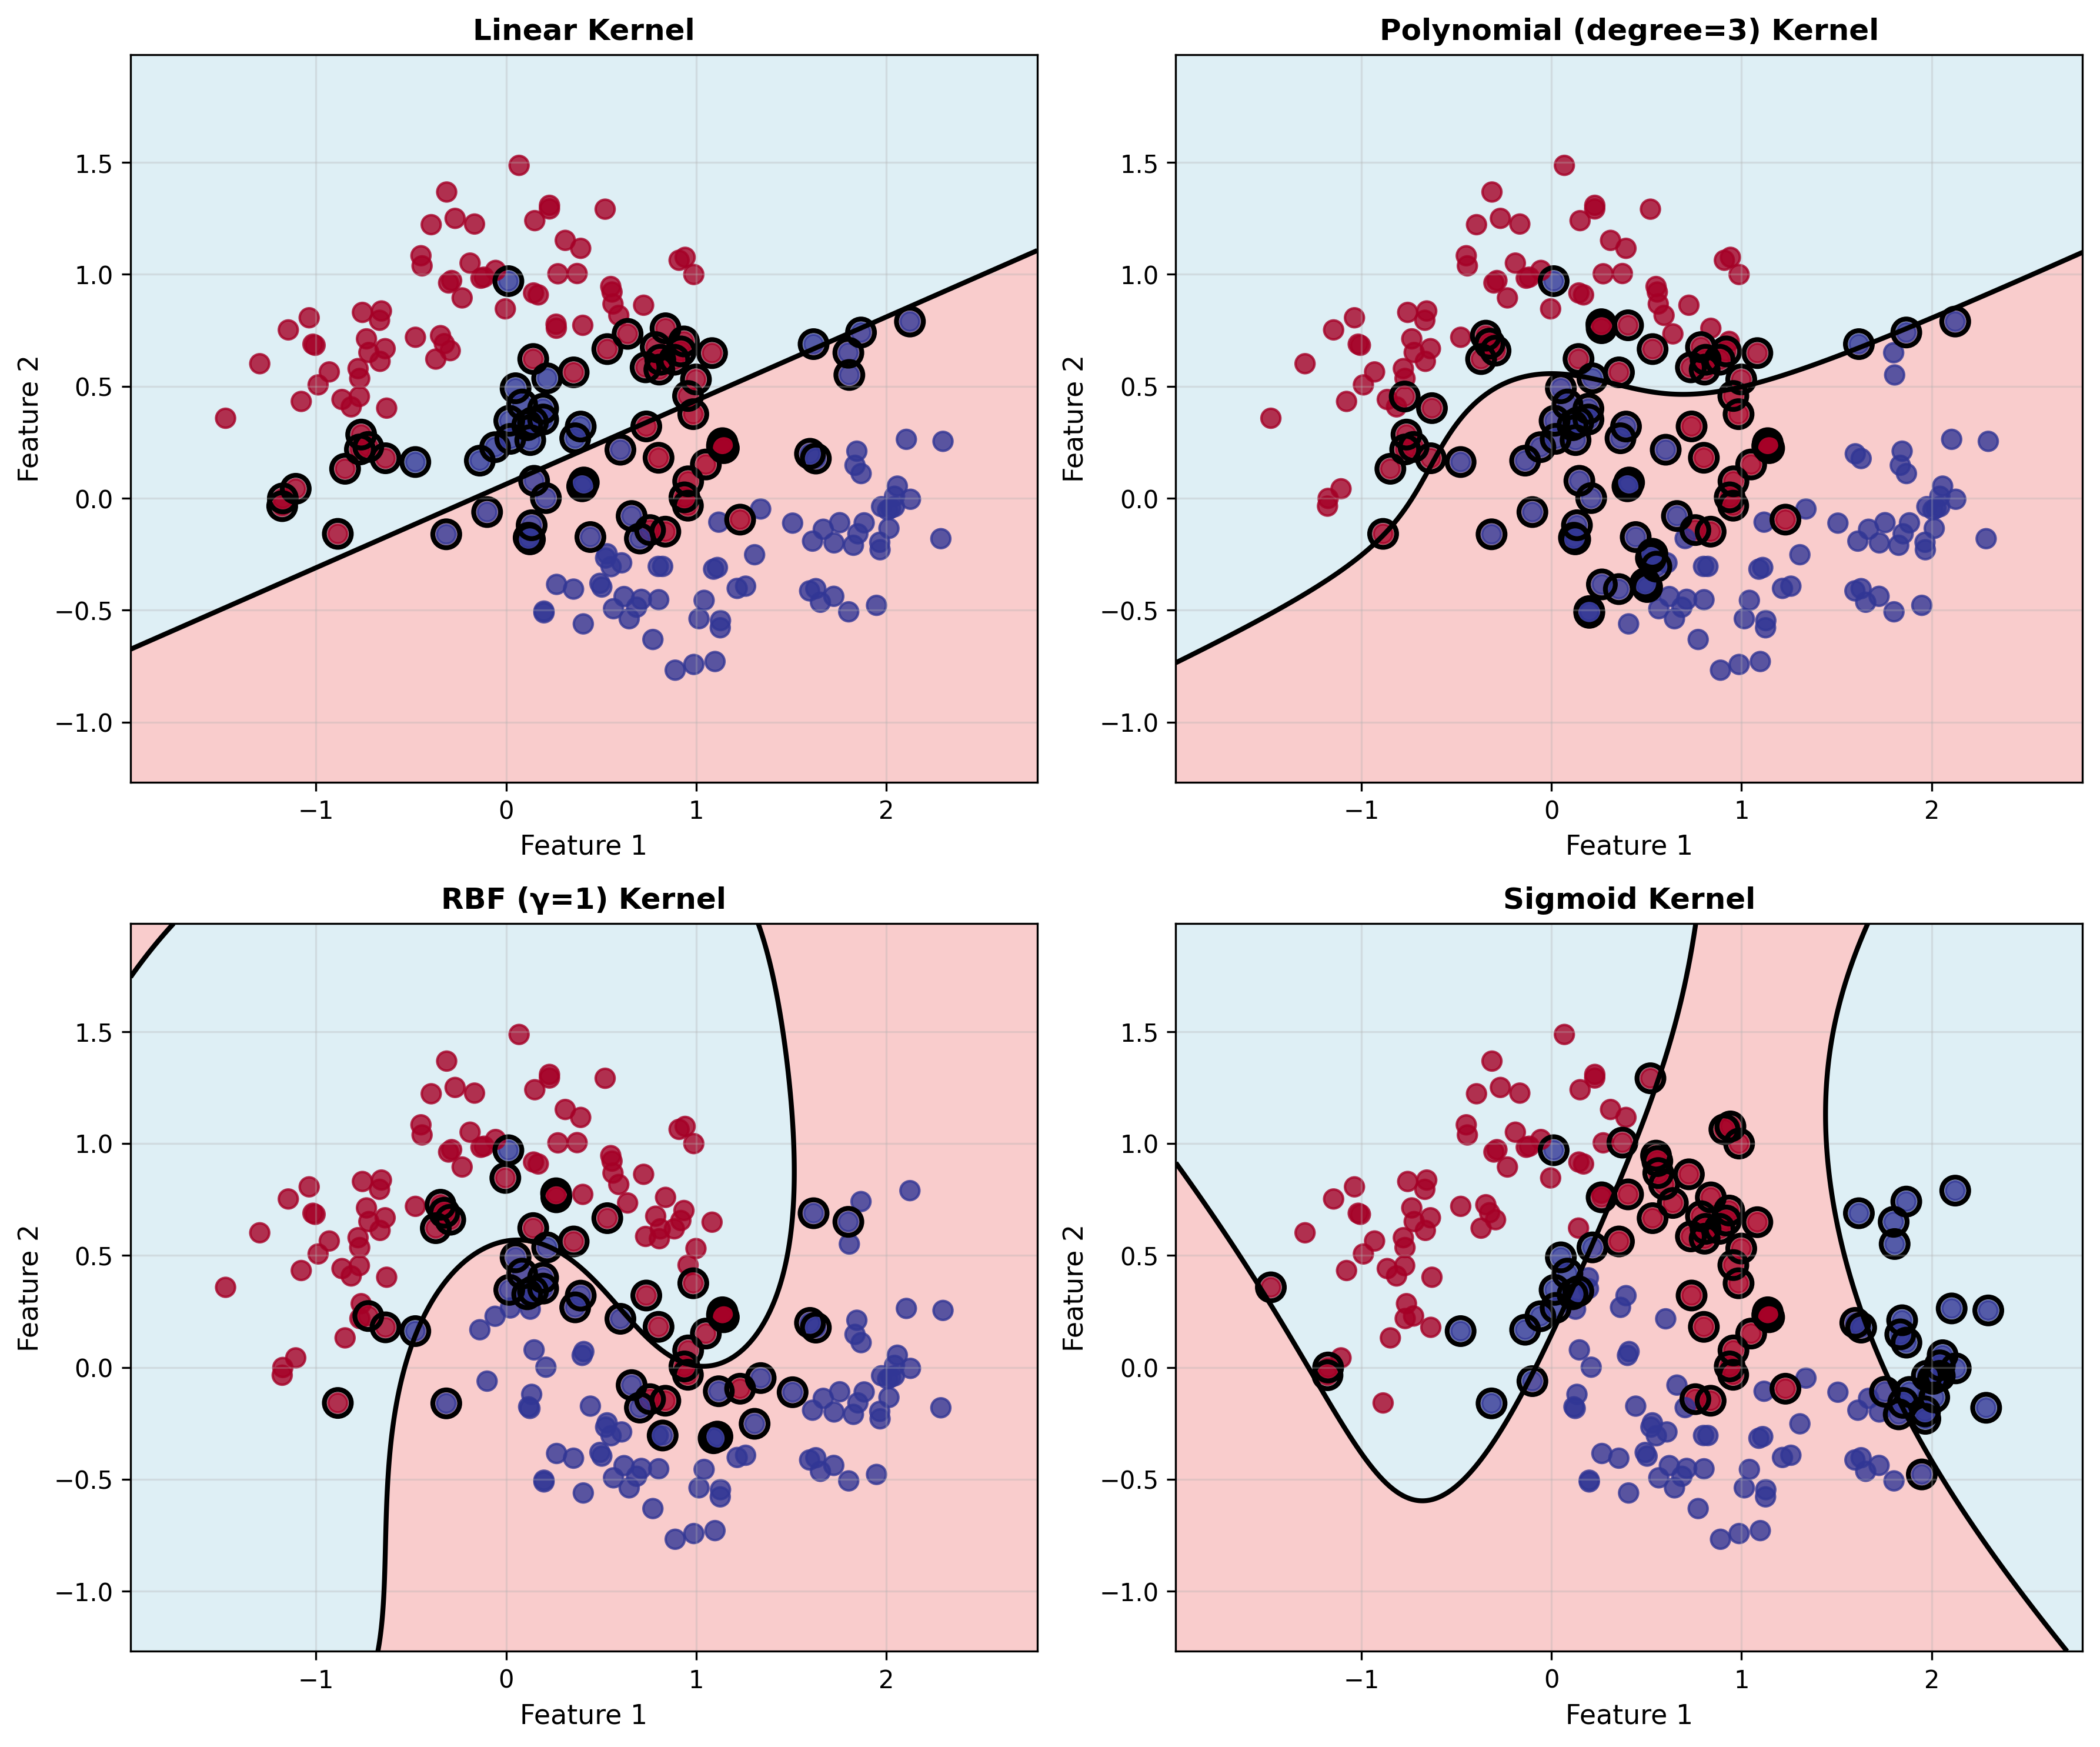
\includegraphics[width=\textwidth]{../figures/different_kernels.png}
\end{center}

\begin{columns}[t]
\begin{column}{0.48\textwidth}
\textbf{Kernel Selection Guidelines:}
\begin{itemize}
\setlength{\itemsep}{1pt}
\item \textcolor{blue}{\textbf{Linear:}} High-dimensional data, text classification
\item \textcolor{red}{\textbf{Polynomial:}} Known polynomial relationships
\item \textcolor{green}{\textbf{RBF:}} General-purpose, unknown data structure
\item \textcolor{purple}{\textbf{Sigmoid:}} Neural network replacement
\end{itemize}
\end{column}

\begin{column}{0.48\textwidth}
\textbf{Performance Factors:}
\begin{itemize}
\setlength{\itemsep}{1pt}
\item Data dimensionality
\item Training set size
\item Noise level
\item Prior domain knowledge
\item Computational constraints
\end{itemize}
\end{column}
\end{columns}
\end{frame}

\begin{frame}{RBF Kernel Parameter Effects}
\begin{center}
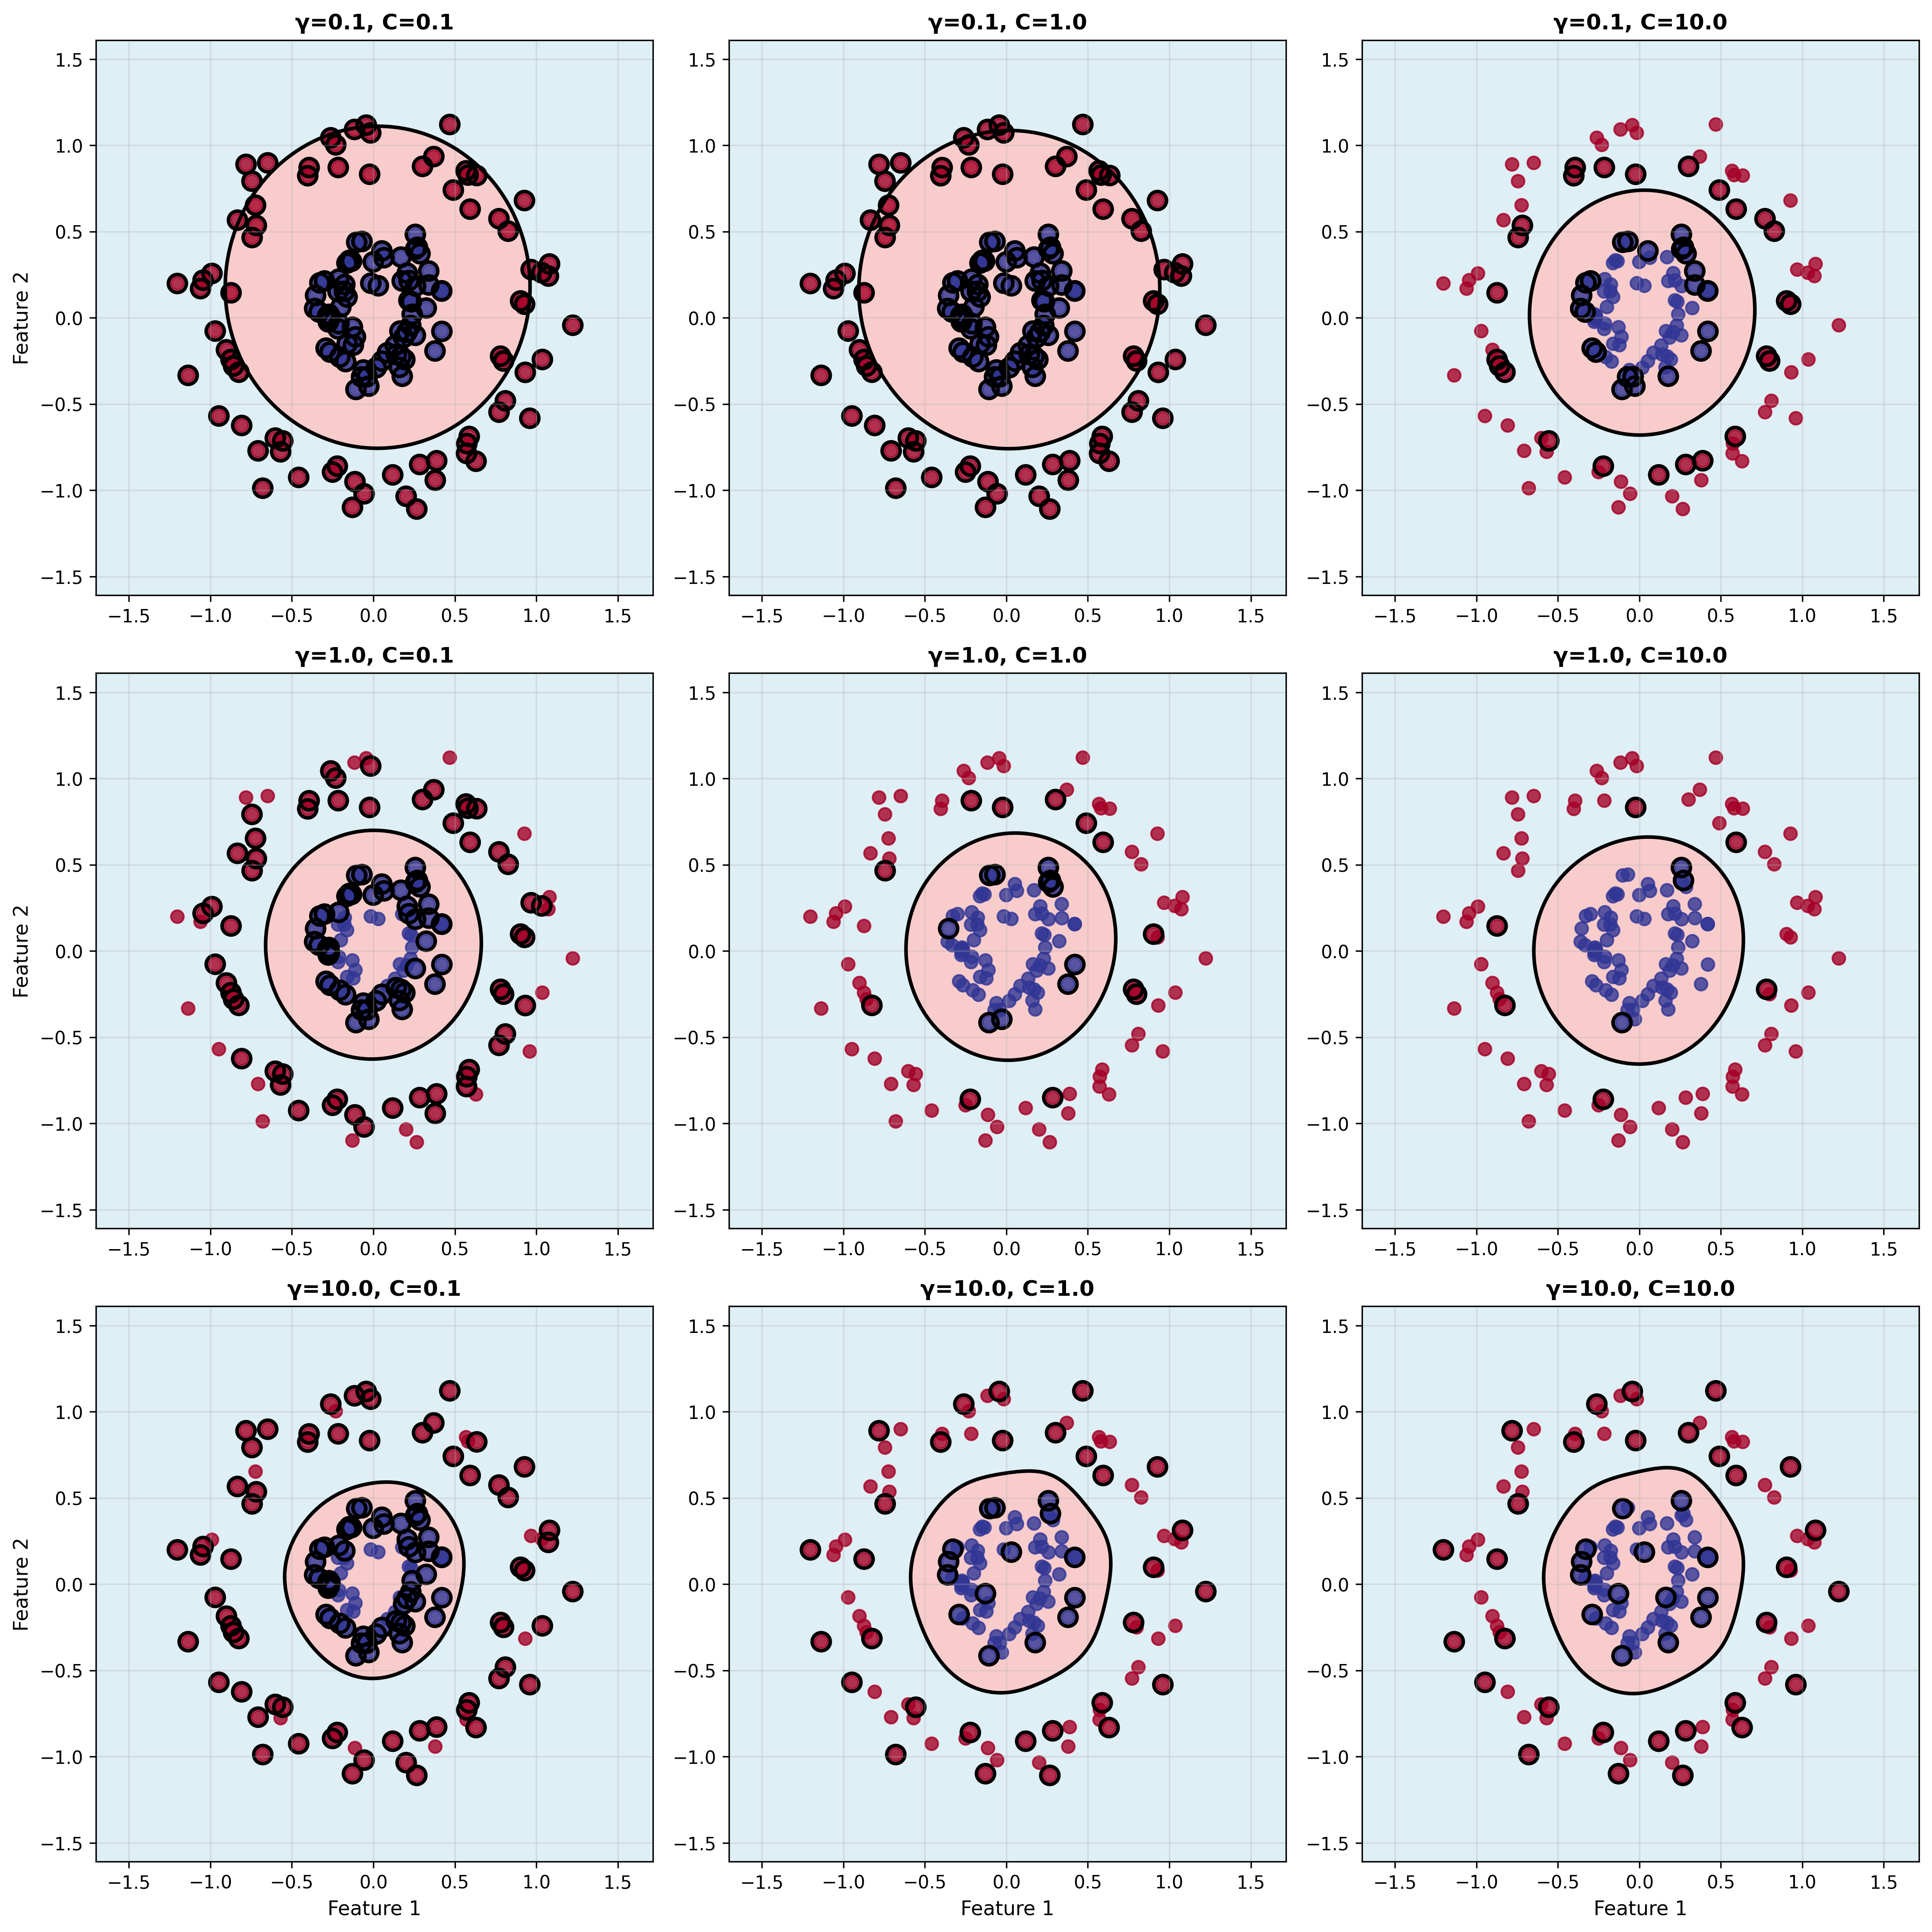
\includegraphics[width=0.85\textwidth]{../figures/rbf_kernel_parameters.png}
\end{center}

\begin{columns}[t]
\begin{column}{0.48\textwidth}
\textbf{Gamma ($\gamma$) Parameter:}
\begin{itemize}
\setlength{\itemsep}{1pt}
\item \textcolor{blue}{\textbf{Small $\gamma$:}} Wide RBF, smooth decision boundary
\item \textcolor{red}{\textbf{Large $\gamma$:}} Narrow RBF, complex boundary
\item Controls locality of influence
\end{itemize}
\end{column}

\begin{column}{0.48\textwidth}
\textbf{Regularization ($C$) Parameter:}
\begin{itemize}
\setlength{\itemsep}{1pt}
\item \textcolor{green}{\textbf{Small $C$:}} Soft margin, simpler boundary
\item \textcolor{orange}{\textbf{Large $C$:}} Hard margin, complex boundary
\item Controls bias-variance tradeoff
\end{itemize}
\end{column}
\end{columns}
\end{frame}

\section{Mercer's Theorem}

\begin{frame}{Mercer's Theorem: Valid Kernels}
\begin{columns}[t]
\begin{column}{0.48\textwidth}
\begin{block}{Mercer's Theorem}
A function $K(x, x')$ is a valid kernel (corresponds to an inner product in some feature space) if and only if for any finite set of points $\{x_1, \ldots, x_n\}$, the kernel matrix $\mathbf{K}$ is positive semi-definite.
\end{block}

\vspace{0.3cm}
\textbf{Kernel Matrix:}
$$\mathbf{K}_{ij} = K(x_i, x_j)$$

\vspace{0.3cm}
\textbf{Positive Semi-definite:}
$$\mathbf{K} \succeq 0 \iff \sum_{i,j} c_i c_j K(x_i, x_j) \geq 0$$
for all real numbers $c_1, \ldots, c_n$.

\vspace{0.3cm}
\begin{alertblock}{Practical Implication}
Not every function can be used as a kernel! Only those satisfying Mercer's condition.
\end{alertblock}
\end{column}

\begin{column}{0.48\textwidth}
\textbf{Properties of Valid Kernels:}
\vspace{0.2cm}

\begin{itemize}
\setlength{\itemsep}{1pt}
\item \textbf{Symmetry:} $K(x, x') = K(x', x)$
\item \textbf{Positive semi-definiteness:} Kernel matrix $\mathbf{K} \succeq 0$
\end{itemize}

\vspace{0.3cm}
\textbf{Constructing New Kernels:}
\vspace{0.2cm}

If $K_1$ and $K_2$ are valid kernels, then:
\begin{align}
K(x, x') &= K_1(x, x') + K_2(x, x') \\
K(x, x') &= c \cdot K_1(x, x'), \quad c > 0 \\
K(x, x') &= K_1(x, x') \cdot K_2(x, x') \\
K(x, x') &= \exp(K_1(x, x')) \\
K(x, x') &= f(x) K_1(x, x') f(x')
\end{align}

\vspace{0.3cm}
\textbf{Domain-Specific Kernels:}
\begin{itemize}
\setlength{\itemsep}{1pt}
\item String kernels for text
\item Graph kernels for networks
\item Tree kernels for structured data
\end{itemize}
\end{column}
\end{columns}
\end{frame}

\begin{frame}{Examples of Valid and Invalid Kernels}
\begin{columns}[t]
\begin{column}{0.48\textwidth}
\textbf{Valid Kernels:}
\vspace{0.2cm}

\begin{block}{Linear}
$$K(x, x') = x^T x'$$
\end{block}

\begin{block}{Polynomial}
$$K(x, x') = (x^T x' + 1)^d, \quad d \geq 1$$
\end{block}

\begin{block}{RBF/Gaussian}
$$K(x, x') = \exp\left(-\frac{\|x - x'\|^2}{2\sigma^2}\right)$$
\end{block}

\begin{block}{Exponential}
$$K(x, x') = \exp(-\gamma \|x - x'\|), \quad \gamma > 0$$
\end{block}

\vspace{0.3cm}
\textbf{Why Valid?}
All can be shown to correspond to inner products in (possibly infinite-dimensional) feature spaces.
\end{column}

\begin{column}{0.48\textwidth}
\textbf{Invalid Kernels:}
\vspace{0.2cm}

\begin{block}{Negative Power}
$$K(x, x') = (x^T x')^{-1}$$
Not positive semi-definite.
\end{block}

\begin{block}{Logarithmic}
$$K(x, x') = \log(x^T x' + 1)$$
Can produce negative eigenvalues.
\end{block}

\vspace{0.3cm}
\textbf{Checking Validity:}
\vspace{0.2cm}

\begin{enumerate}
\setlength{\itemsep}{1pt}
\item \textbf{Theoretical:} Prove positive semi-definiteness
\item \textbf{Computational:} Check eigenvalues of kernel matrix
\item \textbf{Construction:} Build from known valid kernels
\end{enumerate}

\vspace{0.3cm}
\begin{alertblock}{Practical Note}
Most standard kernels in ML libraries are guaranteed to be valid. Custom kernels need verification.
\end{alertblock}
\end{column}
\end{columns}
\end{frame}

\section{Multiple Kernel Learning}

\begin{frame}{Multiple Kernel Learning (MKL)}
\begin{columns}[t]
\begin{column}{0.48\textwidth}
\begin{block}{Motivation}
Different kernels capture different aspects of data:
\begin{itemize}
\setlength{\itemsep}{1pt}
\item RBF kernel: local similarities
\item Linear kernel: global structure
\item Polynomial kernel: feature interactions
\end{itemize}
\end{block}

\vspace{0.3cm}
\textbf{Idea:} Combine multiple kernels to get better performance than any single kernel.

\vspace{0.3cm}
\textbf{Linear Combination:}
$$K(x, x') = \sum_{m=1}^M \beta_m K_m(x, x')$$

where $\beta_m \geq 0$ and $\sum_{m=1}^M \beta_m = 1$.

\vspace{0.3cm}
\textbf{Applications:}
\begin{itemize}
\setlength{\itemsep}{1pt}
\item Multi-modal data (text + images)
\item Feature selection
\item Domain adaptation
\end{itemize}
\end{column}

\begin{column}{0.48\textwidth}
\textbf{MKL Optimization:}
\vspace{0.2cm}

\begin{block}{Joint Optimization}
\begin{align}
\min_{w,b,\xi,\beta} \quad &\frac{1}{2}\sum_{m=1}^M \frac{\|w_m\|^2}{\beta_m} + C\sum_{i=1}^n \xi_i \\
\text{subject to} \quad &y_i\left(\sum_{m=1}^M w_m^T \phi_m(x_i) + b\right) \geq 1 - \xi_i \\
&\xi_i \geq 0, \quad \beta_m \geq 0, \quad \sum_{m=1}^M \beta_m = 1
\end{align}
\end{block}

\vspace{0.3cm}
\textbf{Solution Methods:}
\begin{itemize}
\setlength{\itemsep}{1pt}
\item \textbf{Alternating optimization:} Fix $\beta$, solve for $w$; fix $w$, solve for $\beta$
\item \textbf{Semi-definite programming:} Convex formulation
\item \textbf{Gradient-based methods:} Efficient for large-scale
\end{itemize}

\vspace{0.3cm}
\textbf{Kernel Weight Interpretation:}
\begin{itemize}
\setlength{\itemsep}{1pt}
\item $\beta_m$ close to 1: Kernel $m$ is most important
\item $\beta_m$ close to 0: Kernel $m$ is irrelevant
\item Automatic feature/kernel selection
\end{itemize}
\end{column}
\end{columns}
\end{frame}

\begin{frame}{MKL Example: Combining Kernels}
\begin{columns}[t]
\begin{column}{0.48\textwidth}
\textbf{Example Setup:}
\vspace{0.2cm}

Consider combining three kernels:
\begin{align}
K_1(x, x') &= x^T x' \quad \text{(Linear)} \\
K_2(x, x') &= (x^T x' + 1)^2 \quad \text{(Polynomial)} \\
K_3(x, x') &= \exp(-\|x-x'\|^2) \quad \text{(RBF)}
\end{align}

\vspace{0.3cm}
\textbf{Combined Kernel:}
$$K(x, x') = \beta_1 K_1(x, x') + \beta_2 K_2(x, x') + \beta_3 K_3(x, x')$$

\vspace{0.3cm}
\textbf{Learning Process:}
\begin{enumerate}
\setlength{\itemsep}{1pt}
\item Start with equal weights: $\beta_1 = \beta_2 = \beta_3 = \frac{1}{3}$
\item Iteratively optimize weights and SVM parameters
\item Converge to optimal combination
\end{enumerate}
\end{column}

\begin{column}{0.48\textwidth}
\textbf{Sample Results:}
\vspace{0.2cm}

\begin{center}
\begin{tabular}{|l|c|c|}
\hline
\textbf{Kernel} & \textbf{Weight} & \textbf{Accuracy} \\
\hline
Linear & 0.1 & 0.78 \\
Polynomial & 0.3 & 0.82 \\
RBF & 0.6 & 0.85 \\
\hline
\textbf{Combined MKL} & \textbf{-} & \textbf{0.89} \\
\hline
\end{tabular}
\end{center}

\vspace{0.3cm}
\textbf{Advantages:}
\begin{itemize}
\setlength{\itemsep}{1pt}
\item \textcolor{green}{\textbf{Better performance}} than individual kernels
\item \textcolor{blue}{\textbf{Automatic selection}} of relevant kernels
\item \textcolor{purple}{\textbf{Interpretability}} through weights
\end{itemize}

\vspace{0.3cm}
\textbf{Challenges:}
\begin{itemize}
\setlength{\itemsep}{1pt}
\item Increased computational complexity
\item More hyperparameters to tune
\item Risk of overfitting with many kernels
\end{itemize}
\end{column}
\end{columns}
\end{frame}

\section{Multi-class Classification}

\begin{frame}{Multi-class SVM Strategies}
\begin{center}
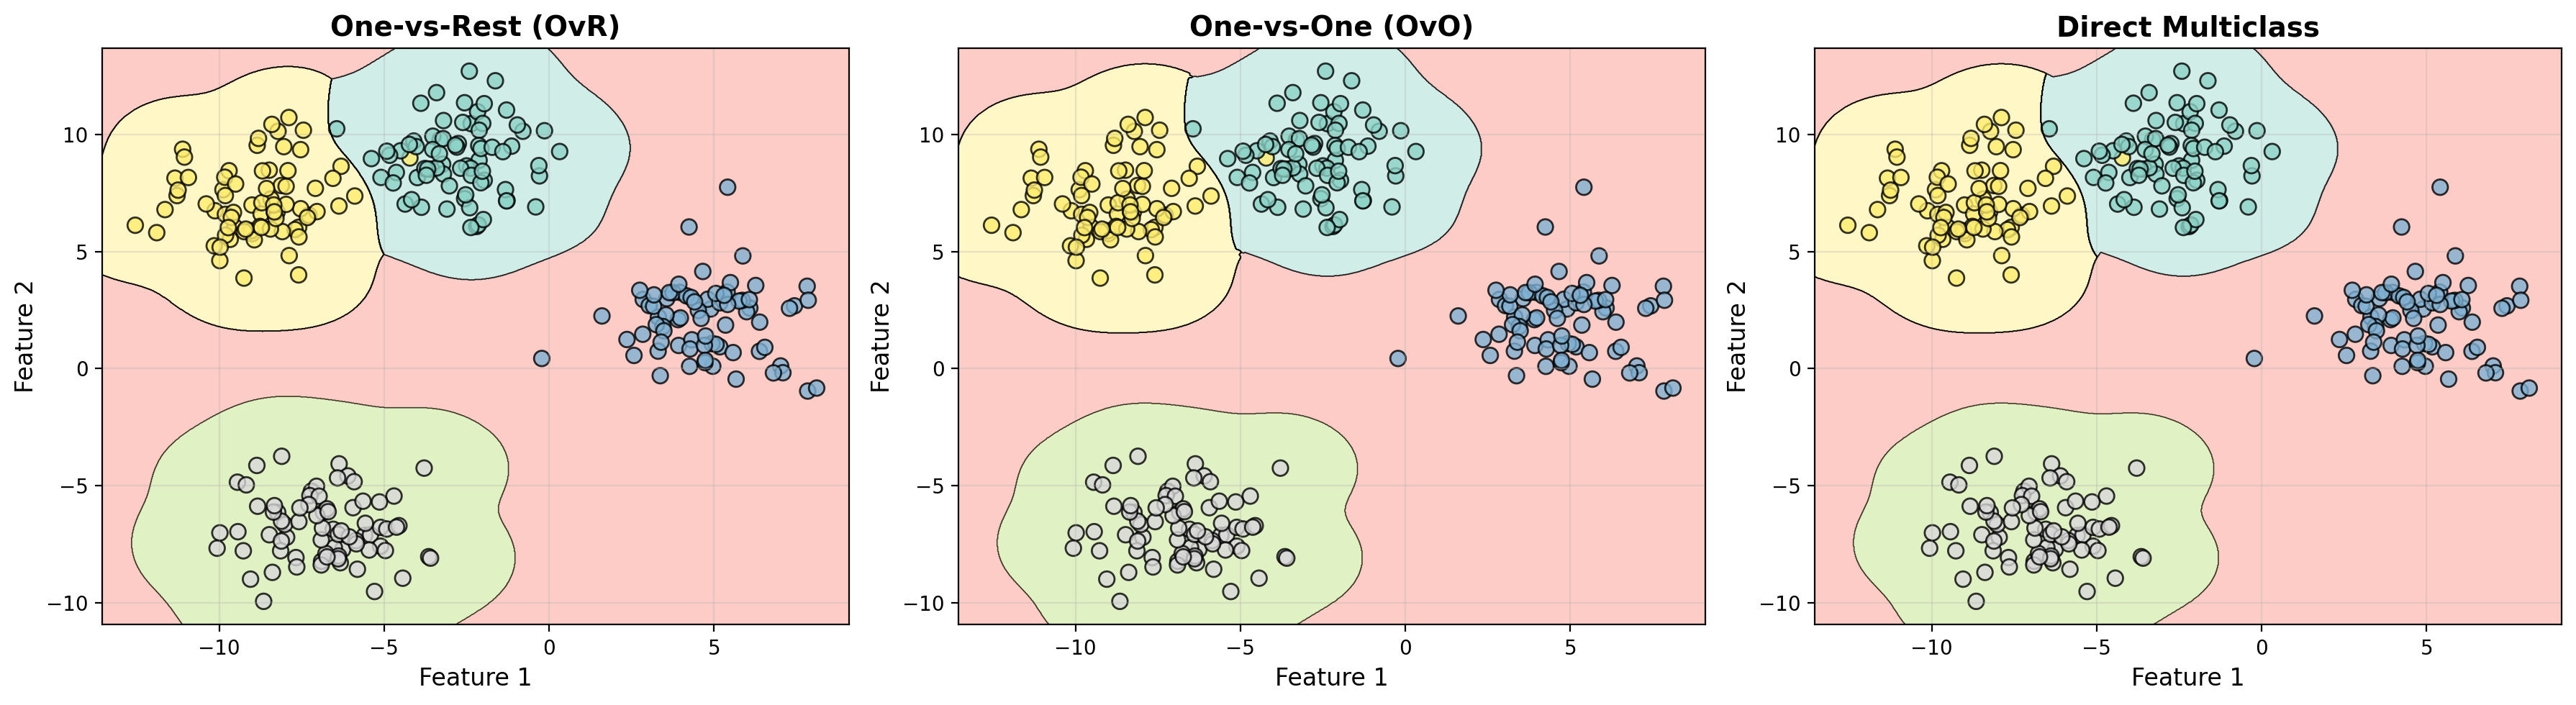
\includegraphics[width=\textwidth]{../figures/multiclass_strategies.png}
\end{center}

\begin{columns}[t]
\begin{column}{0.32\textwidth}
\begin{block}{One-vs-Rest (OvR)}
\begin{itemize}
\setlength{\itemsep}{1pt}
\item Train $k$ binary classifiers
\item Each separates one class from all others
\item Prediction: class with highest score
\end{itemize}
\end{block}
\end{column}

\begin{column}{0.32\textwidth}
\begin{block}{One-vs-One (OvO)}
\begin{itemize}
\setlength{\itemsep}{1pt}
\item Train $\binom{k}{2}$ binary classifiers
\item Each separates pair of classes
\item Prediction: majority voting
\end{itemize}
\end{block}
\end{column}

\begin{column}{0.32\textwidth}
\begin{block}{Direct Multiclass}
\begin{itemize}
\setlength{\itemsep}{1pt}
\item Single optimization problem
\item Simultaneous separation
\item More complex but unified
\end{itemize}
\end{block}
\end{column}
\end{columns}
\end{frame}

\begin{frame}{One-vs-Rest Detailed Analysis}
\begin{center}
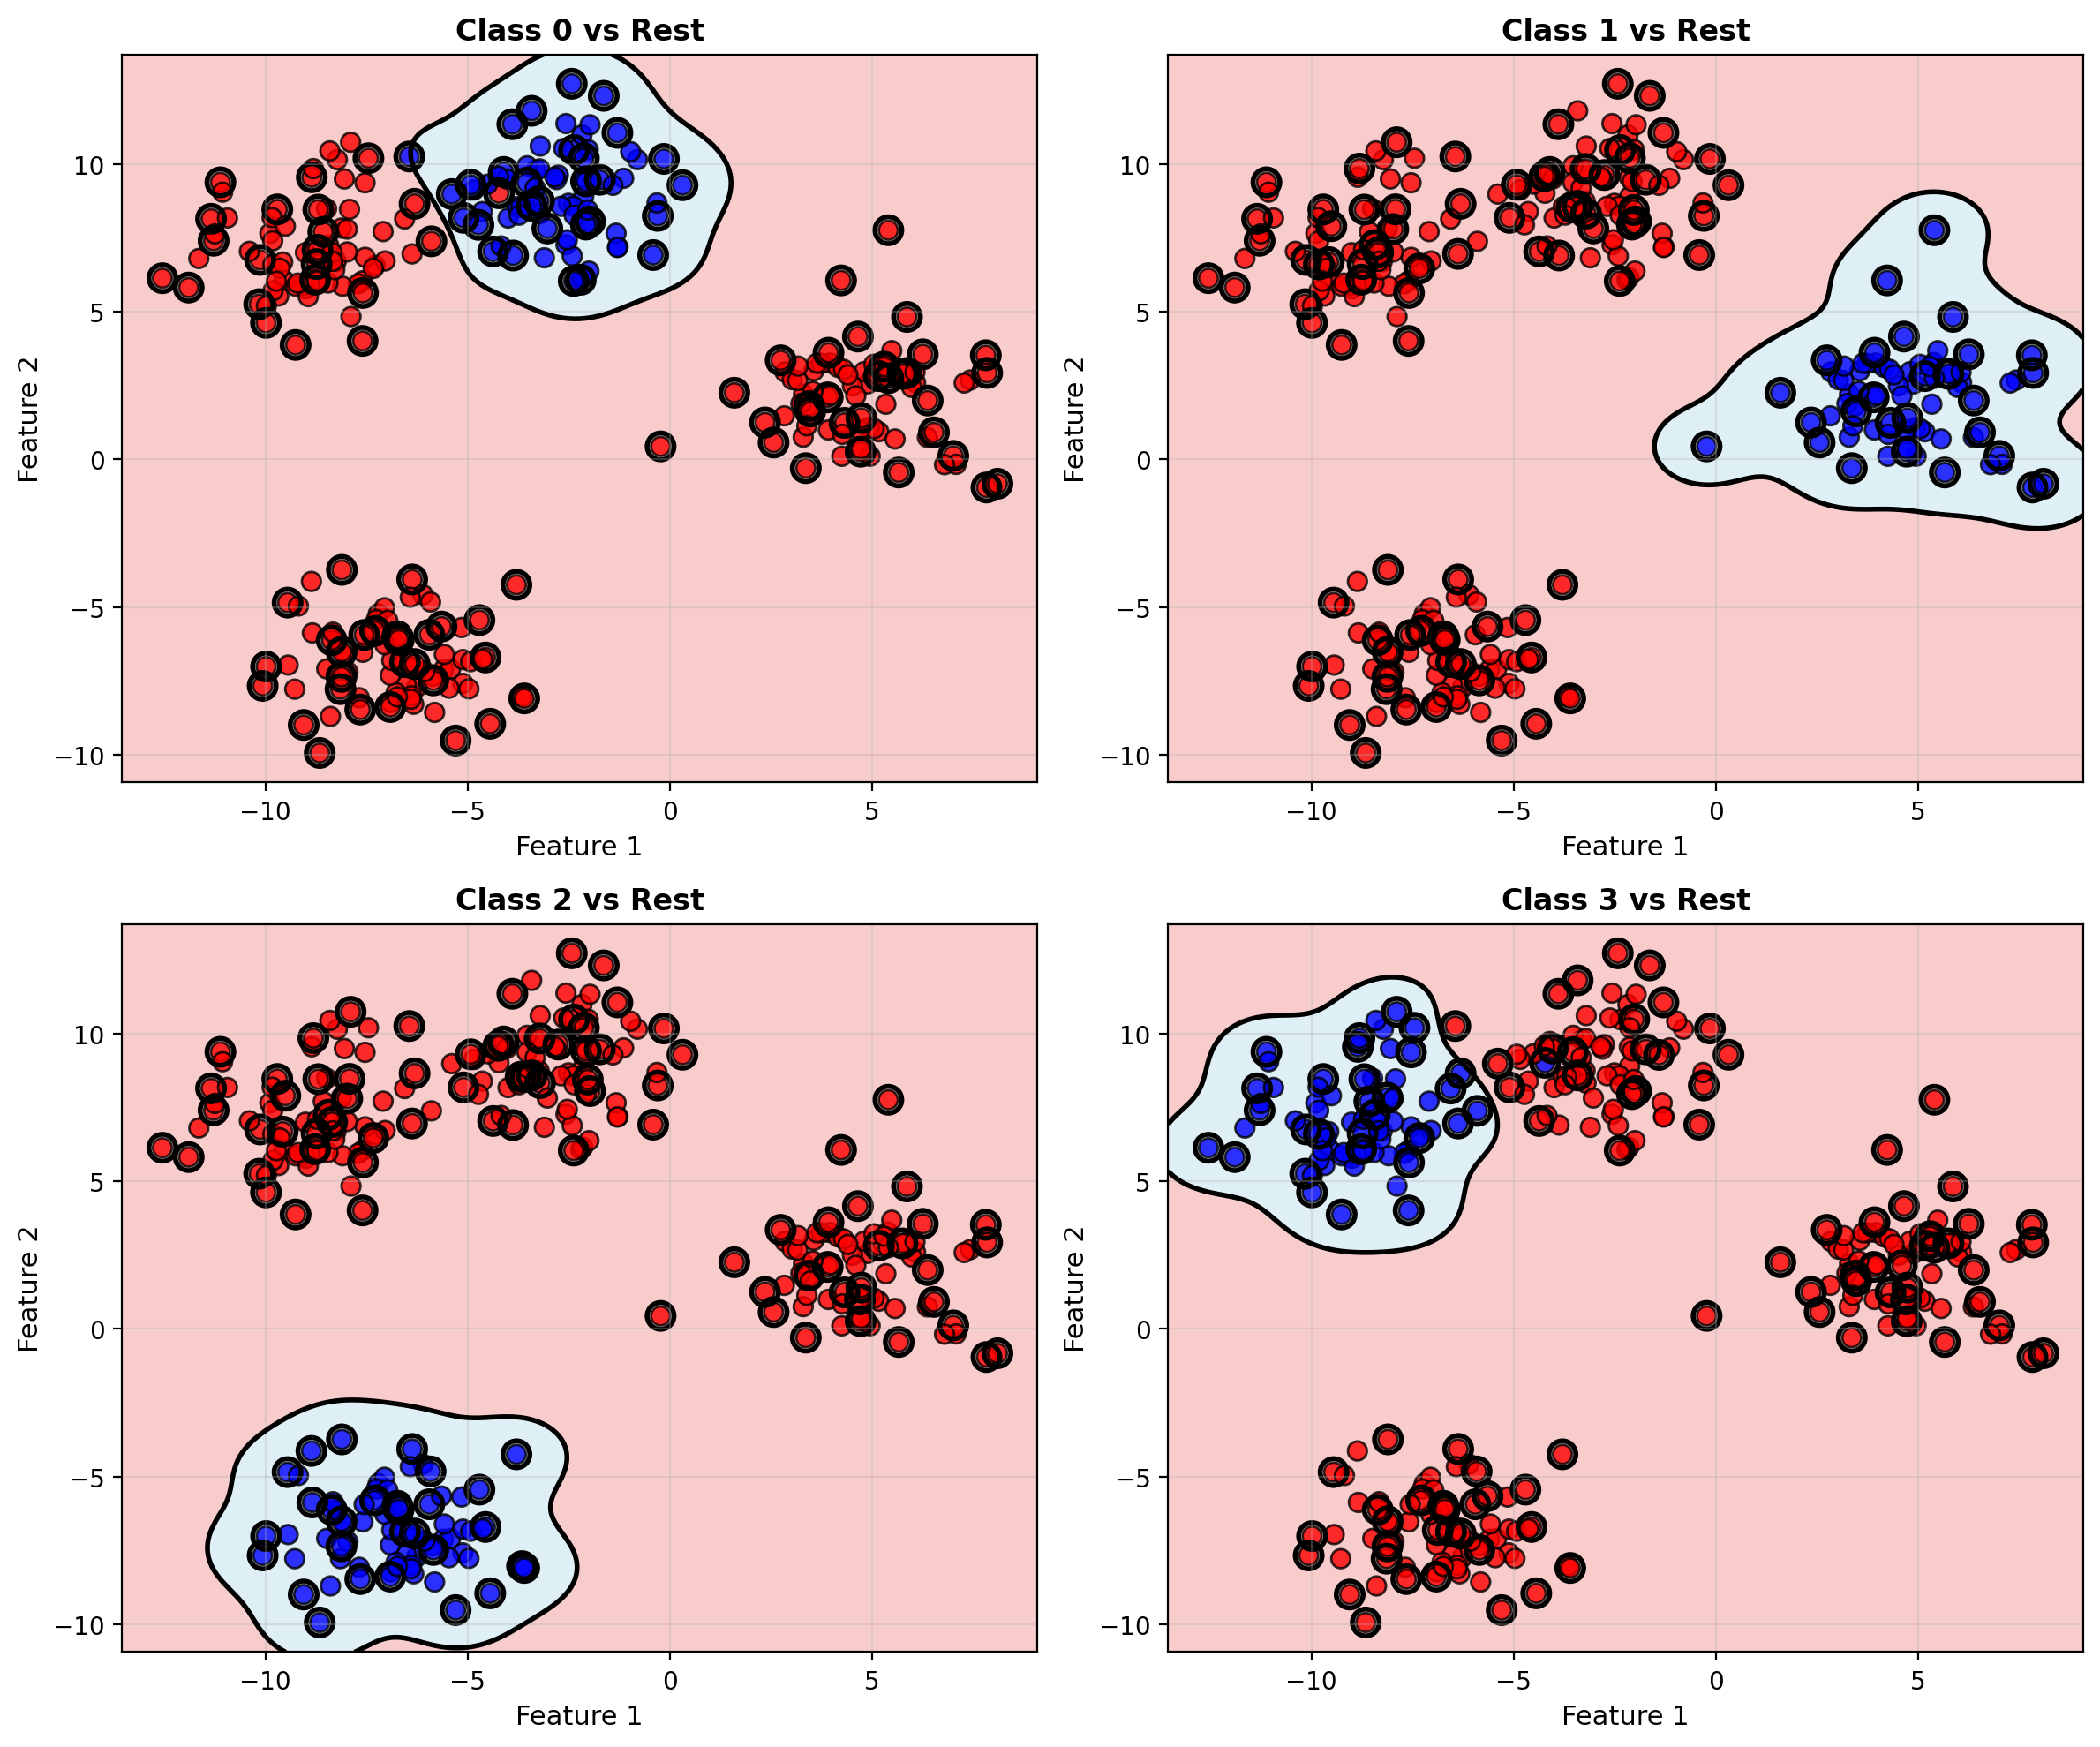
\includegraphics[width=0.9\textwidth]{../figures/ovr_detailed.png}
\end{center}

\begin{columns}[t]
\begin{column}{0.48\textwidth}
\textbf{OvR Strategy:}
\vspace{0.2cm}

For $k$-class problem:
\begin{enumerate}
\setlength{\itemsep}{1pt}
\item Train classifier 1: Class 0 vs {1,2,3}
\item Train classifier 2: Class 1 vs {0,2,3}
\item Train classifier 3: Class 2 vs {0,1,3}
\item Train classifier 4: Class 3 vs {0,1,2}
\end{enumerate}

\vspace{0.3cm}
\textbf{Prediction:}
$$\hat{y} = \arg\max_{j} f_j(x)$$
where $f_j(x)$ is the decision function of classifier $j$.
\end{column}

\begin{column}{0.48\textwidth}
\textbf{Advantages:}
\begin{itemize}
\setlength{\itemsep}{1pt}
\item Simple to implement
\item Training scales linearly with $k$
\item Can use any binary classifier
\item Probabilistic interpretation possible
\end{itemize}

\vspace{0.3cm}
\textbf{Disadvantages:}
\begin{itemize}
\setlength{\itemsep}{1pt}
\item Class imbalance in binary problems
\item Inconsistent decision regions
\item Ambiguous predictions possible
\end{itemize}

\vspace{0.3cm}
\textbf{Complexity:}
\begin{itemize}
\setlength{\itemsep}{1pt}
\item Training: $\mathcal{O}(k \cdot \text{binary training})$
\item Prediction: $\mathcal{O}(k \cdot \text{binary prediction})$
\end{itemize}
\end{column}
\end{columns}
\end{frame}

\begin{frame}{Multi-class Kernel Comparison}
\begin{center}
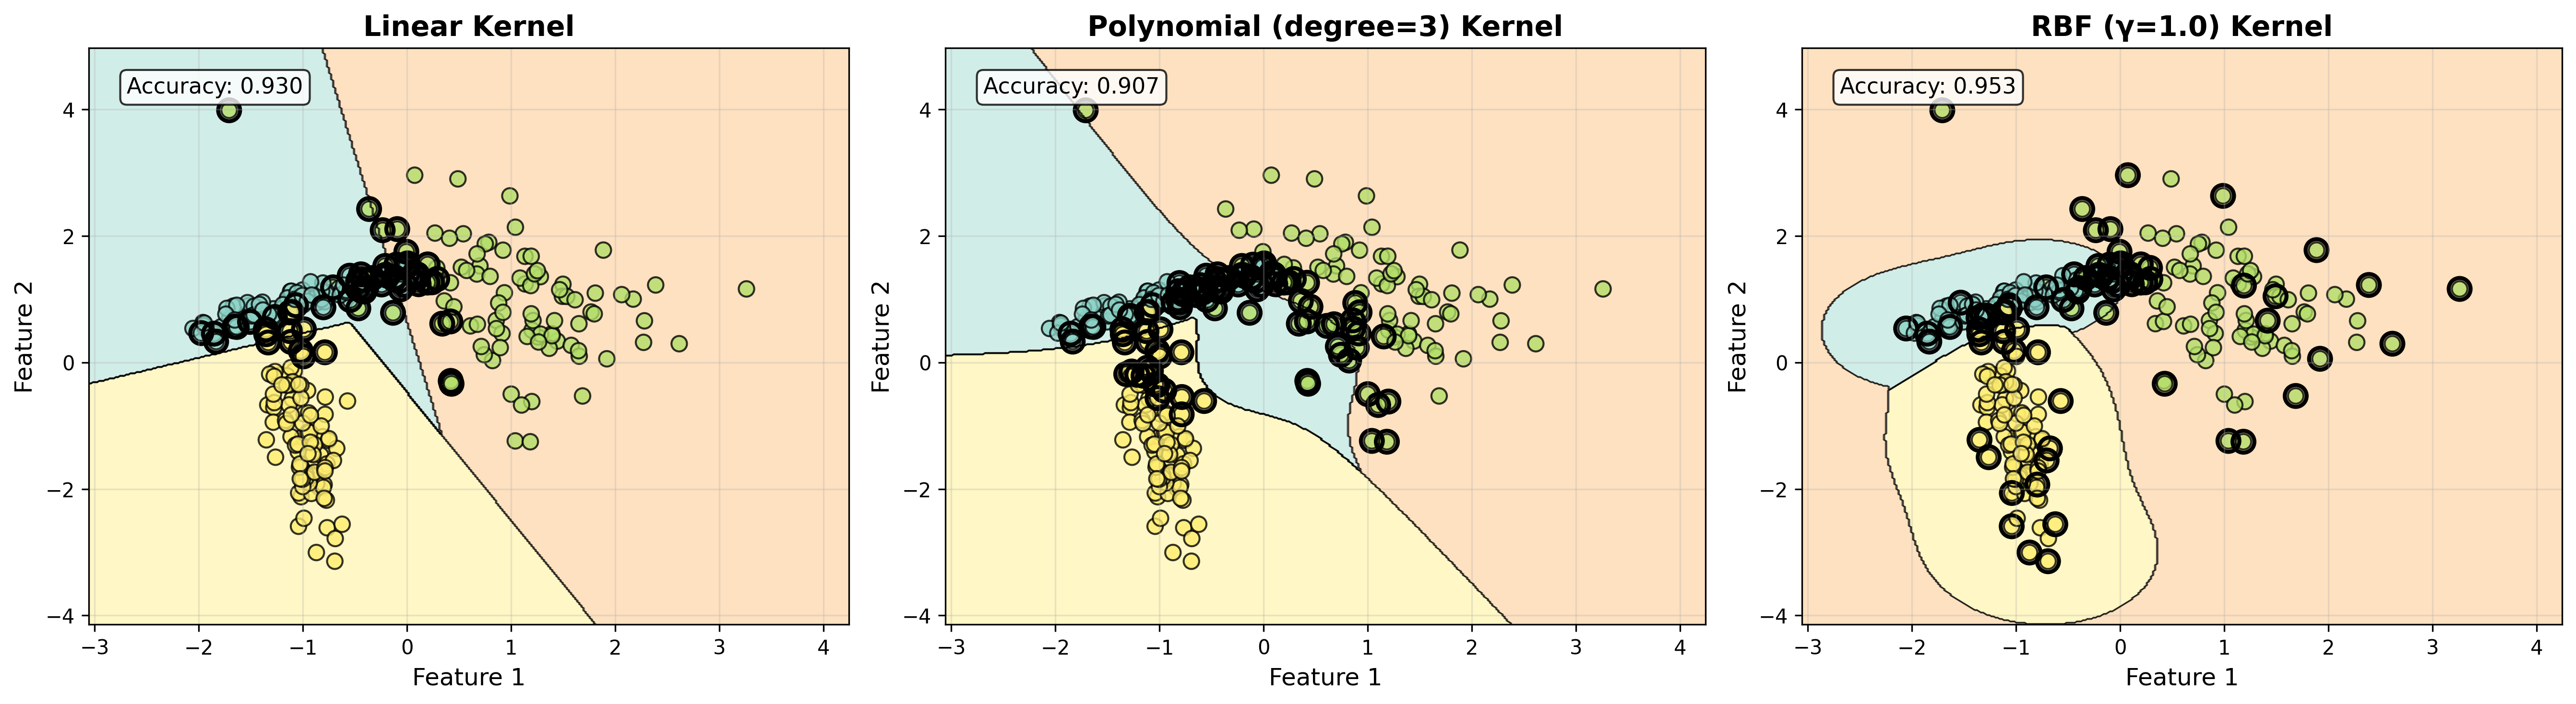
\includegraphics[width=\textwidth]{../figures/kernel_multiclass_comparison.png}
\end{center}

\begin{columns}[t]
\begin{column}{0.48\textwidth}
\textbf{Performance Analysis:}
\vspace{0.2cm}

\begin{itemize}
\setlength{\itemsep}{1pt}
\item \textcolor{blue}{\textbf{Linear Kernel:}} Simple boundaries, good for high-dim data
\item \textcolor{red}{\textbf{Polynomial Kernel:}} Captures feature interactions
\item \textcolor{green}{\textbf{RBF Kernel:}} Most flexible, handles complex patterns
\end{itemize}

\vspace{0.3cm}
\textbf{Selection Criteria:}
\begin{itemize}
\setlength{\itemsep}{1pt}
\item Dataset size and dimensionality
\item Computational resources
\item Interpretability requirements
\item Cross-validation performance
\end{itemize}
\end{column}

\begin{column}{0.48\textwidth}
\textbf{Multi-class Considerations:}
\vspace{0.2cm}

\begin{itemize}
\setlength{\itemsep}{1pt}
\item \textbf{Class balance:} Equal vs imbalanced classes
\item \textbf{Separability:} Linear vs non-linear boundaries
\item \textbf{Noise sensitivity:} Robust vs sensitive kernels
\end{itemize}

\vspace{0.3cm}
\textbf{Hyperparameter Tuning:}
\begin{itemize}
\setlength{\itemsep}{1pt}
\item Grid search over kernel parameters
\item Cross-validation for each class combination
\item Balanced accuracy metrics
\end{itemize}

\vspace{0.3cm}
\begin{alertblock}{Best Practice}
Start with RBF kernel and tune $C$ and $\gamma$ using cross-validation.
\end{alertblock}
\end{column}
\end{columns}
\end{frame}

\section{Kernel Methods for Regression}

\begin{frame}{Support Vector Regression (SVR)}
\begin{columns}[t]
\begin{column}{0.48\textwidth}
\begin{block}{SVR Concept}
Extend SVM to regression by finding a function that deviates from target values by at most $\epsilon$, while being as flat as possible.
\end{block}

\vspace{0.3cm}
\textbf{Linear SVR:}
$$f(x) = w^T x + b$$

\vspace{0.3cm}
\textbf{Optimization Problem:}
\begin{align}
\min_{w,b,\xi,\xi^*} \quad &\frac{1}{2}\|w\|^2 + C\sum_{i=1}^n(\xi_i + \xi_i^*) \\
\text{subject to} \quad &y_i - w^T x_i - b \leq \epsilon + \xi_i \\
&w^T x_i + b - y_i \leq \epsilon + \xi_i^* \\
&\xi_i, \xi_i^* \geq 0
\end{align}

\vspace{0.3cm}
\textbf{$\epsilon$-insensitive Loss:}
$$L_\epsilon(y, f(x)) = \max(0, |y - f(x)| - \epsilon)$$
\end{column}

\begin{column}{0.48\textwidth}
\textbf{Key Parameters:}
\vspace{0.2cm}

\begin{itemize}
\setlength{\itemsep}{1pt}
\item \textbf{$\epsilon$:} Width of insensitive zone
\item \textbf{$C$:} Regularization parameter
\item \textbf{Kernel parameters:} $\gamma$ for RBF, etc.
\end{itemize}

\vspace{0.3cm}
\textbf{Dual Formulation:}
\begin{align}
f(x) = \sum_{i=1}^n (\alpha_i - \alpha_i^*) K(x_i, x) + b
\end{align}

where $\alpha_i, \alpha_i^* \geq 0$ are Lagrange multipliers.

\vspace{0.3cm}
\textbf{Support Vectors:}
\begin{itemize}
\setlength{\itemsep}{1pt}
\item Points outside $\epsilon$-tube
\item $\alpha_i > 0$ or $\alpha_i^* > 0$
\item Determine the regression function
\end{itemize}

\vspace{0.3cm}
\begin{alertblock}{Sparsity}
Many $\alpha_i = \alpha_i^* = 0$, leading to sparse solutions.
\end{alertblock}
\end{column}
\end{columns}
\end{frame}

\begin{frame}{SVR Demonstration}
\begin{center}
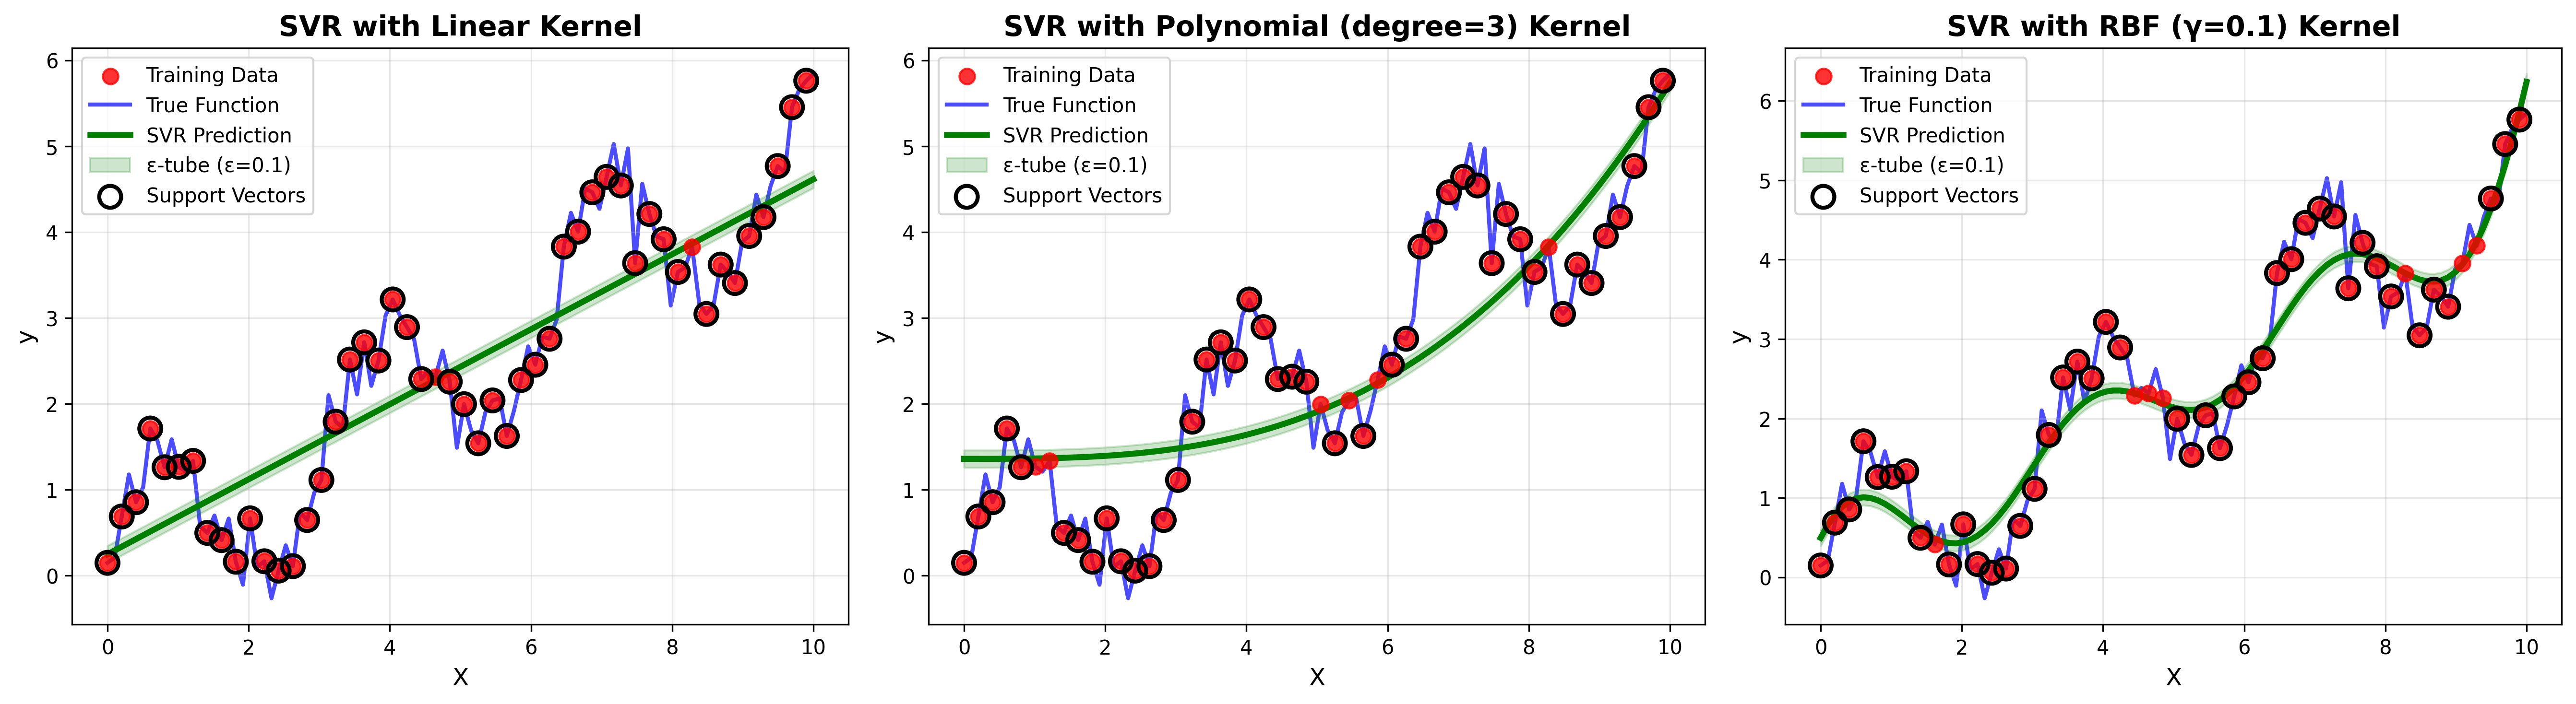
\includegraphics[width=\textwidth]{../figures/svr_demonstration.png}
\end{center}

\begin{columns}[t]
\begin{column}{0.32\textwidth}
\begin{block}{Linear SVR}
\begin{itemize}
\setlength{\itemsep}{1pt}
\item Simple linear relationship
\item Good for linear trends
\item Fast computation
\end{itemize}
\end{block}
\end{column}

\begin{column}{0.32\textwidth}
\begin{block}{Polynomial SVR}
\begin{itemize}
\setlength{\itemsep}{1pt}
\item Captures polynomial trends
\item Risk of overfitting
\item Degree selection important
\end{itemize}
\end{block}
\end{column}

\begin{column}{0.32\textwidth}
\begin{block}{RBF SVR}
\begin{itemize}
\setlength{\itemsep}{1pt}
\item Most flexible
\item Handles non-linear patterns
\item Requires parameter tuning
\end{itemize}
\end{block}
\end{column}
\end{columns}
\end{frame}

\begin{frame}{Effect of $\epsilon$ Parameter in SVR}
\begin{center}
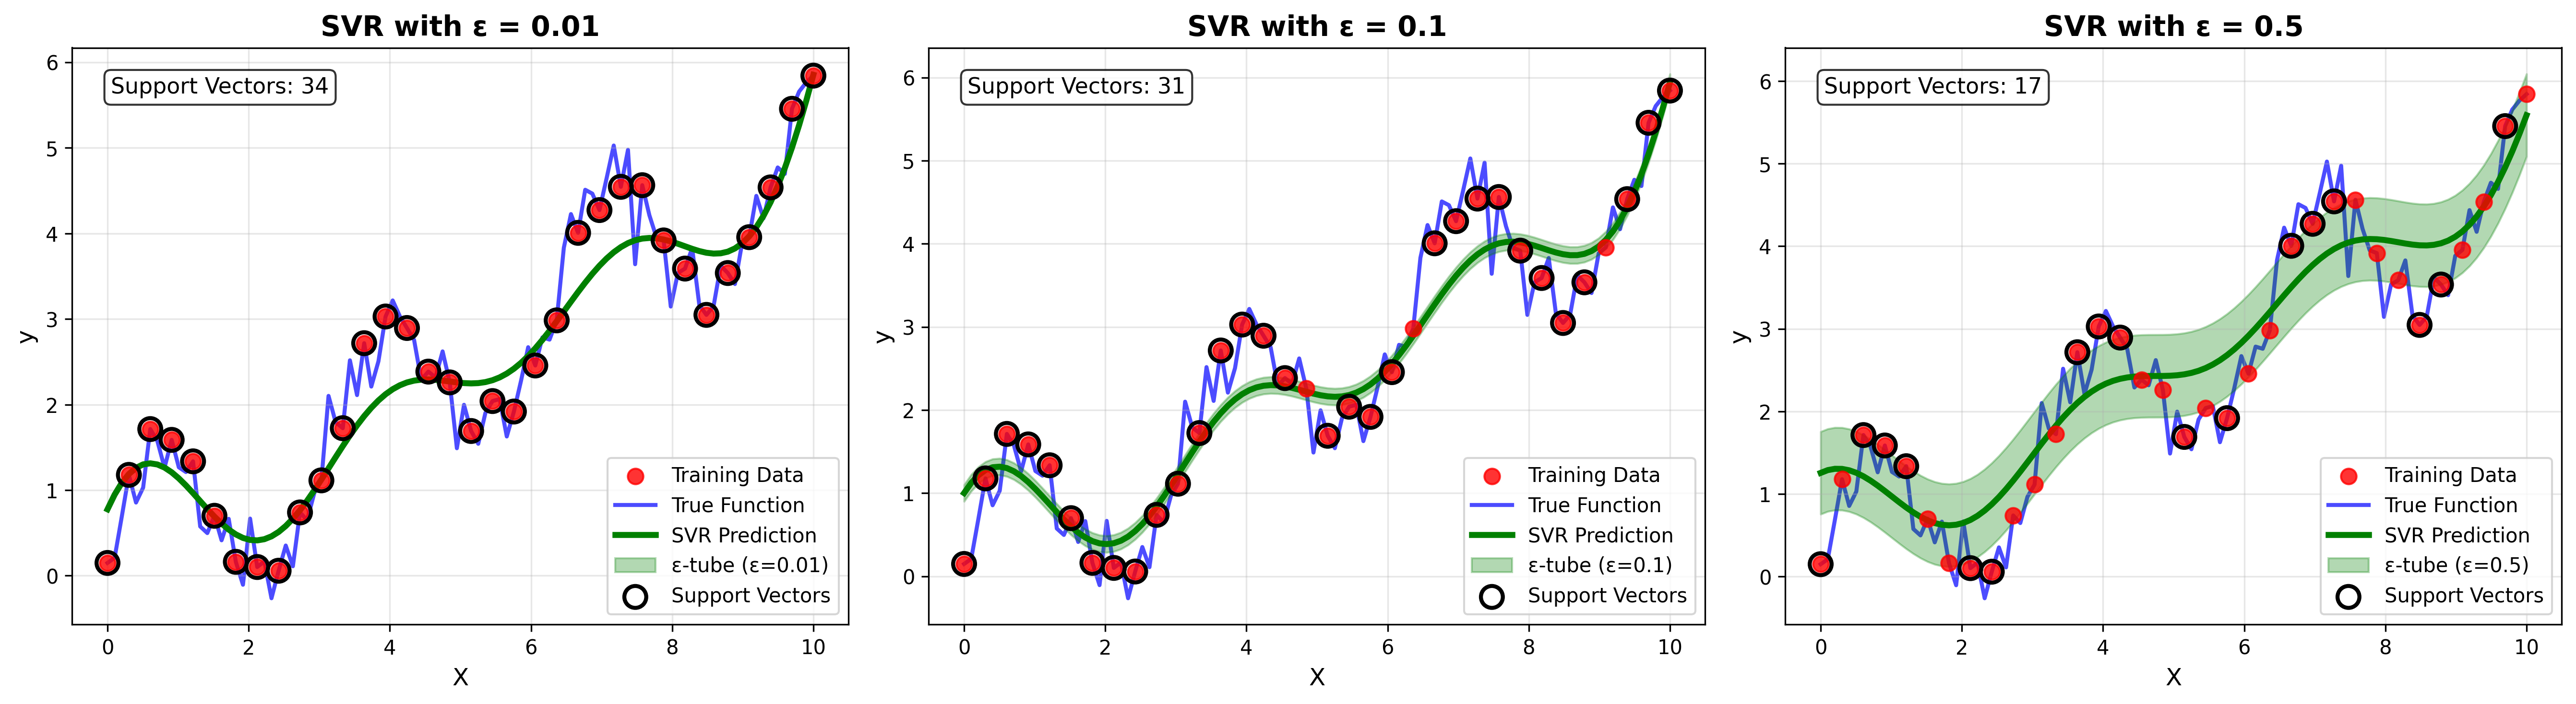
\includegraphics[width=\textwidth]{../figures/epsilon_parameter_effect.png}
\end{center}

\begin{columns}[t]
\begin{column}{0.48\textwidth}
\textbf{$\epsilon$ Parameter Effects:}
\vspace{0.2cm}

\begin{itemize}
\setlength{\itemsep}{1pt}
\item \textbf{Small $\epsilon$ (0.01):} Tight fit, many support vectors
\item \textbf{Medium $\epsilon$ (0.1):} Balanced complexity
\item \textbf{Large $\epsilon$ (0.5):} Loose fit, fewer support vectors
\end{itemize}

\vspace{0.3cm}
\textbf{Trade-offs:}
\begin{itemize}
\setlength{\itemsep}{1pt}
\item \textcolor{red}{\textbf{Small $\epsilon$:}} Low bias, high variance
\item \textcolor{green}{\textbf{Large $\epsilon$:}} High bias, low variance
\item \textcolor{blue}{\textbf{Sparsity:}} Larger $\epsilon$ $\Rightarrow$ fewer support vectors
\end{itemize}
\end{column}

\begin{column}{0.48\textwidth}
\textbf{Selection Guidelines:}
\vspace{0.2cm}

\begin{itemize}
\setlength{\itemsep}{1pt}
\item Cross-validation for optimal $\epsilon$
\item Consider noise level in data
\item Balance accuracy vs complexity
\end{itemize}

\vspace{0.3cm}
\textbf{Practical Values:}
\begin{itemize}
\setlength{\itemsep}{1pt}
\item Start with $\epsilon = 0.1$
\item Scale with target variable range
\item Grid search with $C$ and kernel parameters
\end{itemize}

\vspace{0.3cm}
\begin{alertblock}{Rule of Thumb}
Set $\epsilon \approx \frac{\text{std}(y)}{10}$ as starting point.
\end{alertblock}
\end{column}
\end{columns}
\end{frame}

\section{Support Vector Regression}

\begin{frame}{Kernel Ridge Regression vs SVR}
\begin{center}
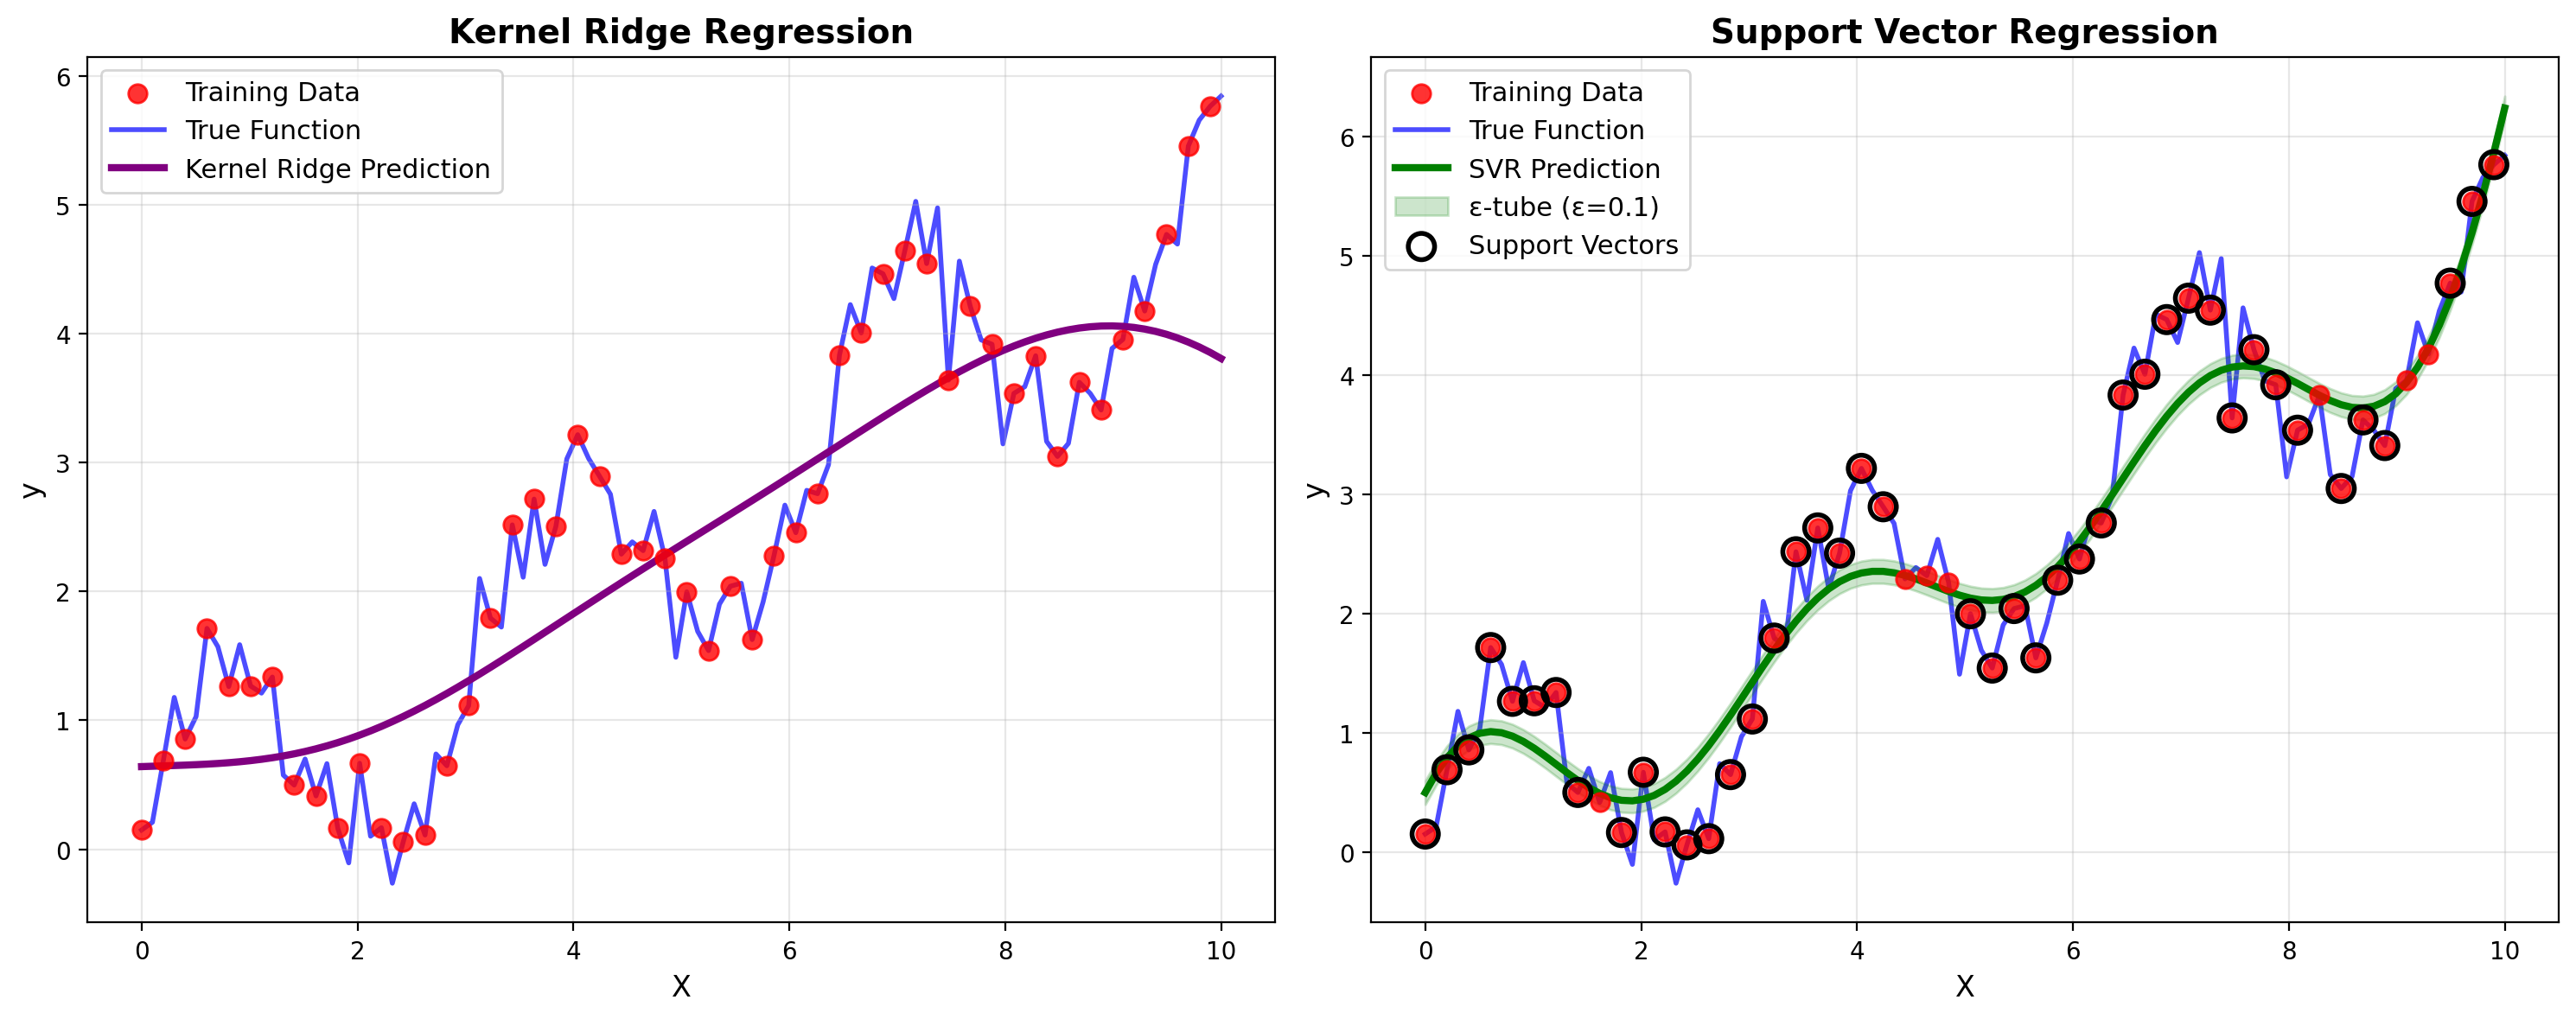
\includegraphics[width=\textwidth]{../figures/kernel_ridge_vs_svr.png}
\end{center}

\begin{columns}[t]
\begin{column}{0.48\textwidth}
\begin{block}{Kernel Ridge Regression}
\textbf{Objective:}
$$\min_\alpha \|\mathbf{K}\alpha - y\|^2 + \lambda \alpha^T \mathbf{K} \alpha$$

\textbf{Solution:}
$$\alpha = (\mathbf{K} + \lambda \mathbf{I})^{-1} y$$

\textbf{Prediction:}
$$f(x) = \sum_{i=1}^n \alpha_i K(x_i, x)$$
\end{block}

\vspace{0.3cm}
\textbf{Properties:}
\begin{itemize}
\setlength{\itemsep}{1pt}
\item Non-sparse solution
\item Closed-form solution
\item Fast training for small datasets
\end{itemize}
\end{column}

\begin{column}{0.48\textwidth}
\begin{block}{Support Vector Regression}
\textbf{Objective:}
$$\min_{w,b,\xi} \frac{1}{2}\|w\|^2 + C\sum_i (\xi_i + \xi_i^*)$$

\textbf{Constraints:}
$$|y_i - f(x_i)| \leq \epsilon + \xi_i$$

\textbf{Prediction:}
$$f(x) = \sum_{\text{SV}} (\alpha_i - \alpha_i^*) K(x_i, x) + b$$
\end{block}

\vspace{0.3cm}
\textbf{Properties:}
\begin{itemize}
\setlength{\itemsep}{1pt}
\item Sparse solution (support vectors)
\item Robust to outliers ($\epsilon$-insensitive)
\item Requires quadratic programming
\end{itemize}
\end{column}
\end{columns}
\end{frame}

\section{Kernel Ridge Regression}

\begin{frame}{Regularization in Kernel Regression}
\begin{center}
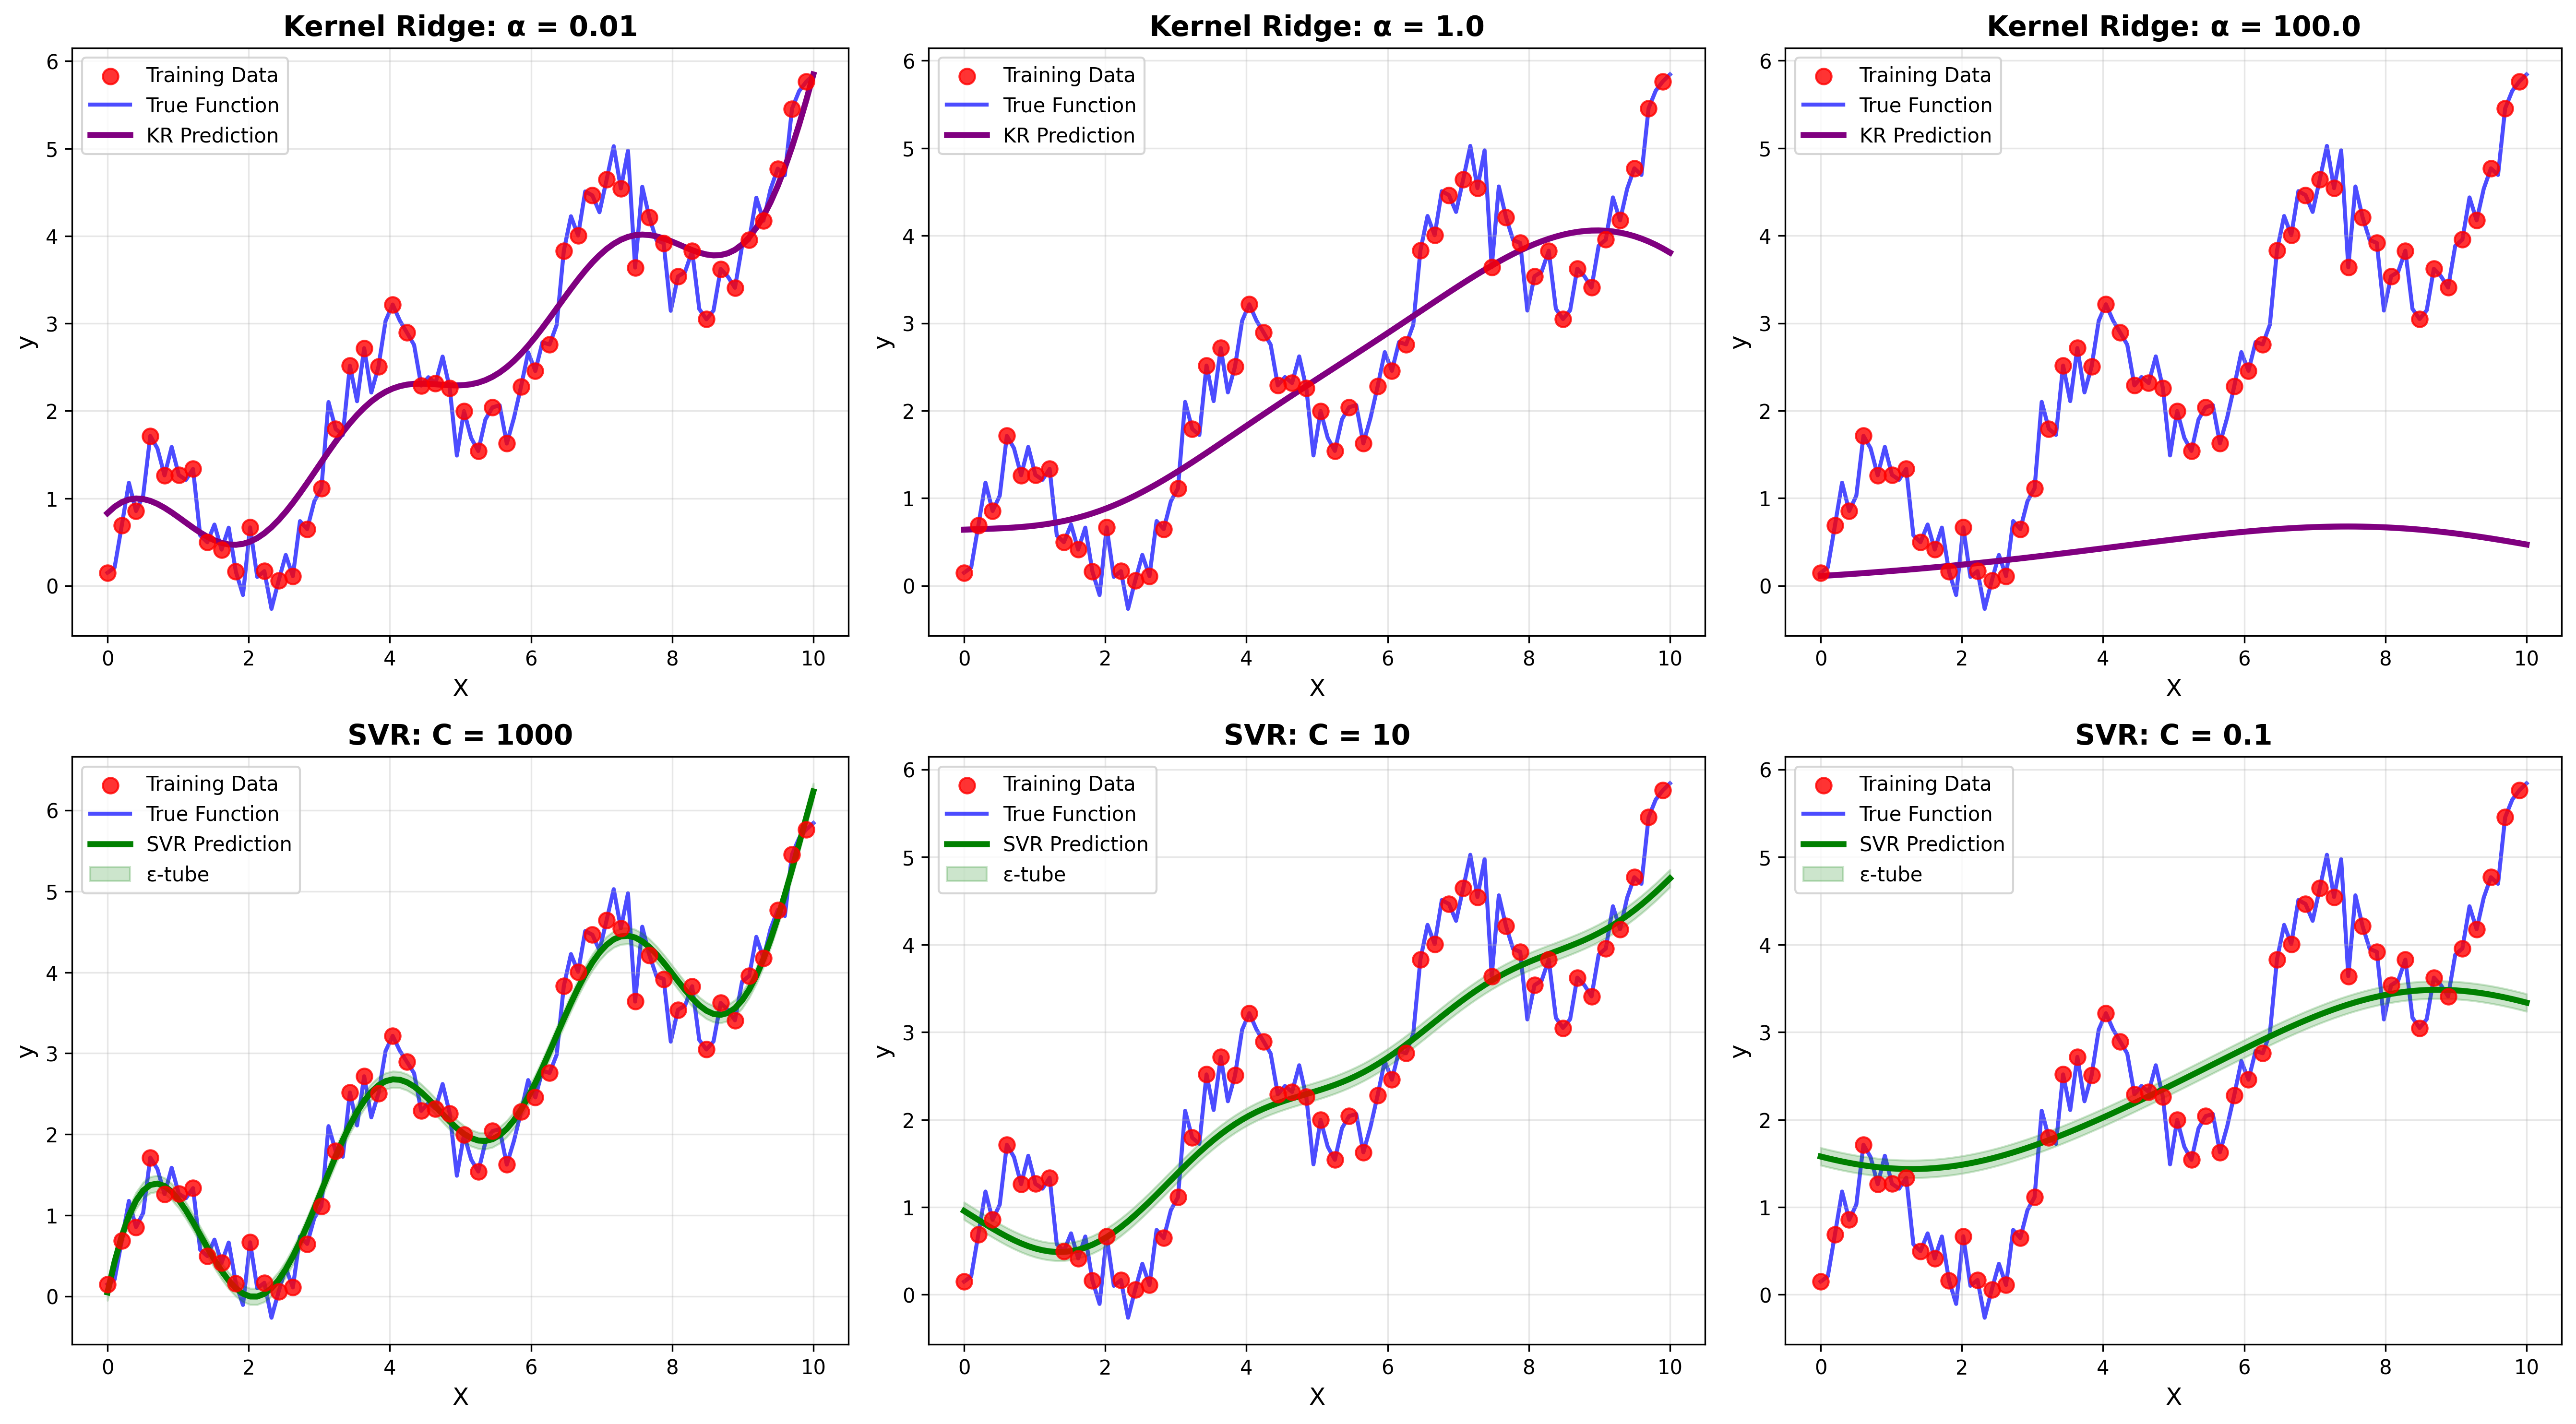
\includegraphics[width=\textwidth]{../figures/regularization_comparison.png}
\end{center}

\begin{columns}[t]
\begin{column}{0.48\textwidth}
\textbf{Kernel Ridge Regularization ($\alpha$):}
\vspace{0.2cm}

\begin{itemize}
\setlength{\itemsep}{1pt}
\item \textbf{Small $\alpha$ (0.01):} Low regularization, overfitting risk
\item \textbf{Medium $\alpha$ (1.0):} Balanced regularization
\item \textbf{Large $\alpha$ (100):} High regularization, underfitting risk
\end{itemize}

\vspace{0.3cm}
\textbf{Regularization Effect:}
$$\min_f \sum_{i=1}^n (y_i - f(x_i))^2 + \alpha \|f\|_{\mathcal{H}}^2$$

Controls smoothness of function $f$ in reproducing kernel Hilbert space $\mathcal{H}$.
\end{column}

\begin{column}{0.48\textwidth}
\textbf{SVR Regularization ($C$):}
\vspace{0.2cm}

\begin{itemize}
\setlength{\itemsep}{1pt}
\item \textbf{High $C$ (1000):} Low regularization, complex model
\item \textbf{Medium $C$ (10):} Balanced complexity
\item \textbf{Low $C$ (0.1):} High regularization, simple model
\end{itemize}

\vspace{0.3cm}
\textbf{Parameter Relationships:}
\begin{align}
\text{Kernel Ridge: } &\alpha \text{ large} \Rightarrow \text{more regularization} \\
\text{SVR: } &C \text{ large} \Rightarrow \text{less regularization}
\end{align}

\vspace{0.2cm}
Approximately: $C \approx \frac{1}{\alpha}$
\end{column}
\end{columns}
\end{frame}

\begin{frame}{Worked Example: RBF Kernel Computation}
\begin{columns}[t]
\begin{column}{0.48\textwidth}
\textbf{Problem Setup:}
\vspace{0.2cm}

Given two points:
\begin{align}
x_1 &= (1, 2) \\
x_2 &= (3, 1)
\end{align}

Compute RBF kernel with $\gamma = 0.5$:
$$K(x_1, x_2) = \exp(-\gamma \|x_1 - x_2\|^2)$$

\vspace{0.3cm}
\textbf{Step 1: Compute distance}
\begin{align}
x_1 - x_2 &= (1, 2) - (3, 1) = (-2, 1) \\
\|x_1 - x_2\|^2 &= (-2)^2 + 1^2 = 4 + 1 = 5
\end{align}

\vspace{0.3cm}
\textbf{Step 2: Apply kernel}
\begin{align}
K(x_1, x_2) &= \exp(-0.5 \times 5) \\
&= \exp(-2.5) \\
&\approx 0.082
\end{align}
\end{column}

\begin{column}{0.48\textwidth}
\textbf{Interpretation:}
\vspace{0.2cm}

\begin{itemize}
\setlength{\itemsep}{1pt}
\item Points are moderately far apart
\item Kernel value is small (0.082)
\item Indicates low similarity
\end{itemize}

\vspace{0.3cm}
\textbf{Compare with closer points:}
\vspace{0.2cm}

For $x_1 = (1, 2)$ and $x_3 = (1.1, 2.1)$:
\begin{align}
\|x_1 - x_3\|^2 &= (0.1)^2 + (0.1)^2 = 0.02 \\
K(x_1, x_3) &= \exp(-0.5 \times 0.02) = \exp(-0.01) \\
&\approx 0.99
\end{align}

\vspace{0.3cm}
\textbf{Effect of $\gamma$:}
\begin{itemize}
\setlength{\itemsep}{1pt}
\item Large $\gamma$: Rapid decay, local influence
\item Small $\gamma$: Slow decay, global influence
\end{itemize}

\vspace{0.3cm}
\begin{alertblock}{Key Insight}
RBF kernel measures similarity through Euclidean distance in input space.
\end{alertblock}
\end{column}
\end{columns}
\end{frame}

\begin{frame}{Practical Implementation Tips}
\begin{columns}[t]
\begin{column}{0.48\textwidth}
\textbf{Data Preprocessing:}
\vspace{0.2cm}

\begin{itemize}
\setlength{\itemsep}{1pt}
\item \textcolor{blue}{\textbf{Feature Scaling:}} Critical for RBF kernels
\item \textcolor{red}{\textbf{Normalization:}} StandardScaler or MinMaxScaler
\item \textcolor{green}{\textbf{Missing Values:}} Handle before kernel computation
\end{itemize}

\vspace{0.3cm}
\textbf{Hyperparameter Tuning:}
\vspace{0.2cm}

\begin{block}{Grid Search Example}
\scriptsize
\texttt{param\_grid = \{} \\
\texttt{    'C': [0.1, 1, 10, 100],} \\
\texttt{    'gamma': [0.001, 0.01, 0.1, 1],} \\
\texttt{    'kernel': ['rbf', 'poly', 'linear']} \\
\texttt{\}}
\end{block}

\vspace{0.3cm}
\textbf{Performance Considerations:}
\begin{itemize}
\setlength{\itemsep}{1pt}
\item Linear kernel: $\mathcal{O}(n \times d)$
\item RBF kernel: $\mathcal{O}(n \times d)$ per evaluation
\item Training complexity: $\mathcal{O}(n^2)$ to $\mathcal{O}(n^3)$
\end{itemize}
\end{column}

\begin{column}{0.48\textwidth}
\textbf{Model Selection:}
\vspace{0.2cm}

\begin{enumerate}
\setlength{\itemsep}{1pt}
\item Start with RBF kernel
\item Use cross-validation
\item Compare with linear kernel
\item Consider computational constraints
\end{enumerate}

\vspace{0.3cm}
\textbf{Common Pitfalls:}
\vspace{0.2cm}

\begin{alertblock}{Avoid These}
\begin{itemize}
\setlength{\itemsep}{1pt}
\item Forgetting to scale features
\item Using default parameters
\item Ignoring class imbalance
\item Overfitting with complex kernels
\end{itemize}
\end{alertblock}

\vspace{0.3cm}
\textbf{Debugging Tips:}
\begin{itemize}
\setlength{\itemsep}{1pt}
\item Check kernel matrix properties
\item Visualize decision boundaries
\item Monitor support vector counts
\item Validate on holdout set
\end{itemize}

\vspace{0.3cm}
\textbf{Software Libraries:}
\begin{itemize}
\setlength{\itemsep}{1pt}
\item \texttt{scikit-learn}: General purpose
\item \texttt{libsvm}: High performance
\item \texttt{thundersvm}: GPU acceleration
\end{itemize}
\end{column}
\end{columns}
\end{frame}

\section{Parametric vs Non-parametric Models}

\begin{frame}{Understanding Model Types}
\begin{columns}[t]
\begin{column}{0.48\textwidth}
\textbf{Parametric Models:}
\vspace{0.2cm}

\begin{block}{Definition}
Fixed number of parameters independent of training set size. Make strong assumptions about functional form.
\end{block}

\vspace{0.3cm}
\textbf{Examples:}
\begin{itemize}
\setlength{\itemsep}{1pt}
\item \textbf{Linear Regression:} $f(x) = w^T x + b$
\item \textbf{Logistic Regression:} $p = \sigma(w^T x + b)$
\item \textbf{Perceptron:} Fixed decision boundary
\item \textbf{Neural Networks:} Fixed architecture
\end{itemize}

\vspace{0.3cm}
\textbf{Characteristics:}
\begin{itemize}
\setlength{\itemsep}{1pt}
\item Fast training and prediction
\item Strong inductive bias
\item May underfit complex data
\item Interpretable parameters
\end{itemize}
\end{column}

\begin{column}{0.48\textwidth}
\textbf{Non-parametric Models:}
\vspace{0.2cm}

\begin{block}{Definition}
Number of parameters grows with training data size. Make minimal assumptions about functional form.
\end{block}

\vspace{0.3cm}
\textbf{Examples:}
\begin{itemize}
\setlength{\itemsep}{1pt}
\item \textbf{k-NN:} Stores all training data
\item \textbf{Decision Trees:} Adaptive structure
\item \textbf{Kernel Methods:} Support vector representation
\item \textbf{Gaussian Processes:} Infinite parameters
\end{itemize}

\vspace{0.3cm}
\textbf{Characteristics:}
\begin{itemize}
\setlength{\itemsep}{1pt}
\item Flexible representation
\item Can fit complex patterns
\item Risk of overfitting
\item Higher computational cost
\end{itemize}
\end{column}
\end{columns}
\end{frame}

\begin{frame}{Kernel Methods: The Non-parametric Perspective}
\begin{columns}[t]
\begin{column}{0.48\textwidth}
\textbf{Why SVMs are Non-parametric:}
\vspace{0.3cm}

\begin{alertblock}{Key Insight}
SVM decision function depends on support vectors, whose number grows with data complexity, not fixed in advance.
\end{alertblock}

\vspace{0.3cm}
\textbf{Decision Function:}
$$f(x) = \sum_{i \in SV} \alpha_i y_i K(x_i, x) + b$$

\vspace{0.2cm}
\begin{itemize}
\setlength{\itemsep}{1pt}
\item Number of support vectors $|SV|$ varies
\item Complex data $\Rightarrow$ more support vectors
\item Simple data $\Rightarrow$ fewer support vectors
\end{itemize}

\vspace{0.3cm}
\textbf{Adaptive Complexity:}
\begin{itemize}
\setlength{\itemsep}{1pt}
\item Model complexity adapts to data
\item Automatic feature selection
\item Sparse representation via support vectors
\end{itemize}
\end{column}

\begin{column}{0.48\textwidth}
\textbf{Comparison with Other Methods:}
\vspace{0.3cm}

\begin{block}{Parametric Linear Classifier}
$$f(x) = w^T x + b$$
Fixed $d+1$ parameters regardless of training set size.
\end{block}

\vspace{0.3cm}
\begin{block}{Non-parametric SVM}
$$f(x) = \sum_{i=1}^{n_{sv}} \alpha_i y_i K(x_i, x) + b$$
$n_{sv}$ support vectors determined by data.
\end{block}

\vspace{0.3cm}
\textbf{Benefits of Non-parametric Approach:}
\begin{itemize}
\setlength{\itemsep}{1pt}
\item \textcolor{blue}{\textbf{Flexibility:}} No assumptions about decision boundary shape
\item \textcolor{red}{\textbf{Universality:}} Can approximate any function (with appropriate kernel)
\item \textcolor{green}{\textbf{Robustness:}} Less sensitive to model specification
\end{itemize}
\end{column}
\end{columns}
\end{frame}

\begin{frame}{Kernel Functions and Function Spaces}
\begin{columns}[t]
\begin{column}{0.48\textwidth}
\textbf{Reproducing Kernel Hilbert Space (RKHS):}
\vspace{0.3cm}

\begin{block}{Mathematical Framework}
Kernel $K$ defines an infinite-dimensional feature space $\mathcal{H}$ where linear methods become non-linear in original space.
\end{block}

\vspace{0.3cm}
\textbf{Key Properties:}
\begin{align}
\phi: \mathcal{X} &\to \mathcal{H} \\
K(x, x') &= \langle \phi(x), \phi(x') \rangle_{\mathcal{H}}
\end{align}

\vspace{0.3cm}
\textbf{Universal Approximation:}
\begin{itemize}
\setlength{\itemsep}{1pt}
\item RBF kernels are universal approximators
\item Can represent any continuous function
\item Given sufficient training data
\end{itemize}

\vspace{0.3cm}
\begin{alertblock}{Non-parametric Power}
Kernel methods can learn arbitrarily complex decision boundaries without specifying the form in advance.
\end{alertblock}
\end{column}

\begin{column}{0.48\textwidth}
\textbf{Practical Implications:}
\vspace{0.3cm}

\textbf{Model Selection Strategy:}
\begin{itemize}
\setlength{\itemsep}{1pt}
\item \textbf{Start Simple:} Linear kernel first
\item \textbf{Add Complexity:} Polynomial → RBF
\item \textbf{Cross-validate:} Choose optimal kernel and parameters
\end{itemize}

\vspace{0.3cm}
\textbf{Trade-offs:}

\begin{block}{Parametric Advantage}
\begin{itemize}
\setlength{\itemsep}{1pt}
\item Fast training and prediction
\item Lower memory requirements
\item Better interpretability
\end{itemize}
\end{block}

\begin{block}{Non-parametric Advantage}
\begin{itemize}
\setlength{\itemsep}{1pt}
\item Higher representational power
\item Better fit to complex data
\item Fewer modeling assumptions
\end{itemize}
\end{block}

\vspace{0.3cm}
\textbf{When to Use Kernel Methods:}
\begin{itemize}
\setlength{\itemsep}{1pt}
\item Non-linear relationships in data
\item High-dimensional feature spaces
\item Need for flexible decision boundaries
\end{itemize}
\end{column}
\end{columns}
\end{frame}

\begin{frame}{Summary and Key Takeaways}
\begin{columns}[t]
\begin{column}{0.48\textwidth}
\textbf{Core Concepts Learned:}
\vspace{0.2cm}

\begin{itemize}
\setlength{\itemsep}{1pt}
\item \textcolor{blue}{\textbf{Kernel Trick:}} Implicit high-dimensional mapping
\item \textcolor{red}{\textbf{Support Vectors:}} Sparse representation
\item \textcolor{green}{\textbf{Margin Maximization:}} Generalization principle
\item \textcolor{purple}{\textbf{Non-linear Separation:}} Via kernels
\end{itemize}

\vspace{0.3cm}
\textbf{Main Algorithms:}
\begin{itemize}
\setlength{\itemsep}{1pt}
\item \textbf{SVM:} Classification with maximum margin
\item \textbf{SVR:} Regression with $\epsilon$-insensitive loss
\item \textbf{Kernel Ridge:} Regularized regression
\item \textbf{Multi-class:} Extensions to multiple classes
\end{itemize}

\vspace{0.3cm}
\textbf{Key Kernels:}
\begin{itemize}
\setlength{\itemsep}{1pt}
\item Linear, Polynomial, RBF, Sigmoid
\item Mercer's theorem for validity
\item Multiple kernel learning
\end{itemize}
\end{column}

\begin{column}{0.48\textwidth}
\textbf{Practical Guidelines:}
\vspace{0.2cm}

\begin{block}{When to Use Kernel Methods}
\begin{itemize}
\setlength{\itemsep}{1pt}
\item Non-linear relationships in data
\item Need for sparse solutions
\item Strong theoretical guarantees required
\item Medium-sized datasets
\end{itemize}
\end{block}

\vspace{0.3cm}
\textbf{Parameter Selection:}
\begin{itemize}
\setlength{\itemsep}{1pt}
\item \textbf{C:} Start with 1.0, tune via CV
\item \textbf{$\gamma$:} Start with $\frac{1}{\text{n\_features}}$
\item \textbf{$\epsilon$:} Start with 0.1 for SVR
\end{itemize}

\vspace{0.3cm}
\textbf{Limitations:}
\begin{itemize}
\setlength{\itemsep}{1pt}
\item Computational complexity: $\mathcal{O}(n^2)$ to $\mathcal{O}(n^3)$
\item Memory requirements: Store kernel matrix
\item Parameter sensitivity
\item Not suitable for very large datasets
\end{itemize}

\vspace{0.3cm}
\begin{alertblock}{Next Steps}
Explore deep learning for automatic feature learning in high-dimensional spaces.
\end{alertblock}
\end{column}
\end{columns}
\end{frame}

\end{document}